\chapter{Di-$b$-jet Search: Search Phase}
\label{sec:bkg}

The role of the search phase is to identify
if there is any evidence of a resonance
in the~\mjj~spectra of the di-$b$-jet events selected.
This is carred out in two parts;
firstly a background fit is used to estimate
the~\mjj~distribution of the QCD dijet background.
Then, the difference between the data
and the background estimation is used 
to search 
for a significant excess that would be evidence
of a resonance.

In this chapter
I will describe
the details of the $m_{jj}$ spectra used in the analysis
(Section~\ref{sec:bkg-mjj}),
the background estimation strategy
(Section~\ref{sec:bkg-fit})
the technique used to search for excesses
(Section~\ref{sec:bkg-bh})
and then I will present the search phase
validation and results from each of the data sets.

\section{Invariant Dijet Mass Spectrum}
\label{sec:bkg-mjj}

The invariant mass spectrum is the number of events
with an invariant mass~\mjj~
of the leading and subleading jet.
The~\mjj~spectrum is analysed in a binned histogram,
the bin size is chosen to give a smooth spectrum
and to be larger than the mass resolution of the detector \textbf{LM Fix: I though mass res was ~5\%. Check}.
The exact bins are chosen following the study found here~\cite{dijet-mori16_int}
and are shown in Appendix~\ref{app:dijet_bins}.

There is a different~\mjj~spectrum for each
$b$-tagging category considered,
and an independant search phase will be performed for both.

%Which is defined as;
%begin{equation}
% \mjj = \sqrt{ p^\mu_{L}^2 + p^\mu_{SL}^2 }
%end{equation}
%here $p^\mu_{L}$ and $p^\mu_{SL}^2$ are the four vectors of the leading and su


\section{Background Estimation}
\label{sec:bkg-fit}

Many analyses at ATLAS use Monte-Carlo simulation
to model backgrounds~\cite{obj-Hbb}.
However, simulation is not used to model the
background in the di-$b$-jet search due to three problems;
firstly it is difficult to produce Monte-Carlo simulation at high-enough statistical precision,
secondly there are large theoretical uncertainties for Monte-Carlo QCD
(such as PDF uncertainties and choice of renormalisation scale)
and finally there are large experimental uncertainties affecting
data-simulation comparisons (such as jet energy scale).

Instead, the background is described using a smooth fit function.
This approach utilises the fact that the QCD dijet spectrum
is smoothly falling with respect to~\mjj,
as discussed in Section~\ref{sec:theo-qcd-dijet_features}.
Fit functions have been widely used
in a wide range of searches for resonances on smoothly falling backgrounds
including previous dijet and di-$b$-jet searches~\cite{dijet-mori16_paper,dibjet-mori16_paper}.

This approach gives two requirements on a fit function;
firstly the fit function must be able to describe the di-$b$-jet spectrum from QCD,
including any detector or reconstruction effects that could impact the shape such as $b$-tagging.
Secondly,  the fit function used must be contrained enough
such that there is no bias if there is a resonance present in the di-$b$-jet spectrum.
As evidence of such a resonance is found when the data diverges from the fit,
such a bias could reduce the sensitivity to signal.
The fit functions considered in this analysis will be described in the following section.

For any given fit function, 
data is used to determine the parameters of the fit function.
This is done by minimising the negative log likelihood,
where the likelihood is calculated from comparing
the binned data to the fit function
under the assumption of poisson-like errors.

\subsection{Dijet Fit Functions}
\label{sec:bkg-bkg_func}

%\begin{equation}
%  f(x)=p_1(1-x)^{p_2}(x)^{p_3+p_4\ln{x}+p_5(\ln{x})^{2}}
%  %p_6(\ln{x})^{3}%},
%\label{eqn:bkg-fit}
%\end{equation}
%where $p_i$ are fit parameters, and $x=m_{jj}/\sqrt{s}$.

%Degrees of freedom can be removed to give a family of dijet fit functions which have a number of parameters ranging from 3 to 6.
%The 3 parameter dijet fit function is defined by setting $p_{i} = 0$ for $i > 3$ in Table~\ref{tab:bkg-fit}
%and the definition is equivalent for the 4 and 5 parameter dijet fit function.
%There is in addition a 6 parameter dijet fit function where $x=m_{jj}/p_6$.

The di-$b$-jet mass spectrum will be described by the dijet fit functions,
which are a family of functions with a varying number of parameters.
The dijet fit functions are listed in Table~\ref{tab:bkg-fit}.


{\renewcommand{\arraystretch}{1.2}
\begin{table}[!thb]
\centering
\begin{tabular}{|c||c|c|}
  \hline
  Function Name & Equation                                          & $x$ \\
  \hline
  3 parameter   & $f(x)=p_1(1-x)^{p_2}x^{p_3}$                         & $m_{jj}/\sqrt{s}$ \\
  4 parameter   & $f(x)=p_1(1-x)^{p_2}x^{p_3+p_4\ln{x}}$                &$m_{jj}/\sqrt{s}$\\
  5 parameter   & $f(x)=p_1(1-x)^{p_2}x^{p_3+p_4\ln{x}+p_5(\ln{x})^{2}}$   & $m_{jj}/\sqrt{s}$\\ 
  6 parameter   & $f(x)=p_1(1-x)^{p_2}x^{p_3+p_4\ln{x}+p_5(\ln{x})^{2}}$   &  $m_{jj}/p_6$\\ 
  \hline
\end{tabular}
\caption{The dijet fit function equations. The fit functions are named by the number of free parameters used. $p_{i}$ are the free parameters of the fit function}
\label{tab:bkg-fit}
\end{table}}

The dijet fit functions are motivated using a theoretical understanding of the QCD dijet production
and experience from previous dijet searches~\cite{theo-dijet_harris}.
The 3 parameter dijet fit function has been used in dijet searches beginning with CDF~\cite{dijet-CDF_3par}
and the three components are motivated as follows:
the $p_1$ term gives the normalisation,
the $(1-x)^{p_2}$ term is a common parameterisation for the behaviour of the PDFs with the property of vanishing as $x$ approaches unity,
and the $x^{p_3}$ term is motivated by the $1/m_{kl}$ term in the matrix element (shown in Equation~\ref{eq:theo-qcd_dijet_xs}).
Additional parameters of $x^{p_4\ln{x}}$ and $x^{p_5\ln{x}^{2}}$ have been considered in dijet searches to give an adequete discription of the tail
when large mass ranges are considered~\cite{dijet-CDF_4par,dijet-mori16_int}.
Finally, the $x=m_{jj}/p_6$ term is added as an additional degree of freedom.
This function has been found to provide a satisfactory fit to the leading and next-to-leading-order QCD Monte-Carlo simulation.


Adding additional parameters to the 3 parameter dijet fit function may be required to describe the di-$b$-jet mass spectrum;
especially in large data-sets where small statistical errors reveal finer details of the QCD background shape
and large mass ranges where larger constraints are applied to the fit in each mass range.
However, additional parameters also allow for more flexibility in the background shape
which might cause a fit bias if a resonance is present.
Hence, there is an overall strategy to use the fewest number of parameters
that can adequetely describe the background,
such that sensitivity to signal is maximised.

\subsection{Wilks' Statistic}
\label{sec:bkg-bkg_wilks}

To decide whether a fit function has adequete number of parameters the Wilks' test statistic is used,
as done in previous iterations of both the inclusive and $b$-tagged dijet search~\cite{dijet-mori16_paper,dibjet-mori16_paper}.
The Wilks' test statistic tests the null hypothesis that the nominal fit function contains enough parameters to describe the data
by comparing the nominal to an alternate fit that has 1 extra parameter.
One can calculate the Wilks' test statistic, which is defined as $-\log{(\Lambda)}$, where $\Lambda$ is the likelihood ratio of the nominal and alternate function.
Using Wilks' theorem it is known that for nested functions
\footnote{Nested functions occur when the simpler function can be taken from a more complex function by setting one parameter to a specific value.
  For example the 3 parameter function can be taken from the 4 parameter function when $p_4$ = 0 and so on},
such as the functions in Table~\ref{tab:bkg-fit},
the Wilks' test statistic will follow a $\chi^2$ distribution with 1 degree of freedom~\cite{dibjet-wilks}.
Using this a $p$-value can be calculated for our null hypotheses that the nominal function has sufficient number of parameters.
Such a $p$-value will be referred to as the Wilks' $p$-value throughout this section.

%\subsection{Parameter Optimsation}
%\label{sec:bkg-bkg_param}

\section{BumpHunter Algorithm}
\label{sec:bkg-bh}

Once the background has been modelled using a fit, the next step is to determine
if there is evidence of a resonance in our di-$b$-jet invariant mass spectrum.
As shown in Figure~\ref{fig:evt-dijet_schem} such a resonance would appear as a bump on the smoothly falling background distribution.
This can be observed as a discrepant excess in the~\mjj~spectrum;
where an excess is defined as any set of consecutive bins that contain
more events in data than the background prediction,
and discrepant describes how inconsistent an excess is with the background estimation.
To set this up in terms of hypothesis testing, the null hypothesis, $H_0$,
states that there is only QCD dijet events described by our background function,
whilst the alternate hypothesis, $H_1$, proposes that there is also a resonance at some
unknown mass point in the di-$b$-jet spectrum causing a discrepant excess.

Due to statistical fluctuations in the background,
it is expected that excesses will occur in data even if there is no new physics occuring.
Therefore, to claim evidence of a new resonance a significant excess is required,
which is an excess that is highly unlikely to have occured from such a fluctuation.
To quantify how significant any excess is a $p$-value is used,
where a $p$-value is defined as the probablity of finding an excess which is at least as discrepant as the excess found in data
under the assumption of $H_0$.
Hence, a small $p$-value indicates the excess is inconsistent with the null hypothesis and that new physics is present;
in particle physics it is conventional to consider that a $p$-value below 0.0027 (3 \sigma) is considered as evidence of new physics
whilst a $p$-value below 1 in $\sim$3.5 million (5 \sigma) is considered as the discovery of new physics.

In this analysis the {\sc BumpHunter} algorithm~\cite{dibjet-bh} is employed;
this algorithm uses a test-statistic to 
search for the most discrepant excess in our data-set
and calculate the $p$-value of such an excess.
The BumpHunter test statistic gives a quantitive measure of how discrepant any given excess in data is
under the assumption of $H_0$.
To derive the test statistic let's consider $N$ consecutive bins for which
a total of $d$ data events are found and a total of $b$ background events are expected.
As this is a search for excesses we will consider the case where $d > b$.
Using poisson statitics one can calculate the probability of seeing an excess which is at least that discrepant
under the assumption of the null hypothesis:
\begin{equation}
  P(d,b) = \sum_{n=d}^{\infty} \frac{b^n~e^{-b}}{n!}
\end{equation}
From this probablity, the BumpHunter test statistic, $t$, is defined as
\begin{equation}
 t = -\log{\big(P(b,d)\big)}
\end{equation}
The size of the test statistic represents how discrepant an excess is,
with a large $t$ indicating a discrepant excess.
Using the same logic and requiring that $d < b$ it is possible to also search for deficits,
this is referred to as the DeficitHunter $p$-value.

The BumpHunter algorithm will find the excess in data with the largest $t$ in the~\mjj~spectrum
by scanning over all possible combinations of consecutive bins.
The narrowest excess allowed is 2 bins and the widest excess allowed has half the number of bins in the spectrum.
This excess found will be refered to as the most discrepant excess and the value of of $t$ observed is labelled $t_{obs}$.

To calculate the $p$-value of the discrepant excess
Poisson fluctuations are applied to the background model to create pseudo-experients,
which are data-like spectra that are consistent with the null hypothesis.
In each pseudo-experiment the BumpHunter scan is performed to find the most discrepant excess and corresponding value of $t$.
This is done for many pseudo-experiments to estimate the probability density function of $t$ under the assumption of the null hypothesis,
which I will label as $f_{PE}(t| H_0)$.
By comparing the observed test-statistic in data, $t_{obs}$,
to the distribtution in the pseudo-experiments,
the BumpHunter $p$-value of the most discrepant excess in data is calculated using
\begin{equation}
  \text{BumpHunter}~p\text{-value} = \int_{t_{obs}}^\infty f_{PE}(t | H_0)
\end{equation}

The BumpHunter algorithm is chosen to search for excesses due to two important features.
Firstly, the BumpHunter $p$-value is model independant;
the algorithm makes no prior assumptions about the nature of the new physics model that could be present
other than it would produce extra events and that the extra events would occur in consecutive~\mjj~bins.
%This means that the BumpHunter algorithm is agnostic to the shape of the signal, the width of the signal and the location of the signal.
Secondly, the BumpHunter $p$-value is naturally global;
this means that the $p$-value accounts for the fact that under the null hypothesis an excess such as the one observed could have occured at any mass point in the~\mjj~spectrum.
This is due to the fact that in the pseudo-experiments there is no prior assumption on the location of the most discrepant excess.

\section{\textit{Summer16+15} Search Phase}
\label{sec:bkg-summer}

This section presents the search phase for the \textit{Summer16+15} data-set.
Section~\ref{sec:bkg-summer_global} describes the background modelling strategy used,
Section~\ref{sec:bkg-summer_fitCR}-\ref{sec:bkg-summer_spusig}
shows studies performed to validate the background modelling strategy
and Section~\ref{sec:bkg-summer_results} presents the results of the search phase.

As described in Chapter~\ref{sec:evt}
there are two $b$-tag categories considered for the the \textit{Summer16+15} data-set 
(2 $b$-tag and $\geq1$ $b$-tag)
giving two dijet invariant mass spectra to perform a search phase.

\subsection{Background Modelling Strategy}
\label{sec:bkg-summer_global}

For the \textit{Summer16+15} dataset the background is modelled using a global fit function,
where a single fit function is used to describe the full mass range of the invariant mass spectra,
similar to previous dijet and di-$b$-jet searches at ATLAS~\cite{dijet-mori16_paper,dibjet-mori16_paper}.

To select a fit function from the set of dijet fit function described in Table~\ref{tab:bkg-fit} the following strategy is used with the final data-set.
The 3 parameter dijet function is used as the initial nominal function and hence the 4 parameter dijet fit function function is the initial alternate function.
Using the Wilks' statistic a $p$-value can be calculated,
if the $p$-value is less than 0.05, the nominal fit function is rejected and the alternative function would then become the nominal.
The process is iteratively run until a dijet fit function is selected with a stable Wilks' $p$-value.

In the \textit{Summer16+15} data-set when comparing the 3 parameter fit function to the 4 parameter fit function
a Wilks' $p$-value of 0.55 and 0.12 where found in the 2 $b$-tag and $\geq1$ $b$-tag category respectively.
Therefore the 3 parameter fit function was selected in both categories.

Figure~\ref{fig:bkg-summer-wilks} shows the Wilks' $p$-value as a function of luminosity
for the $\geq1$ $b$-tag and 2 $b$-tag categories.
For both categories the 3 parameter fit function when compared to the 4 parameter fit function
has a Wilks' $p$-value $>$ 0.05.
Therefore the 3 parameter fit function was selected in both categories.
\textbf{LM Question: Why only 8.8 ifb, what to do about it...}

\begin{figure}[!ht]
  \begin{center}
    \captionsetup[subfigure]{aboveskip=0pt,justification=centering}
   \subcaptionbox{2 $b$-tag}{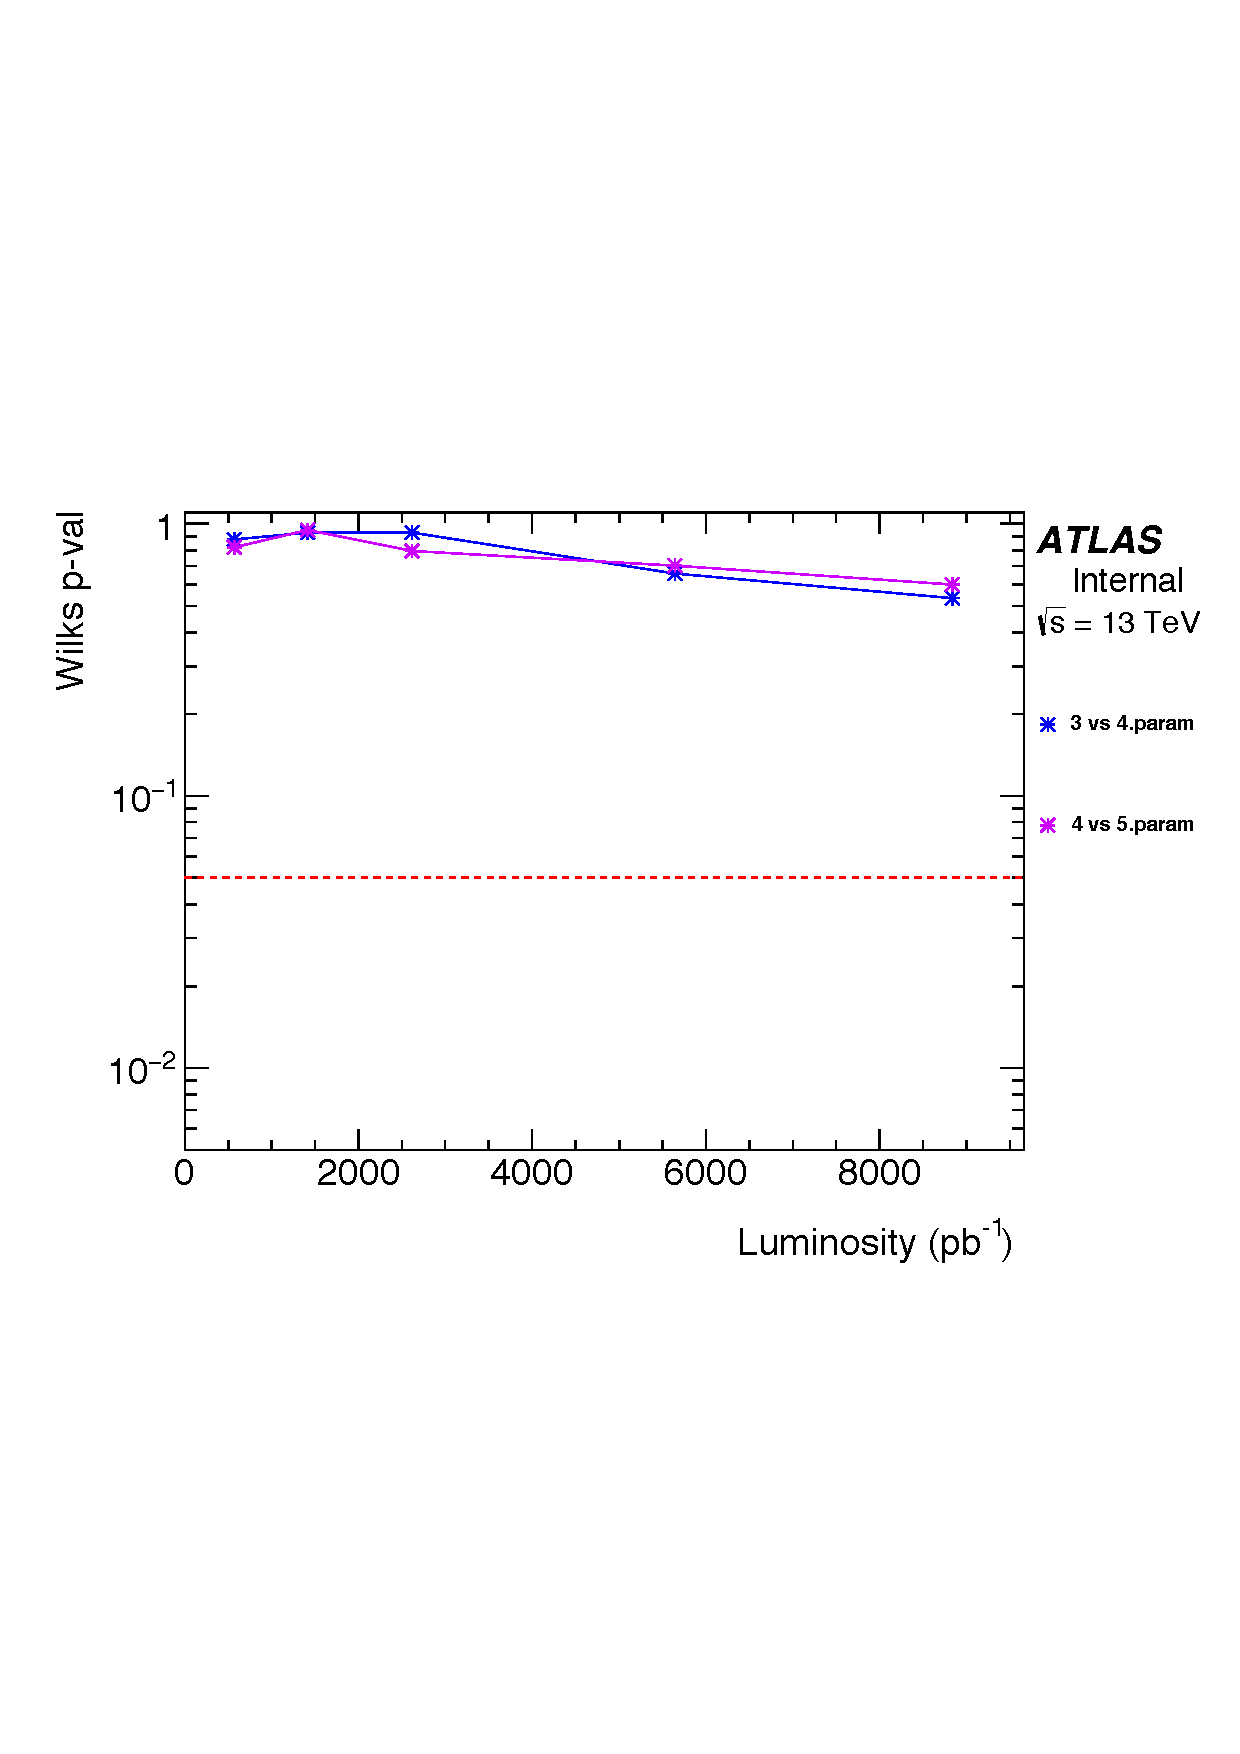
\includegraphics[width=0.47\linewidth, angle=0]{figs/Dibjet/ICHEP/bkg-WilksStat_bb.pdf}}
   \subcaptionbox{$\geq$1 $b$-tag}{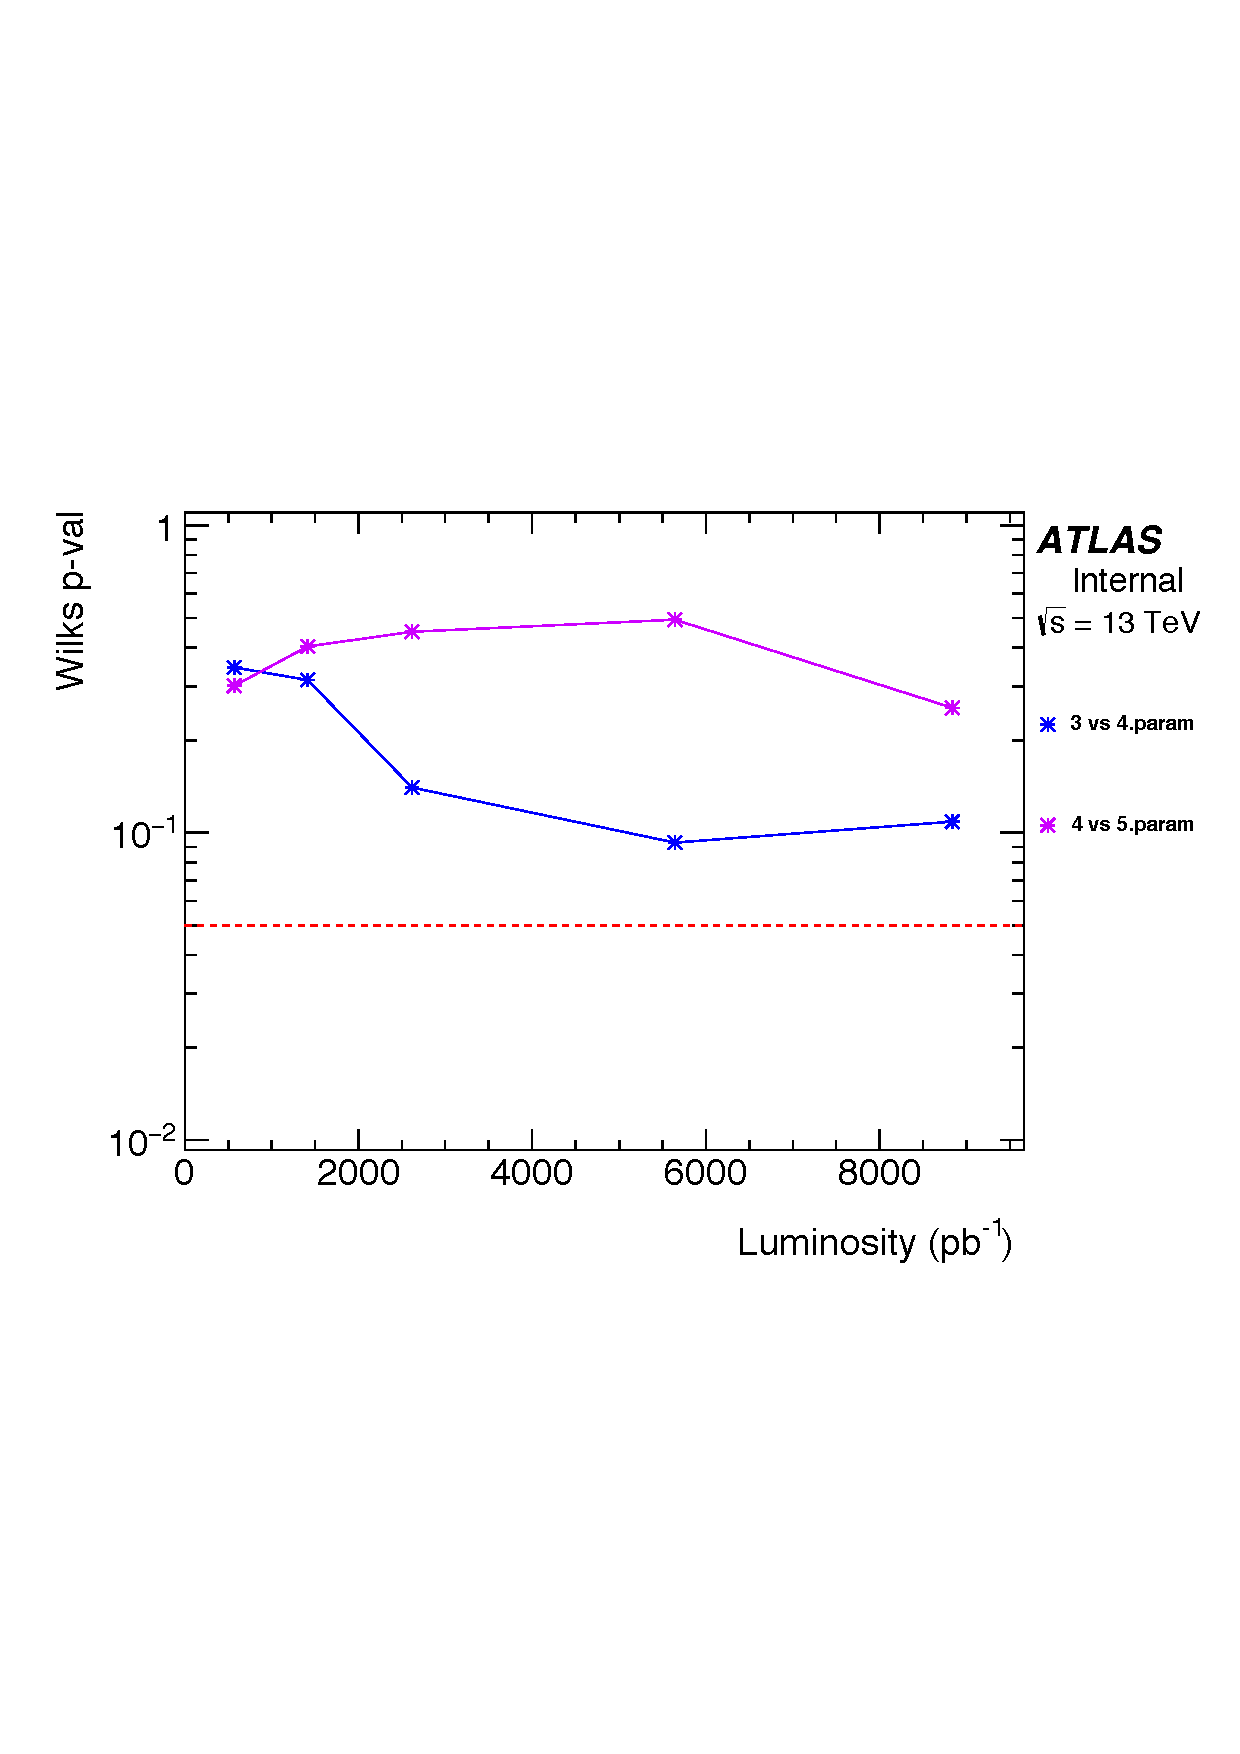
\includegraphics[width=0.47\linewidth, angle=0]{figs/Dibjet/ICHEP/bkg-WilksStat_b.pdf}}
  \end{center}
  \caption{The Wilks' $p$-value as a function of luminosity
    in the case that the 3 parameter is the nominal function and the 4 parameter is the alternate (blue)
    and the case where the 4 parameter is the nominal function and the 5 parameter is the alternate (purple)
    for the final data-set in the (a) 2 $b$-tag and (b) $\geq1$ $b$-tag category.
  }
  \label{fig:bkg-summer-wilks}
\end{figure}

\subsection{Fit Tests: Background-Only Dataset}
\label{sec:bkg-summer_fitCR}

To demonstrate that the dijet fit functions are a valid description of the background,
fit tests are peformed to a representative background only data-set.

To perform these tests, a {\sc pythia}8 MC multi-jet simulation is used as the representative background only data-set.
The simulation sample is produced in several slices of leading jet $p_{T}$, where each slice contains the same number of events.
A weight is applied to each event such that final distribution shape is representative of the smoothly falling~\mjj~spectrum that is expcted,
whilst still maintaining a similar precision across the full mass range.
The weighted invariant mass distribution is then scaled to 10~\ifb~\footnote{
  These studies were carried out during data-taking
  and as such the final integrated luminosity of the data-set had to be estimated,
  10~\ifb was used where the final data-set is 13.3~\ifb.
},
this is referred to as the  `scaled distribution', which can be interpretated as the expected number of data events in a specific mass bin. 
The precision of the scaled distribution is represented by the the number of `effective entries';
the number of effective entries is the number of data events that would be required to give the same precision,
or to put it another way it is the square of the error in that mass bin. The number of effective entries can be calculated from the event weights as shown in Equation~\ref{eq:effEnt}.
\begin{equation}
  N_{eff} = (\sum{w_i})^2 / \sum{w_i^2}
  \label{eq:effEnt}
\end{equation}
Figure~\ref{fig:effEnt} shows the scaled and effective entries distributions as a function of dijet invariant mass for the 2 $b$-tag and $\geq$1 $b$-tag categories. 

\begin{figure}[!ht]
  \begin{center}
    \captionsetup[subfigure]{aboveskip=0pt,justification=centering}
   \subcaptionbox{2 $b$-tag}{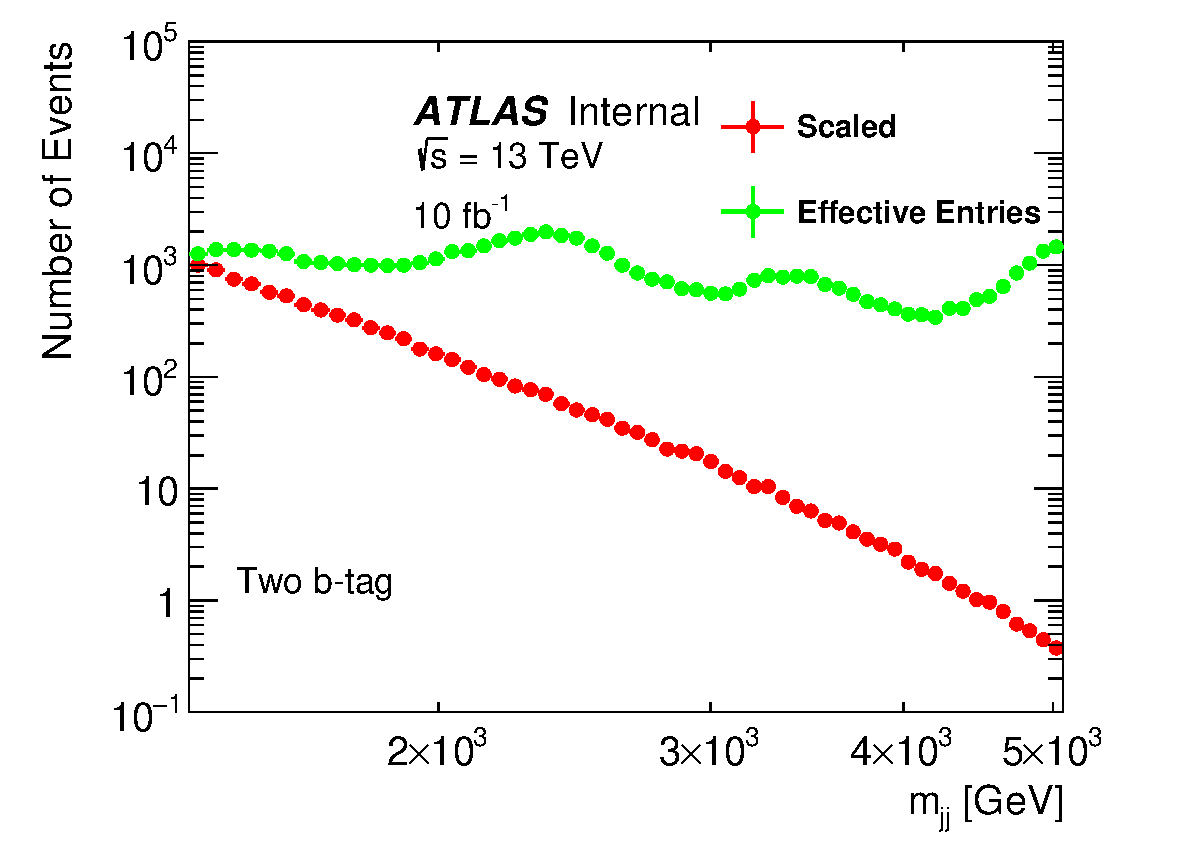
\includegraphics[width=0.47\linewidth, angle=0]{figs/Dibjet/ICHEP/FitRange/mbb_fix_8585_effEntries_Logx_10fb.pdf}}
   \subcaptionbox{$\geq$1 $b$-tag}{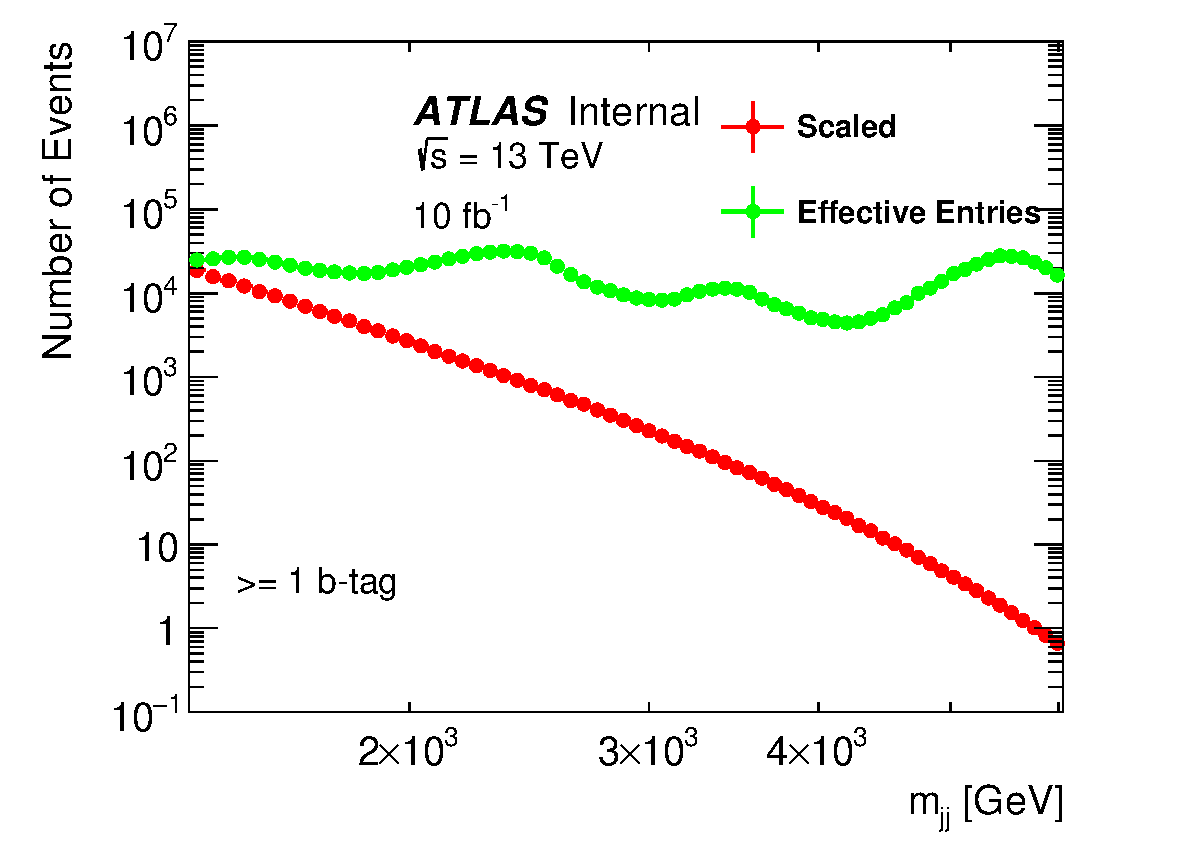
\includegraphics[width=0.47\linewidth, angle=0]{figs/Dibjet/ICHEP/FitRange/mbj_inc_fix_8585_effEntries_Logx_10fb.pdf}}
  \end{center}
  \caption{The scaled invariant mass distribution (red) compared to the
    effective entries of the invariant mass distribution (green)
    of Monte-Carlo simulation for the (a) 2 $b$-tag and (b) $\geq$1 $b$-tag category.
    The \textit{Summer16+15} dataset event selection has been applied.}
  \label{fig:effEnt}
\end{figure}

\subsection{Fit Tests: Mass Range Studies}
\label{sec:bkg-summer_range}

The first fit test is to demonstrate that
the dijet fit functions are able to describe the~\mjj~spectra.
In this test the scaled invariant mass spectra from simulation,
are fitted to using the search phase procedure.
The errors on the invariant mass spectrum
are given by the square root of the number of effective entries
which effectively gives the statistical error of the simulated sample.

The dijet mass spectra considered have a lower mass edge of $m_{jj}$ = 1100 GeV,
selected such that there is no kinematic bias from the single jet trigger,
and the upper edge is the mass bin at which the dijet mass spectrum goes below one entry per bin.
Figure~\ref{fig:Short_4para_1100_figure1} and \ref{fig:Short_5para_1100_figure1} show the search phase
for both $b$-tag categories, fitted to with the 4 and 5 parameter fit function.
The most discrepant excess is indicated by the blue lines and the BumpHunter $p$-value of the excess is shown on the plot,
which has been calculated using 10,000 pseudo-experiments.
Similarly, the $p$-value of the most discrepant deficit is calculated using the same process, which is referred to as DeficitHunter,
and an overall quality of fit $p$-value is also calculated by the same process using the $\chi^{2}$ test statistic.

For both fit functions in the $\geq$1 $b$-tag category,
a large excess is observed which has been assigned a BumpHunter $p$-value of 0.00.
This indicates that the 4 and 5 parameter fit functions
provide a poor description of the background distribution from simulation
in the $\geq1$ $b$-tag category.
Note that although these studies have been performed with the 4 and 5 parameter function,
as the 3 parameter function is a subset of the 4 parameter function it can also be concluded
that the 3 parameter function will also be inadquete.

\begin{figure}[!ht]
  \begin{center}
   \captionsetup[subfigure]{aboveskip=0pt,justification=centering}
   \subcaptionbox{2 $b$-tag}{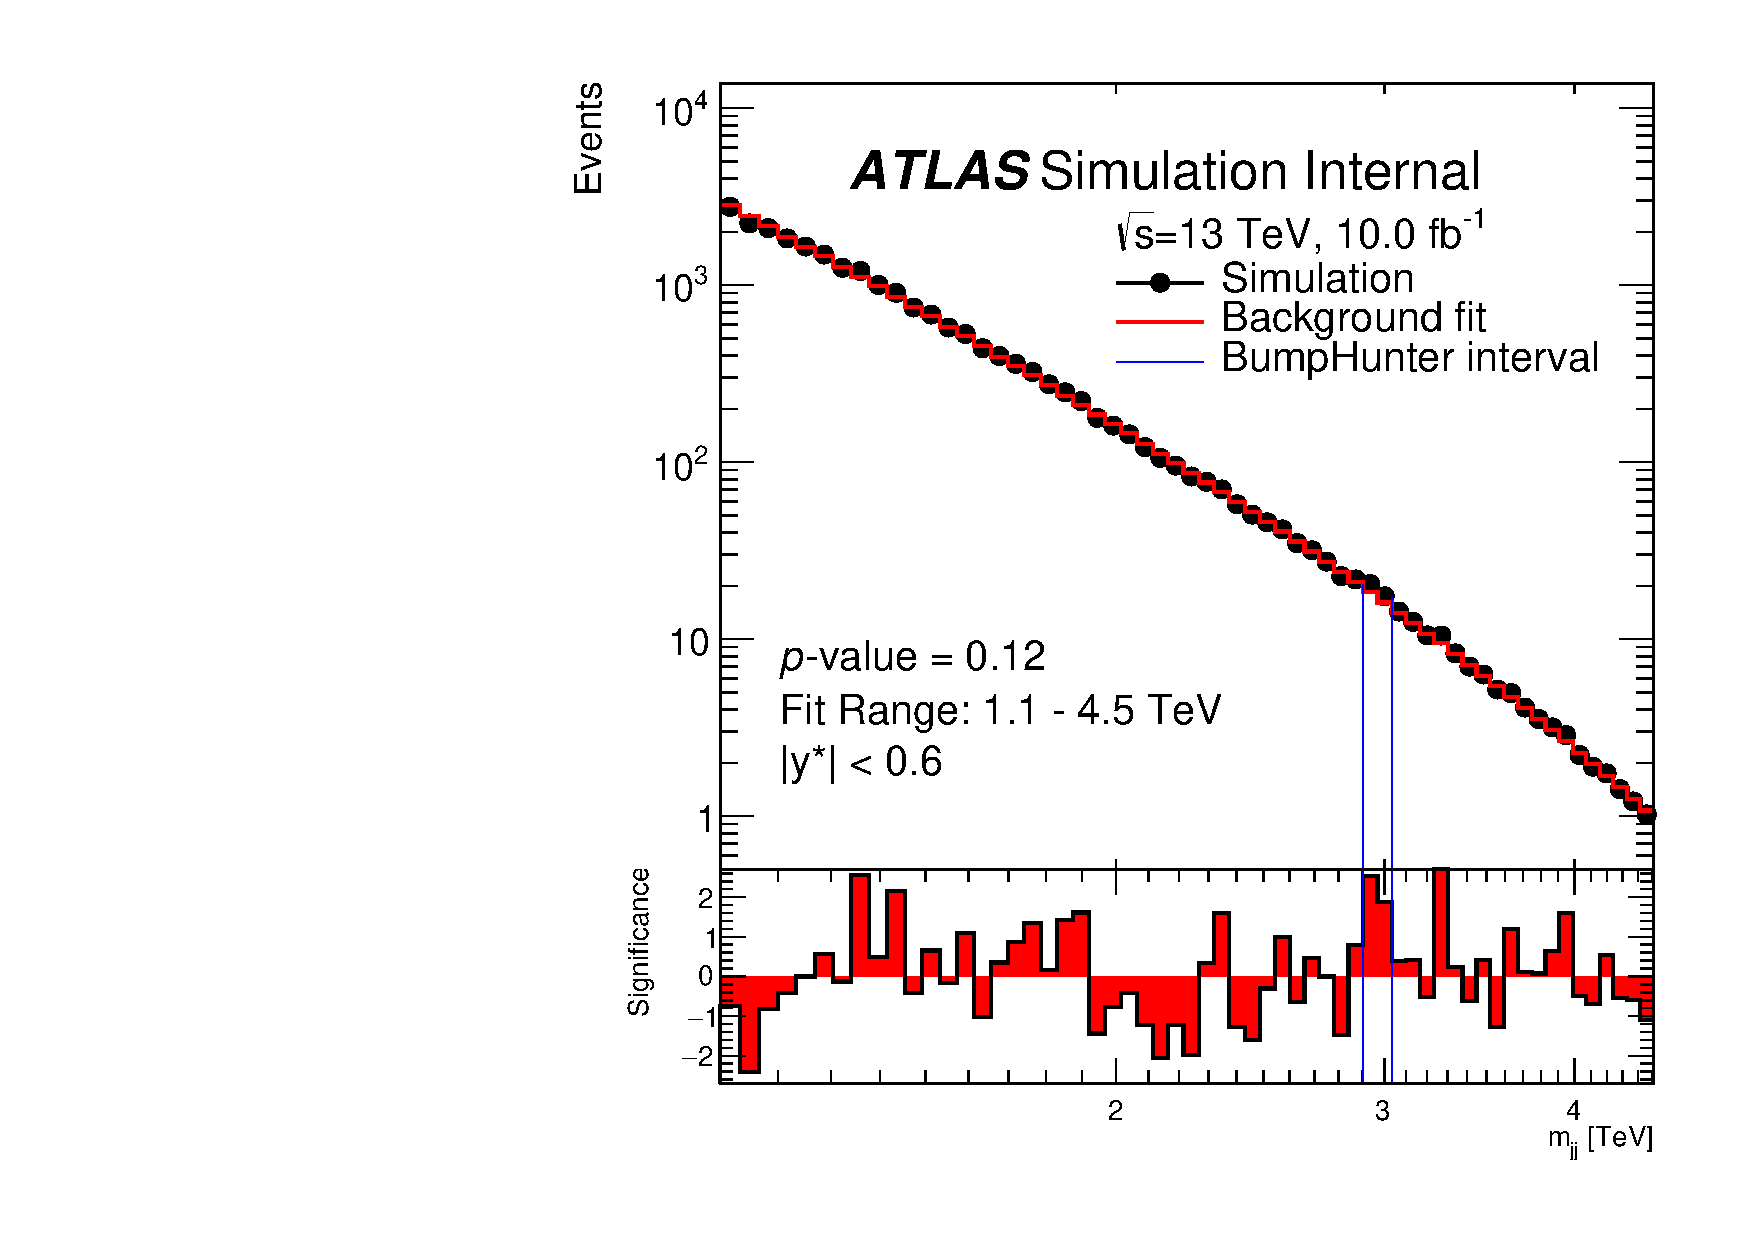
\includegraphics[width=0.47\linewidth, angle=0]{figs/Dibjet/ICHEP/FitRange/mbb_fix_8585_Short_4para_1100_figure1_10fb.pdf}}
   \subcaptionbox{$\geq$1 $b$-tag}{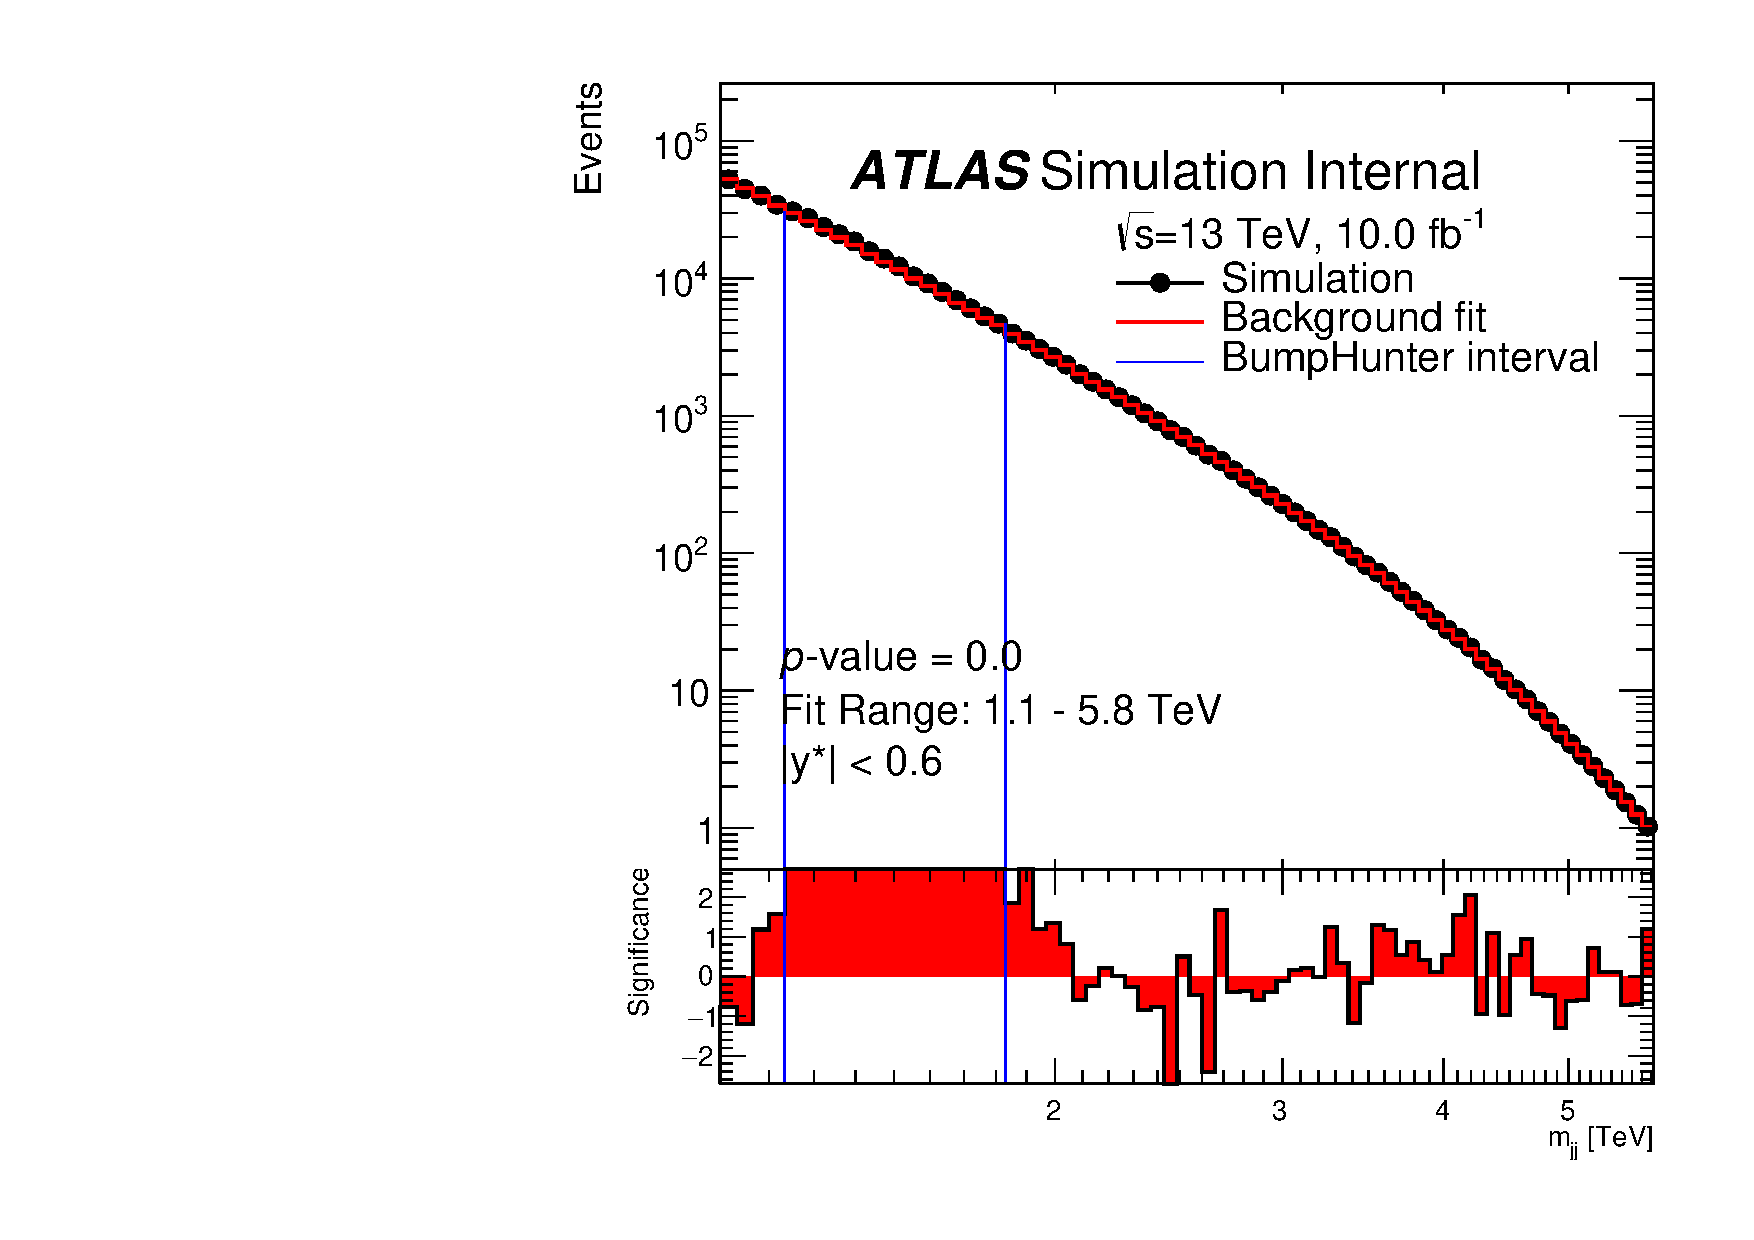
\includegraphics[width=0.47\linewidth, angle=0]{figs/Dibjet/ICHEP/FitRange/mbj_inc_fix_8585_Short_4para_1100_figure1_10fb.pdf}}
  \end{center}
  \caption{ The invariant mass distribution taken from multi-jet simulation for the (a) 2 $b$-tag and (b) $\geq$1 $b$-tag,
   category, fitted to using the 4 parameter fit function, with lower mass bound of the fit range $m_{jj}$ = 1100 GeV.
   The BumpHunter algorithm is run to identify the most discrepant excess, as indicated by the blue lines.
   Pseudo-experiments are used to assign the excess a $p$-value, which is shown on the plot.    
   The \textit{Summer16+15} dataset event selection has been applied.}
 \label{fig:Short_4para_1100_figure1}
\end{figure}


\begin{figure}[!ht]
  \begin{center}
    \captionsetup[subfigure]{aboveskip=0pt,justification=centering}
   \subcaptionbox{2 $b$-tag}{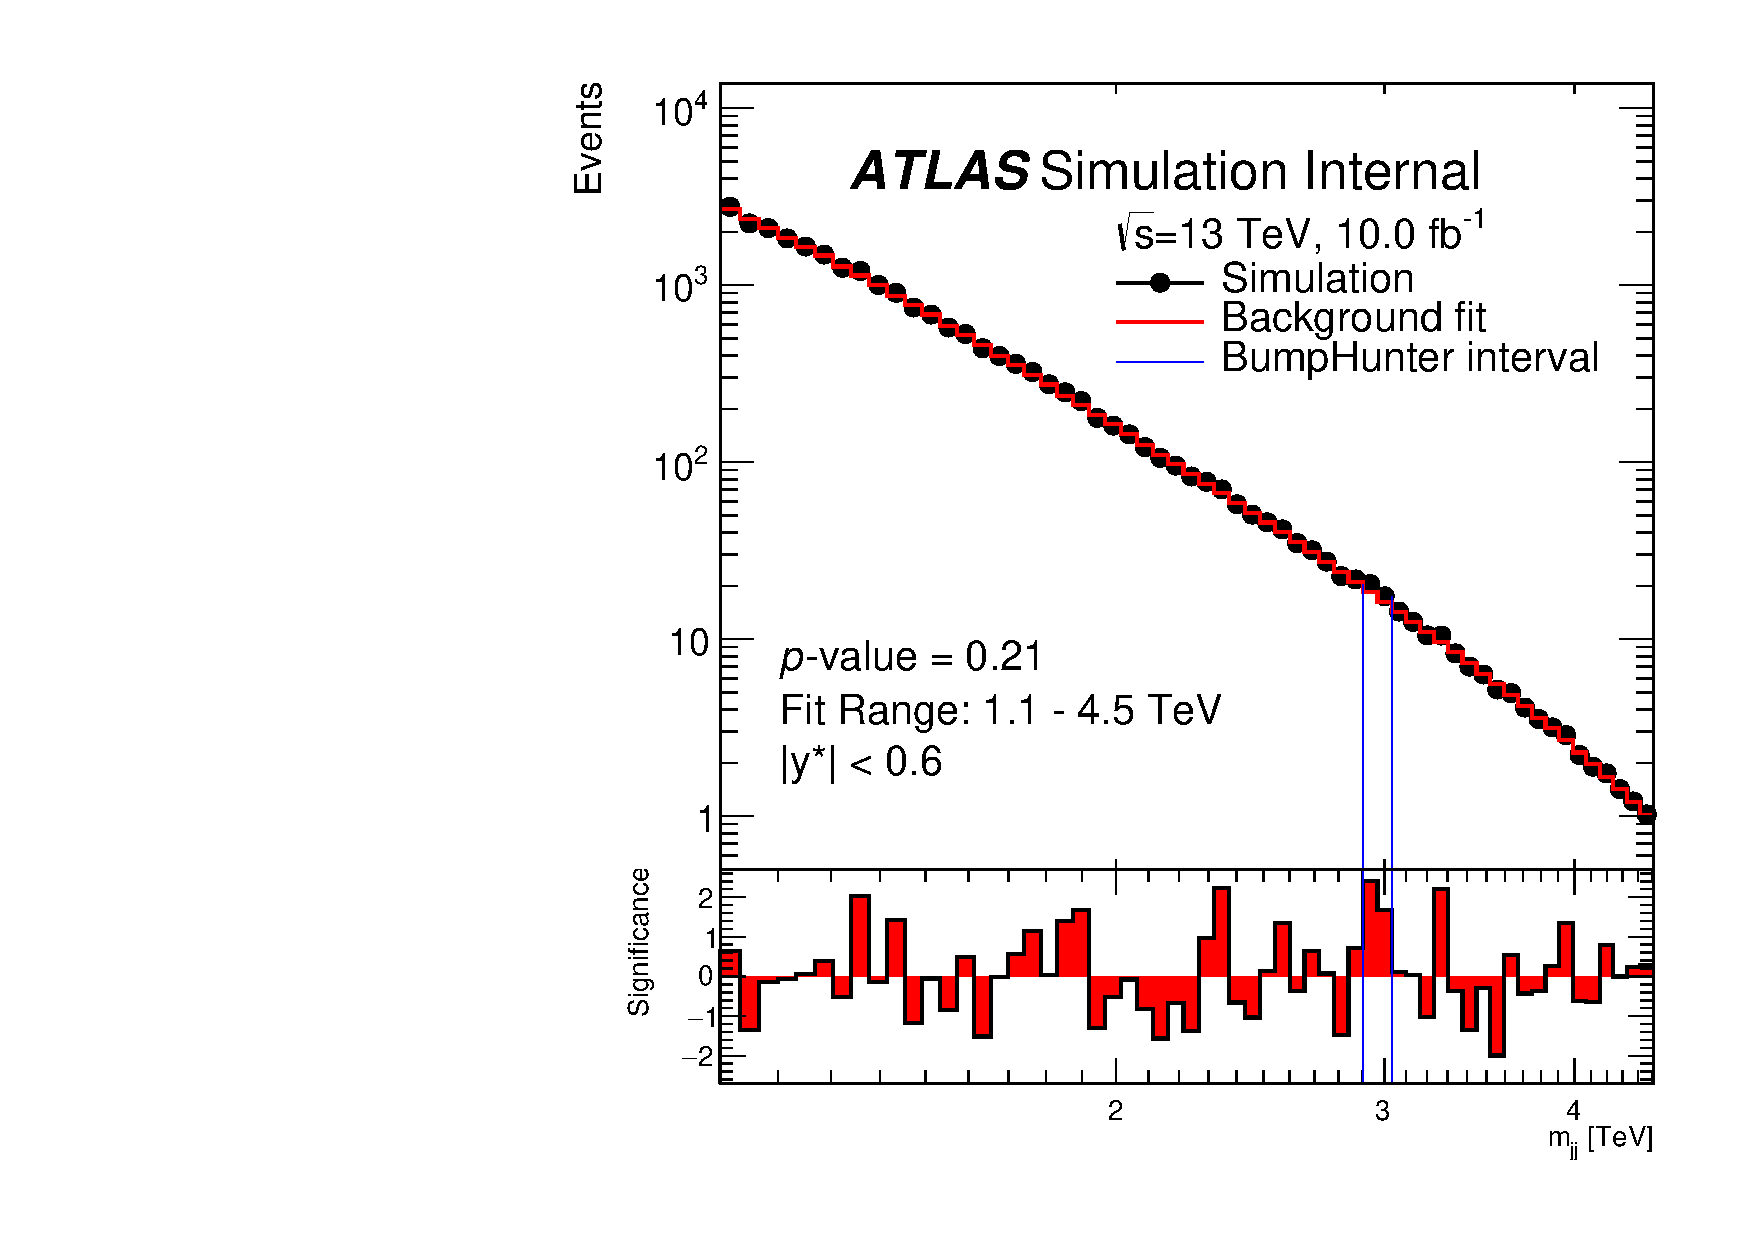
\includegraphics[width=0.47\linewidth, angle=0]{figs/Dibjet/ICHEP/FitRange/mbb_fix_8585_Short_5para_1100_figure1_10fb.pdf}}
   \subcaptionbox{$\geq$1 $b$-tag}{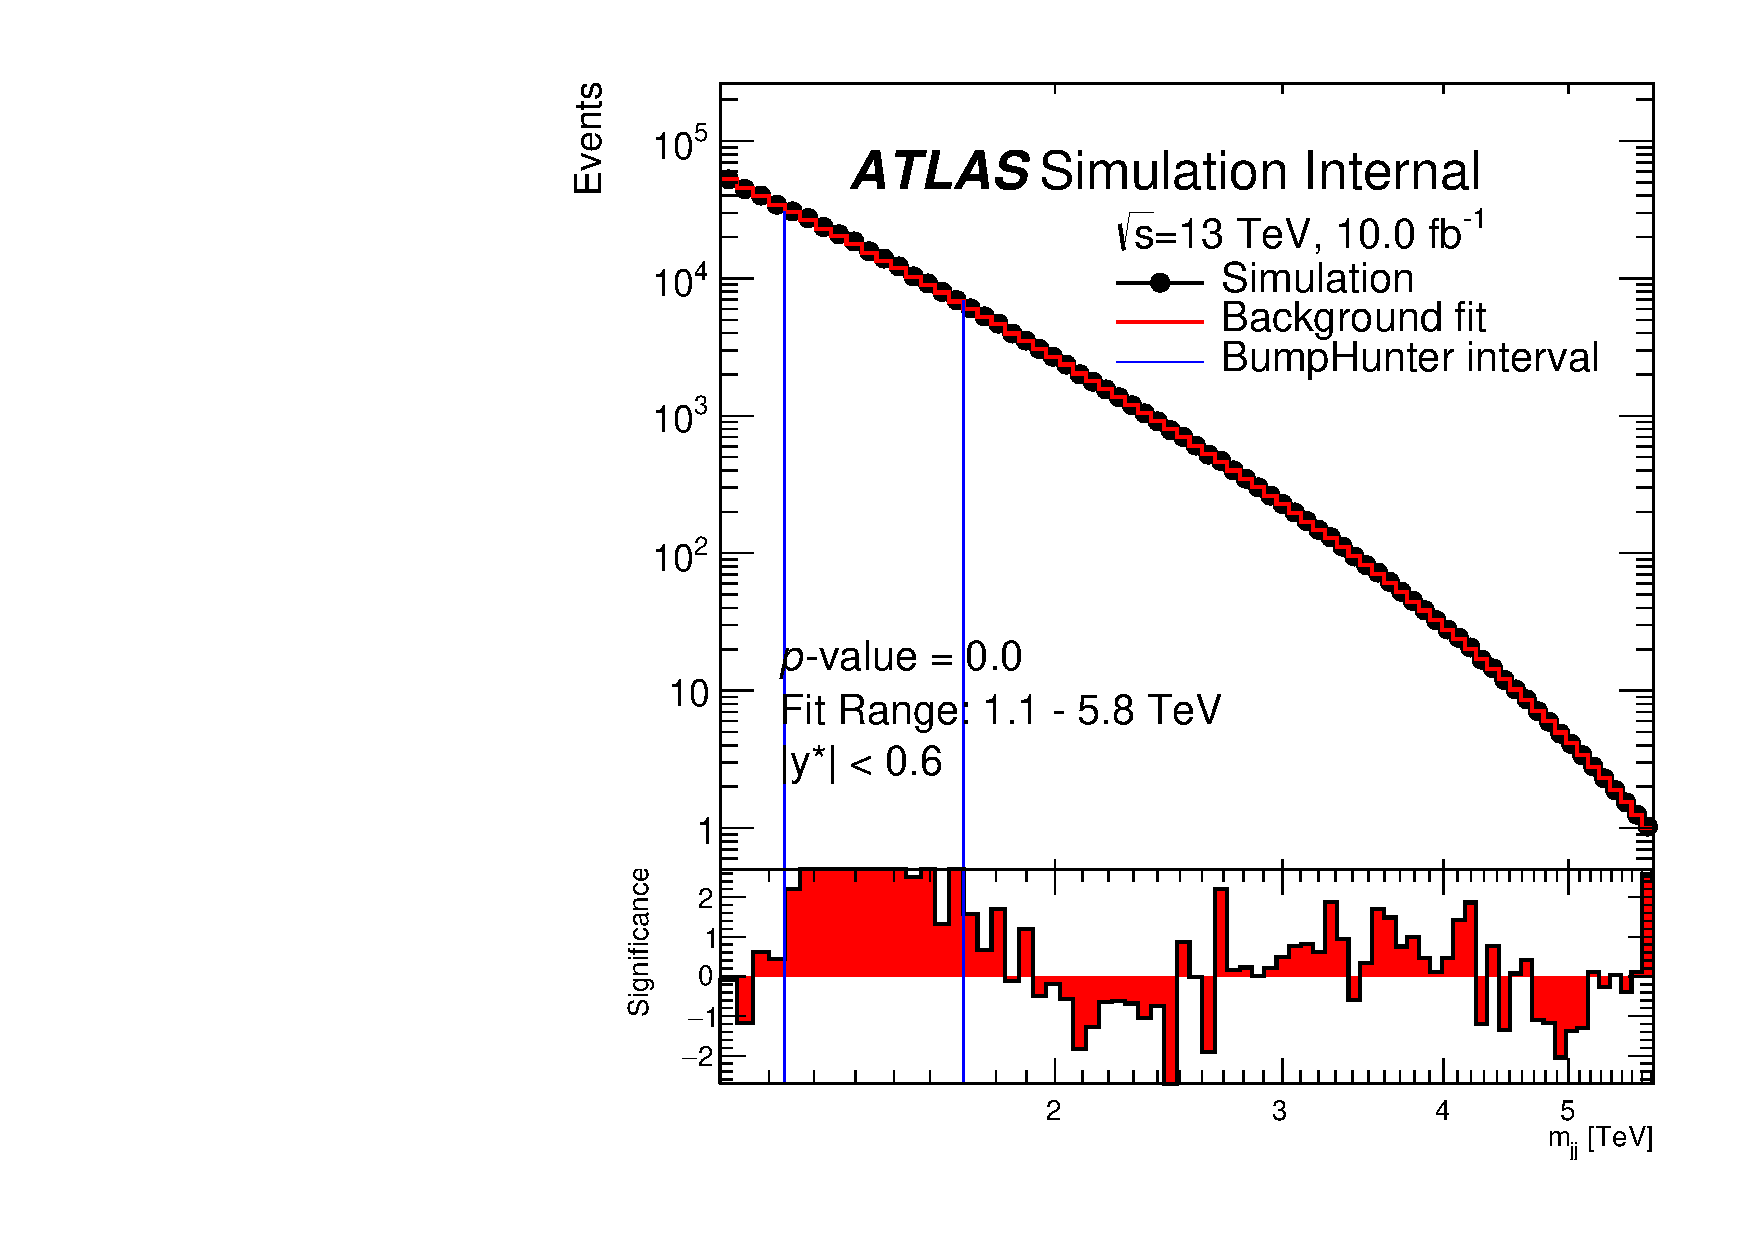
\includegraphics[width=0.47\linewidth, angle=0]{figs/Dibjet/ICHEP/FitRange/mbj_inc_fix_8585_Short_5para_1100_figure1_10fb.pdf}}
  \end{center}
  \caption{ The invariant mass distribution taken from multi-jet simulation for the (a) 2 $b$-tag and (b) $\geq$1 $b$-tag,
    category, fitted to using the 5 parameter fit function, with lower mass bound of the fit range $m_{jj}$ = 1100 GeV.
    The BumpHunter algorithm is run to identify the most discrepant excess, as indicated by the blue lines.
    Pseudo-experiments are used to assign the excess a $p$-value, which is shown on the plot.
    The \textit{Summer16+15} dataset event selection has been applied.}
  \label{fig:Short_5para_1100_figure1}
\end{figure}

\FloatBarrier

However, by changing the lower mass bound of the fit,
a region can be found where the fit functions are able to describe the background accurately.
To find the largest region with a stable fit quality, the simulated dijet mass spectrum is
fitted to using the 4 parameter function with the lower mass bound of the fit region increased one bin at a time,
beginning at $m_{jj}$ = 1100 GeV up to $m_{jj}$ = 1500 GeV.
As before the upper edge of the fit region is the mass bin at which the simulation goes below one entry per bin.
Figure~\ref{fig:mjjGraphs_bb} and \ref{fig:mjjGraphs_bj_inc} show,
for the 2 $b$-tag and $\geq1$ $b$-tag categories, the distributions of the
(a) BumpHunter, (b) DeficitHunter and (c) $\chi^{2}$ $p$-values as the lower mass bound of the fit region is increased.
In both categories it is shown that there are fit regions that are stable if the lower mass bound is $m_{jj}$ = 1378 GeV or above.
This demonstrates that there are features in the background mass spectrum at low masses that are causing a poor fit quality,
which can be removed by using a fit region $m_{jj} >$ 1378 GeV. 

Figure~\ref{fig:Short_4para_1378_figure1} shows the search phase applied to the dijet mass spectra
of the simulated sample for both $b$-tagging categories,
for the fit range with the lower mass bound of $m_{jj}$ = 1378 GeV,
fitted to using the 4 parameter fit function.
The most discrepant excess, as found by the BumpHunter algorithm, is indicated by the blue lines
and the $p$-value of the excess is shown on the plot.
This shows that the fit quality is reasonable for this choice of fit region.
The study presented in this section motivates the choice of $m_{jj} >$ 1378 GeV
as the lower mass cut used in the \verb|Summer16+15| data-set event selection.

\begin{figure}[!htb]
  \begin{center}
    \captionsetup[subfigure]{aboveskip=0pt,justification=centering}
    \subcaptionbox{BumpHunter}{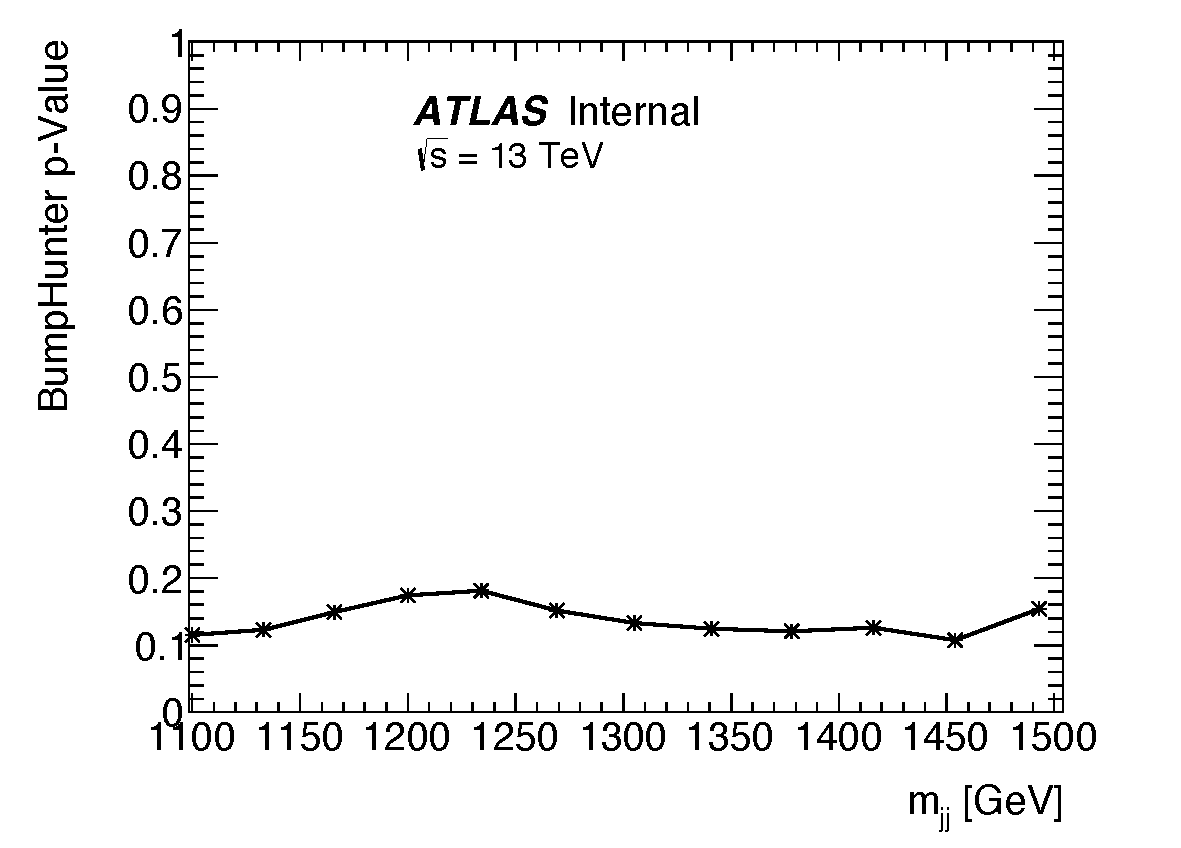
\includegraphics[width=0.325\linewidth, angle=0]{figs/Dibjet/ICHEP/FitRange/mbb_fix_8585_mjjGraph_bumpHunter_10fb.pdf}}
    \subcaptionbox{DeficitHunter}{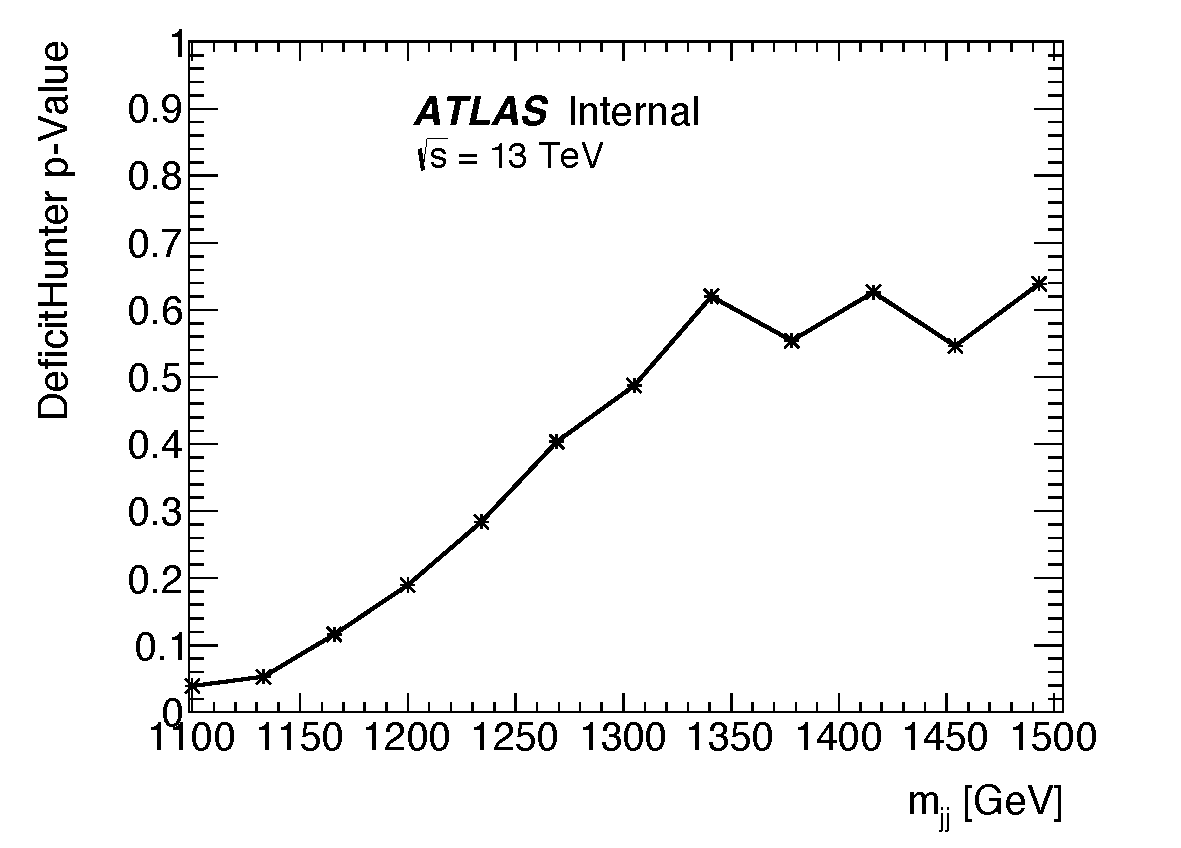
\includegraphics[width=0.325\linewidth, angle=0]{figs/Dibjet/ICHEP/FitRange/mbb_fix_8585_mjjGraph_deficitOnlyHunter_10fb.pdf}}
    \subcaptionbox{$\chi^{2}$}{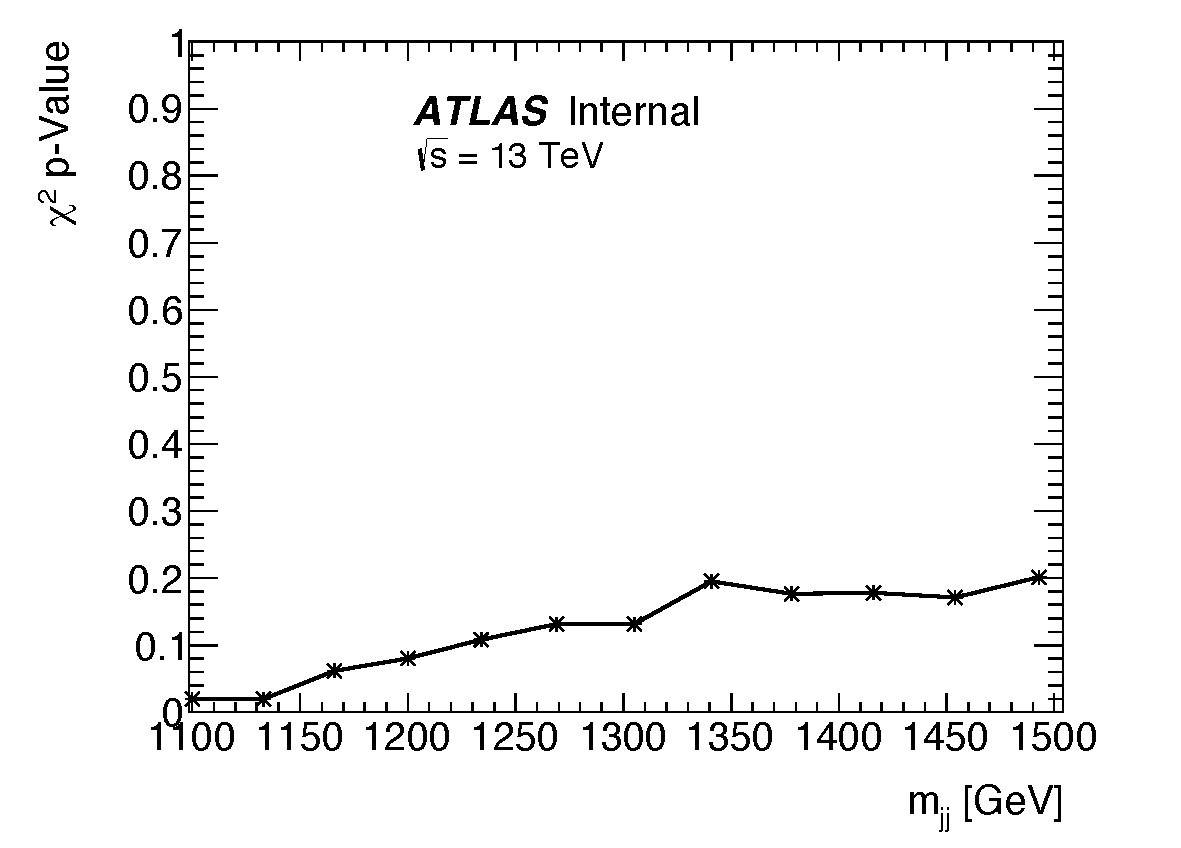
\includegraphics[width=0.325\linewidth, angle=0]{figs/Dibjet/ICHEP/FitRange/mbb_fix_8585_mjjGraph_chi2_10fb.pdf}}
  \end{center}
  \caption{The distribution of the (a) BumpHunter, (b) DeficitHunter and (c) $\chi^{2}$ $p$-values
    for different values of lower mass bound of the fit range, when fitting to 2 $b$-tag category
    invariant mass distribution taken from multi-jet simulation with the 4 parameter fit function.
    The \textit{Summer16+15} dataset event selection has been applied, with the exception of the~\mjj~cut.}
  \label{fig:mjjGraphs_bb}
\end{figure}

\begin{figure}[!htb]
  \begin{center}
    \captionsetup[subfigure]{aboveskip=0pt,justification=centering}
    \subcaptionbox{BumpHunter}{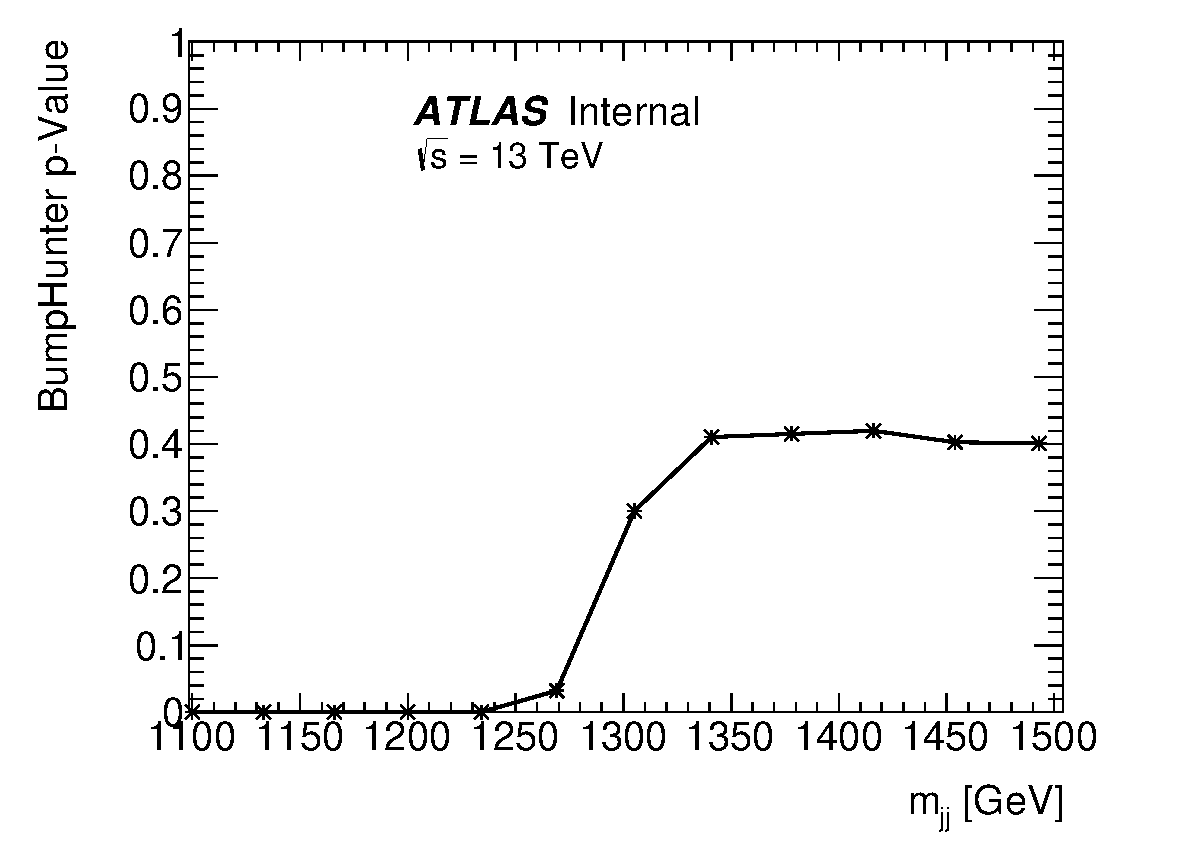
\includegraphics[width=0.325\linewidth, angle=0]{figs/Dibjet/ICHEP/FitRange/mbj_inc_fix_8585_mjjGraph_bumpHunter_10fb.pdf}}
    \subcaptionbox{DeficitHunter}{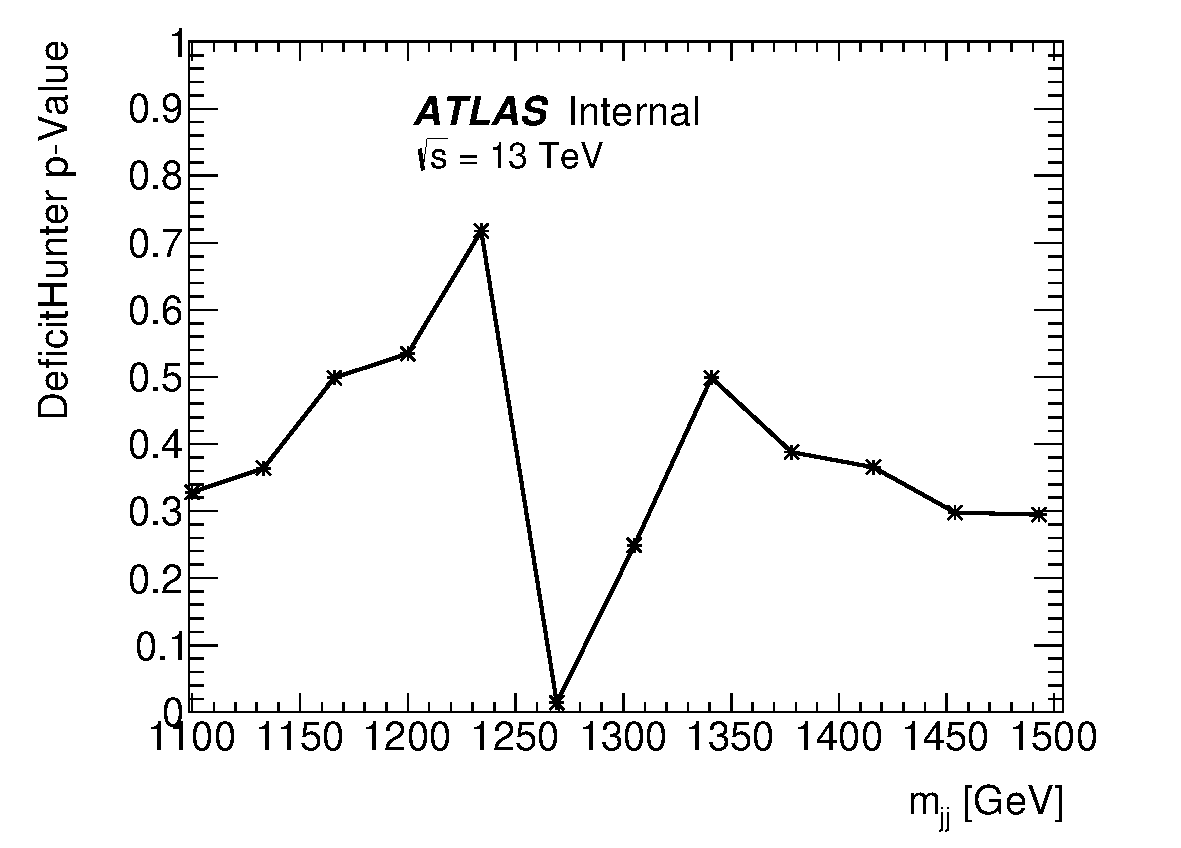
\includegraphics[width=0.325\linewidth, angle=0]{figs/Dibjet/ICHEP/FitRange/mbj_inc_fix_8585_mjjGraph_deficitOnlyHunter_10fb.pdf}}
    \subcaptionbox{$\chi^{2}$}{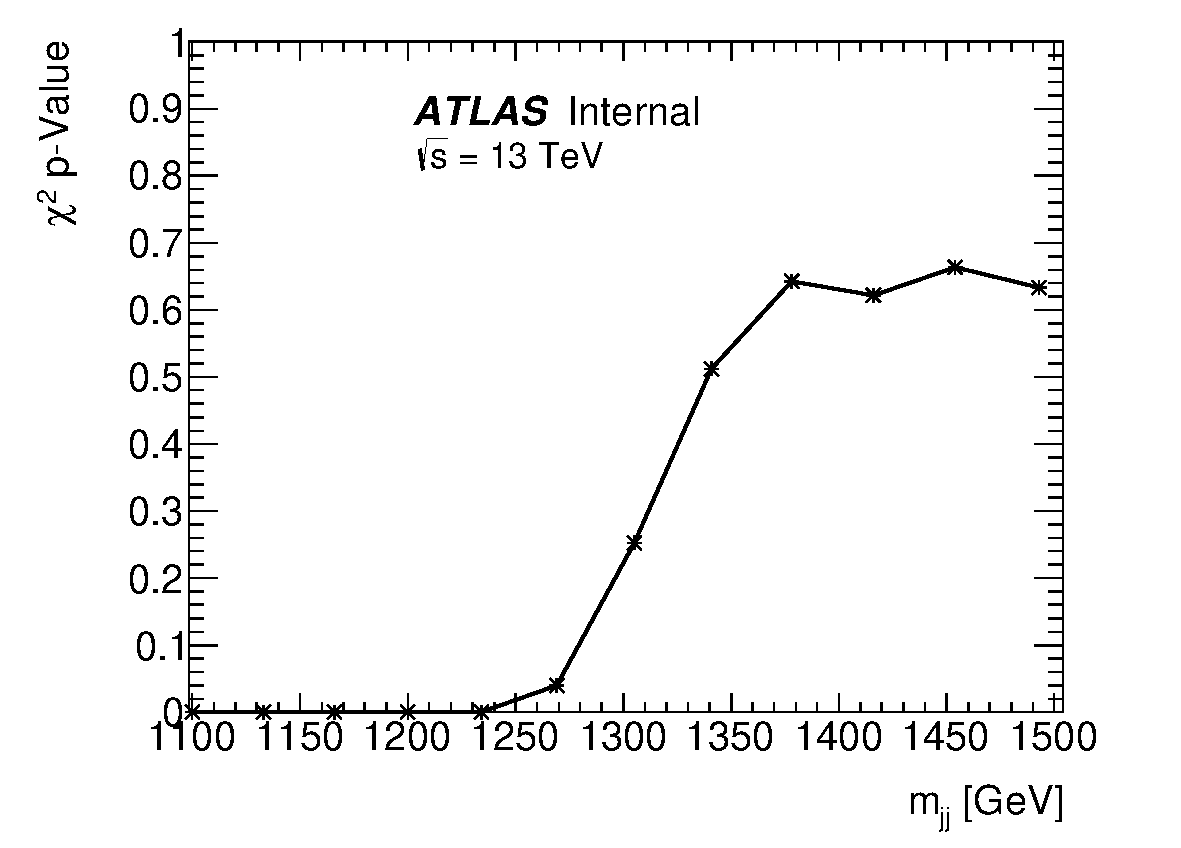
\includegraphics[width=0.325\linewidth, angle=0]{figs/Dibjet/ICHEP/FitRange/mbj_inc_fix_8585_mjjGraph_chi2_10fb.pdf}}
  \end{center}
  \caption{The distribution of the (a) BumpHunter, (b) DeficitHunter and (c) $\chi^{2}$ $p$-values
    for different values of lower mass bound of the fit range, when fitting to $\geq$1 $b$-tag category
    invariant mass distribution taken from multi-jet simulation with the 4 parameter fit function.
    The \textit{Summer16+15} dataset event selection has been applied, with the exception of the~\mjj~cut.}
  \label{fig:mjjGraphs_bj_inc}
\end{figure}

\begin{figure}[!ht]
  \begin{center}
    \captionsetup[subfigure]{aboveskip=0pt,justification=centering}
   \subcaptionbox{2 $b$-tag}{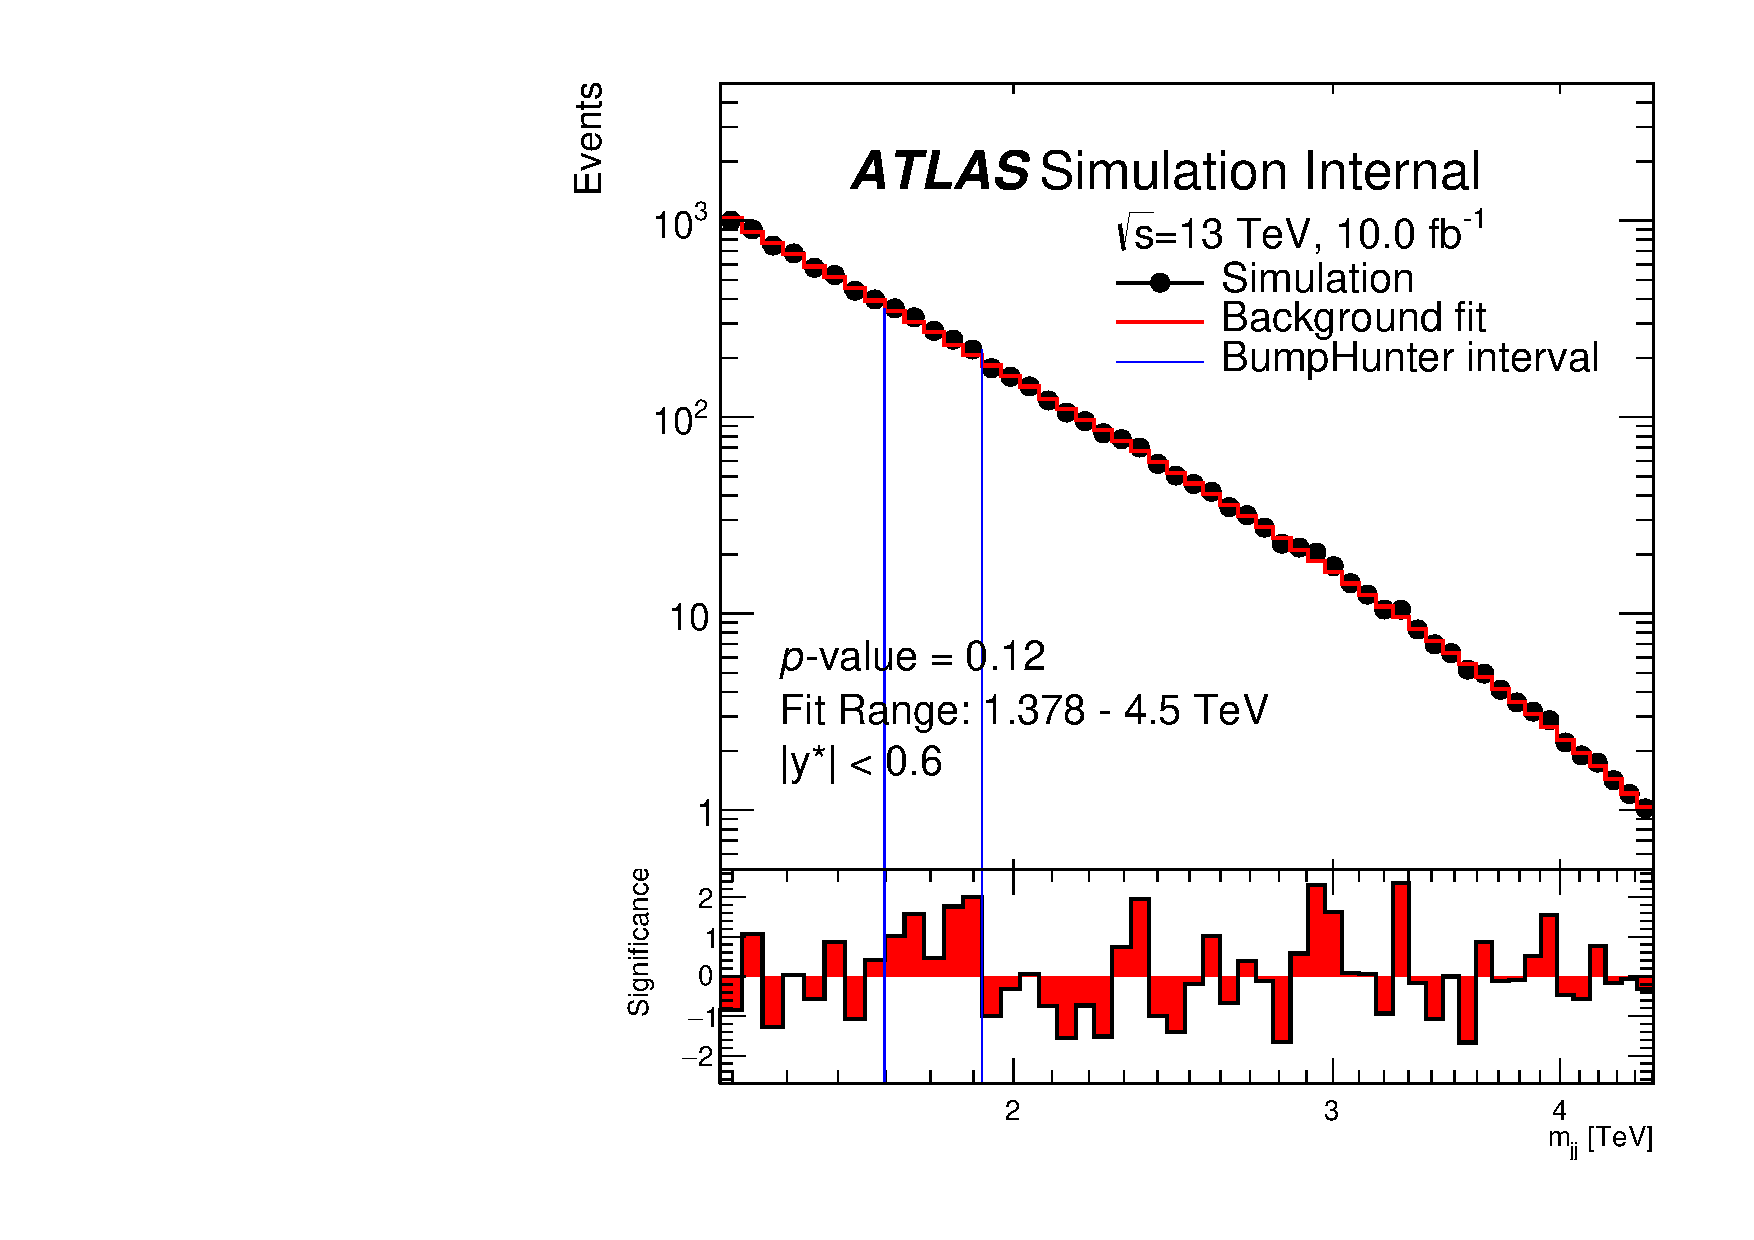
\includegraphics[width=0.47\linewidth, angle=0]{figs/Dibjet/ICHEP/FitRange/mbb_fix_8585_Short_4para_1378_figure1_10fb.pdf}}
   \subcaptionbox{$\geq$1 $b$-tag}{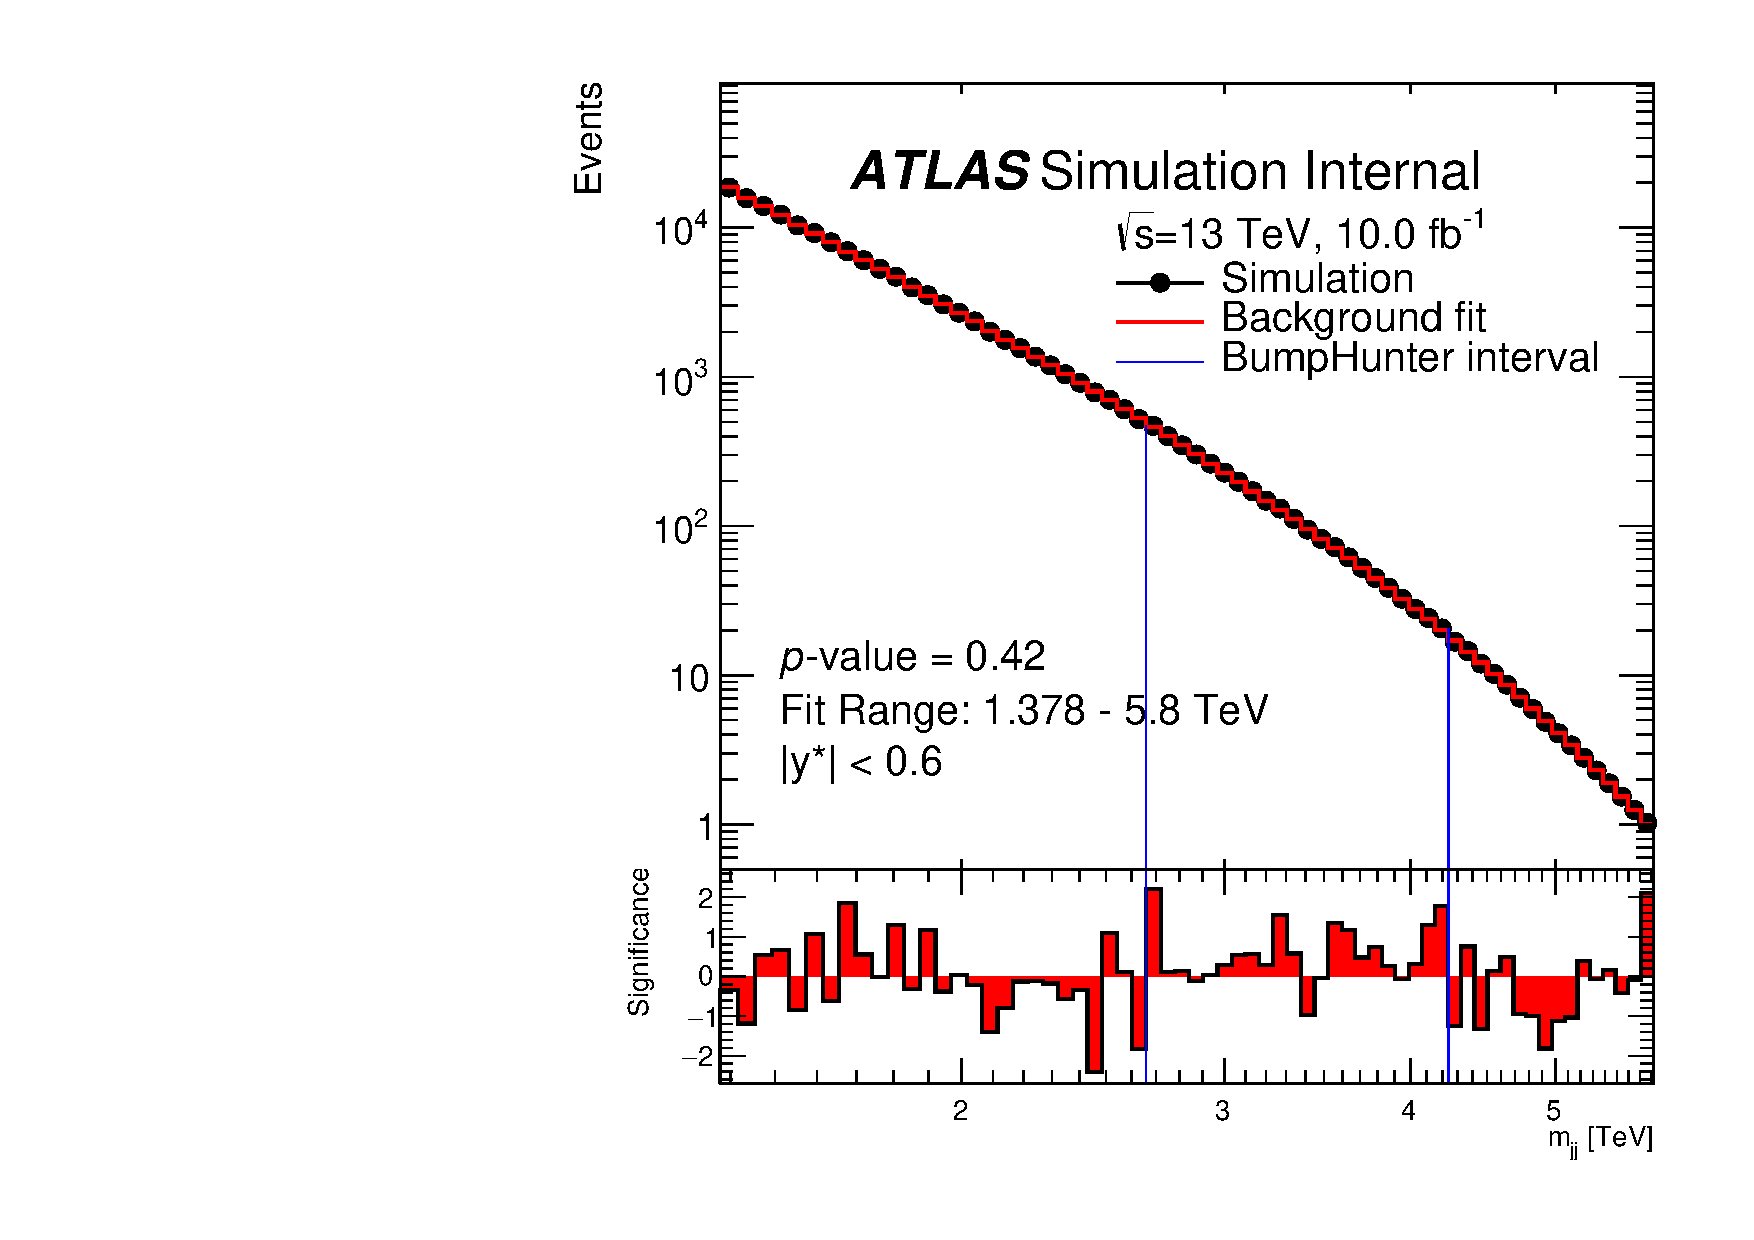
\includegraphics[width=0.47\linewidth, angle=0]{figs/Dibjet/ICHEP/FitRange/mbj_inc_fix_8585_Short_4para_1378_figure1_10fb.pdf}}
  \end{center}
  \caption{ The invariant mass distribution taken from multi-jet simulation for the (a) 2 $b$-tag and (b) $\geq$1 $b$-tag,
    category, fitted to using the 4 parameter fit function, with lower mass bound of the fit range $m_{jj}$ = 1378 GeV.
    The BumpHunter algorithm is run to identify the most discrepant excess, as indicated by the blue lines.
    Pseudo-experiments are used to assign the excess a $p$-value, which is shown on the plot. 
    The \textit{Summer16+15} dataset event selection has been applied.}
  \label{fig:Short_4para_1378_figure1}
\end{figure}

%\begin{figure}[!ht]
%  \begin{center}
%    \captionsetup[subfigure]{aboveskip=0pt,justification=centering}
%   \subcaptionbox{2 $b$-tag}{
%      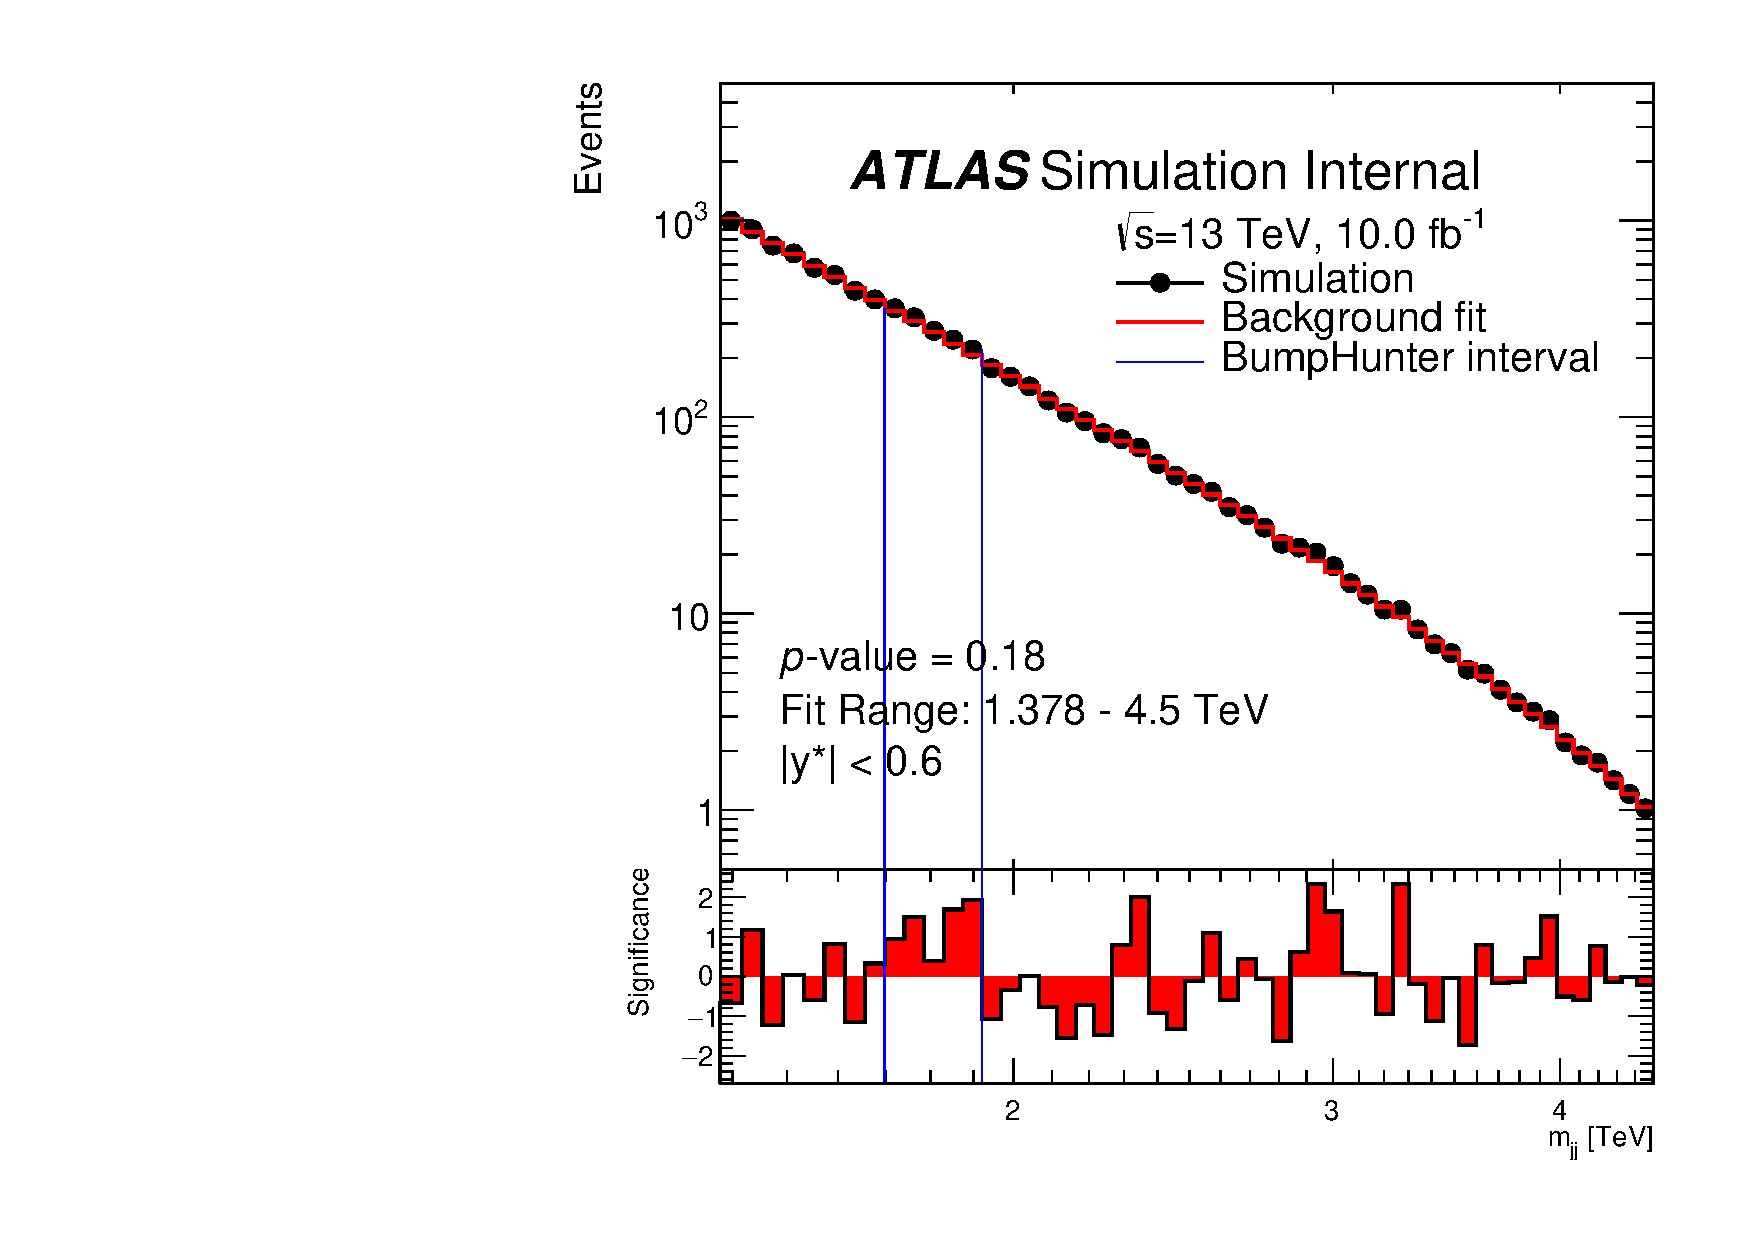
\includegraphics[width=0.47\linewidth, angle=0]{figs/Dibjet/ICHEP/FitRange/mbb_fix_8585_Short_5para_1378_figure1_10fb.pdf}
%    }
%   \subcaptionbox{$\geq$1 $b$-tag}{
%      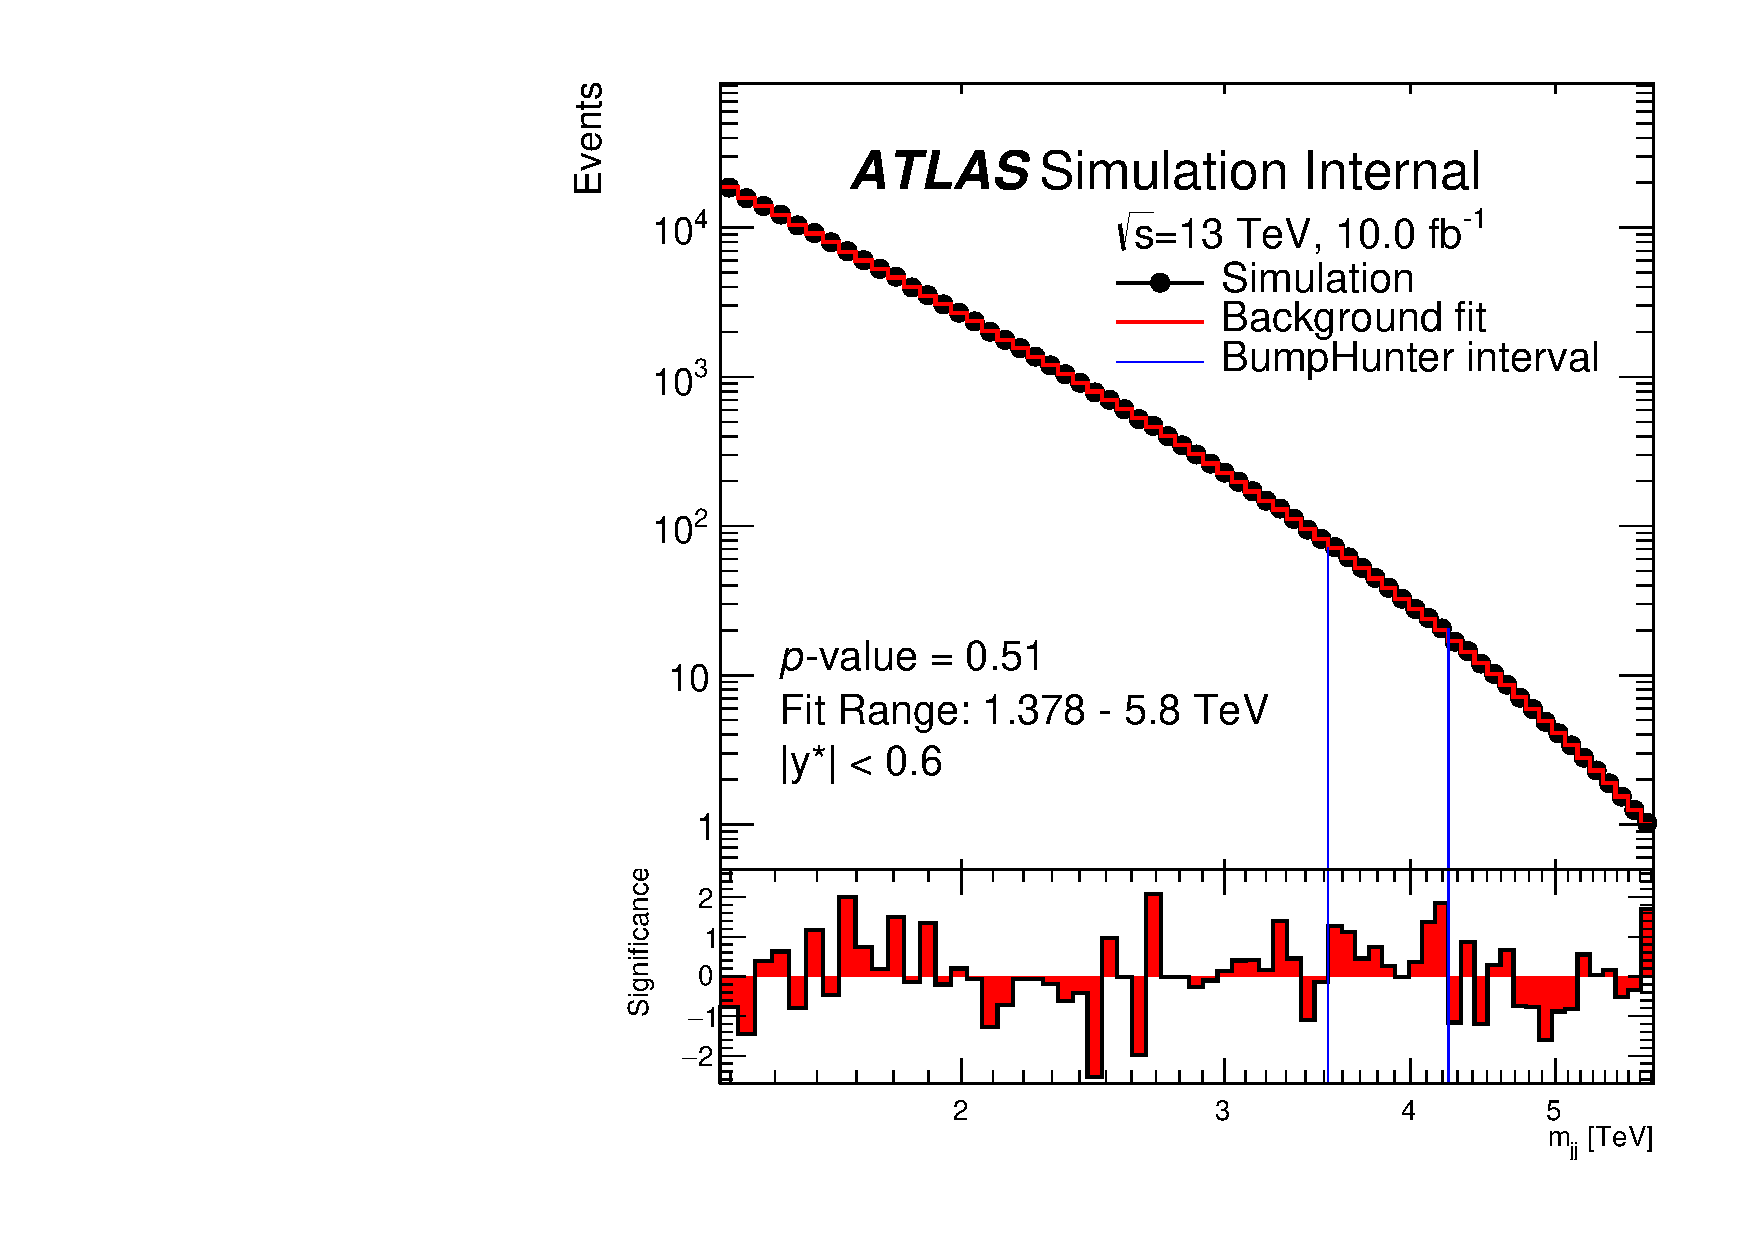
\includegraphics[width=0.47\linewidth, angle=0]{figs/Dibjet/ICHEP/FitRange/mbj_inc_fix_8585_Short_5para_1378_figure1_10fb.pdf}
%    }
%  \end{center}
%  \caption{ for the (a) 2 $b$-tag and (b) $\geq$1 $b$-tag category.}
%  \label{fig:}
%\end{figure}


\subsection{Fit Tests: Spurious Signal}
\label{sec:bkg-summer_spusig}

If the true background dijet invariant mass spectrum cannot be described by the chosen fit function,
then fit discrepancies can occur that could appear as false signal or could hide a true signal,
the former is referred to as spurious signal.
To show that fit discrepancies are not occuring, fits are peformed to a background-only representative data-set
to demonstrate that the chosen fit function is a valid representation of the true background spectrum.
Similar tests have been performed in previous iterations of both the inclusive and $b$-tagged dijet searches~\cite{dijet-mori16_paper,dibjet-mori16_paper}.

To perform these tests, the scaled distribtuion from the {\sc pythia}8 Monte-Carlo multi-jet simulation
described in Section~\ref{sec:bkg-summer_fitCR}
is used as the representative background only data-set.
%In Section~\ref{sec:FitStudies:FitRegion}
%the dijet mass spectrum used took the square root of the
%number of effective entries as the errors.
As shown in Figure~\ref{fig:effEnt},
the number of effective entries is larger than the number of scaled entries,
meaning that the distribution contains smaller statistical fluctuations than are present in the final data-set.
To create a more representative simulated data-set to test the fit functions,
Poisson fluctuations are applied to the scaled distribution to create a `data-like' distribution.
Figure~\ref{fig:effEntDataLike} shows the scaled and effective entries distributions for both
$b$-tag categories overlaid with a data-like distribution in blue.

\begin{figure}[!ht]
  \begin{center}
   \captionsetup[subfigure]{aboveskip=0pt,justification=centering}
    \subcaptionbox{2 $b$-tag}{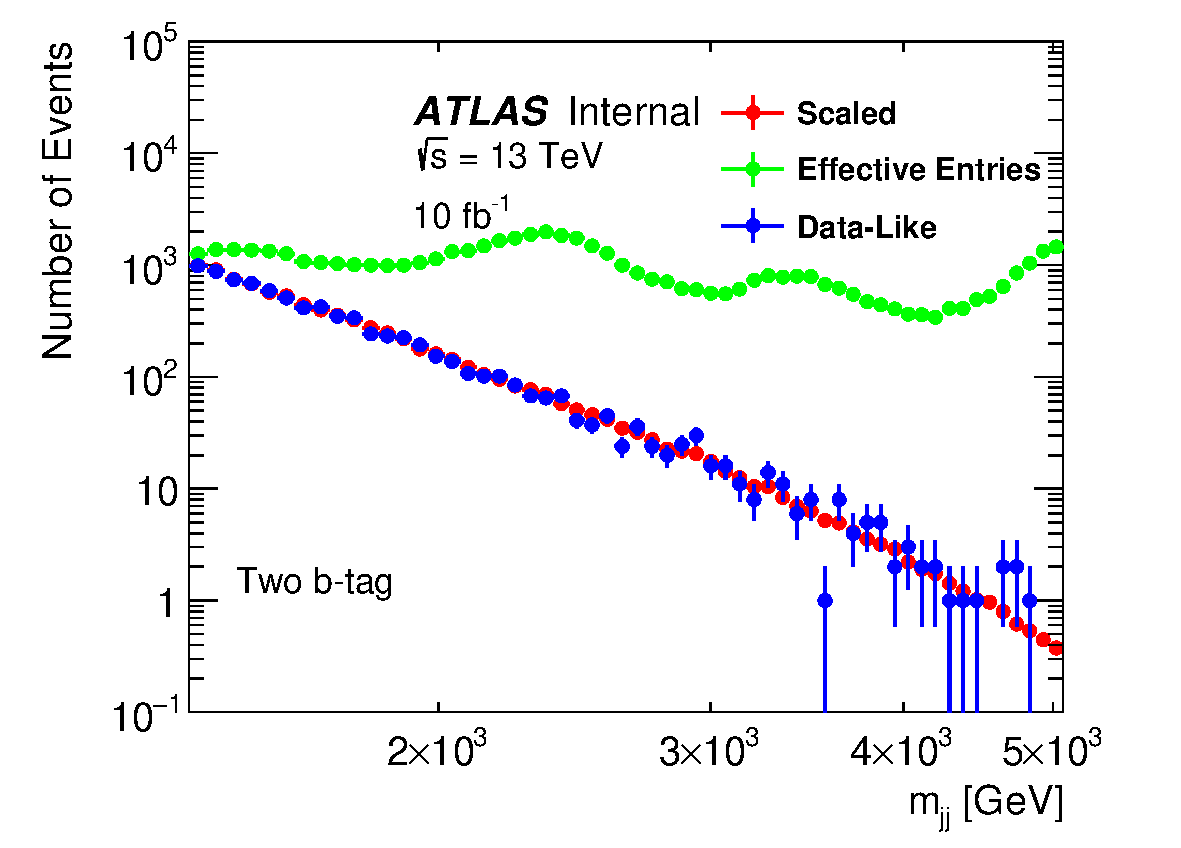
\includegraphics[width=0.47\linewidth, angle=0]{figs/Dibjet/ICHEP/SpuriousSignal/mbb_fix_8585_dataLike_effEntries_Logx_10fb.pdf}\label{fig:effEntDataLike_bb}}
    \subcaptionbox{$\geq$1 $b$-tag}{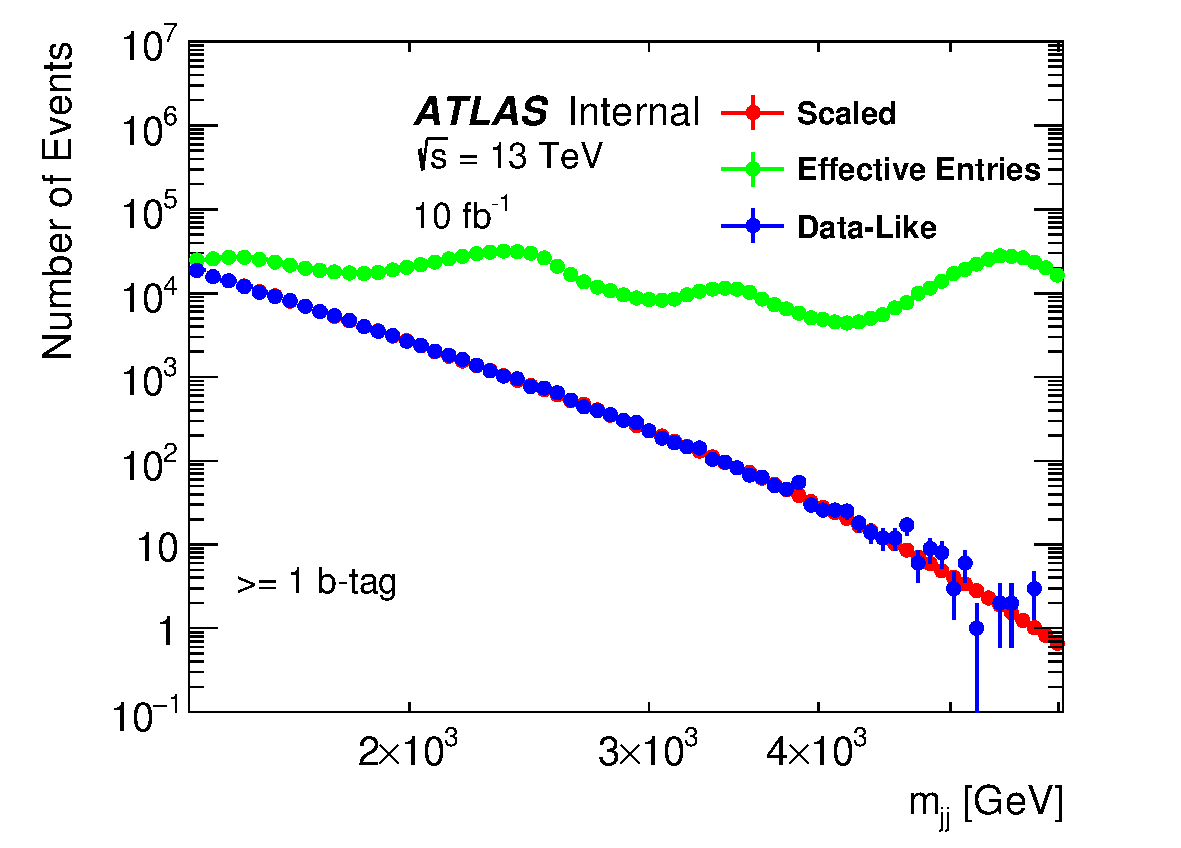
\includegraphics[width=0.47\linewidth, angle=0]{figs/Dibjet/ICHEP/SpuriousSignal/mbj_inc_fix_8585_dataLike_effEntries_Logx_10fb.pdf}\label{fig:effEntDataLike_bj}}
  \end{center}
  \caption{The scaled invariant mass distribution (red) compared to the
    effective entries of the invariant mass distribution (green) for the 2 $b$-tag category,
    for the (a) 2 $b$-tag and (b) $\geq$1 $b$-tag case.
    Overlaid is a data-like distribution (blue) created by applying poisson fluctuations to the scaled distribution.
    The \textit{Summer16+15} dataset event selection has been applied.}
  \label{fig:effEntDataLike}
\end{figure}

The search phase is then applied to the data-like distributions
in both $b$-tag categories 
to test the fit function in a background-only data-set.
Figure~\ref{fig:DataLikeSearchPhase} shows an example data-like distribution for both $b$-tag categories fitted
to with the 3 parameter fit function,
with the most discrepant excess as identified by the BumpHunter algorithm shown.
The $p$-value of the most discrepant excess is calculated by comparing the BumpHunter test statistic in the data-like distribution, $t_{obs}$,
to 10,000 pseudo-experiments; the procedure is illustrated in Figure~\ref{fig:DataLikeStatPlots_bh}.
Using a similar process, the $p$-value of the most discrepant deficit is calculated using the DeficitHunter test statistic
and an overall quality of fit $p$-value is calculated by the $\chi^{2}$ test statistic.
For this specific set of Poisson fluctions in the 2 $b$-tag category
the BumpHunter, DeficitHunter and  $\chi^{2}$ $p$-value are found to be
0.57, 0.80 and 0.39 respectively.
Similarly, in the $\geq1$ $b$-tag category the
BumpHunter, DeficitHunter and  $\chi^{2}$ $p$-values are
0.93, 0.77 and 0.86 respectively.
Therefore, the fit is performing well for both $b$-tagging categories for this data-like fluctuation.

\begin{figure}[!ht]
  \begin{center}
   \captionsetup[subfigure]{aboveskip=0pt,justification=centering}
    \subcaptionbox{2 $b$-tag}{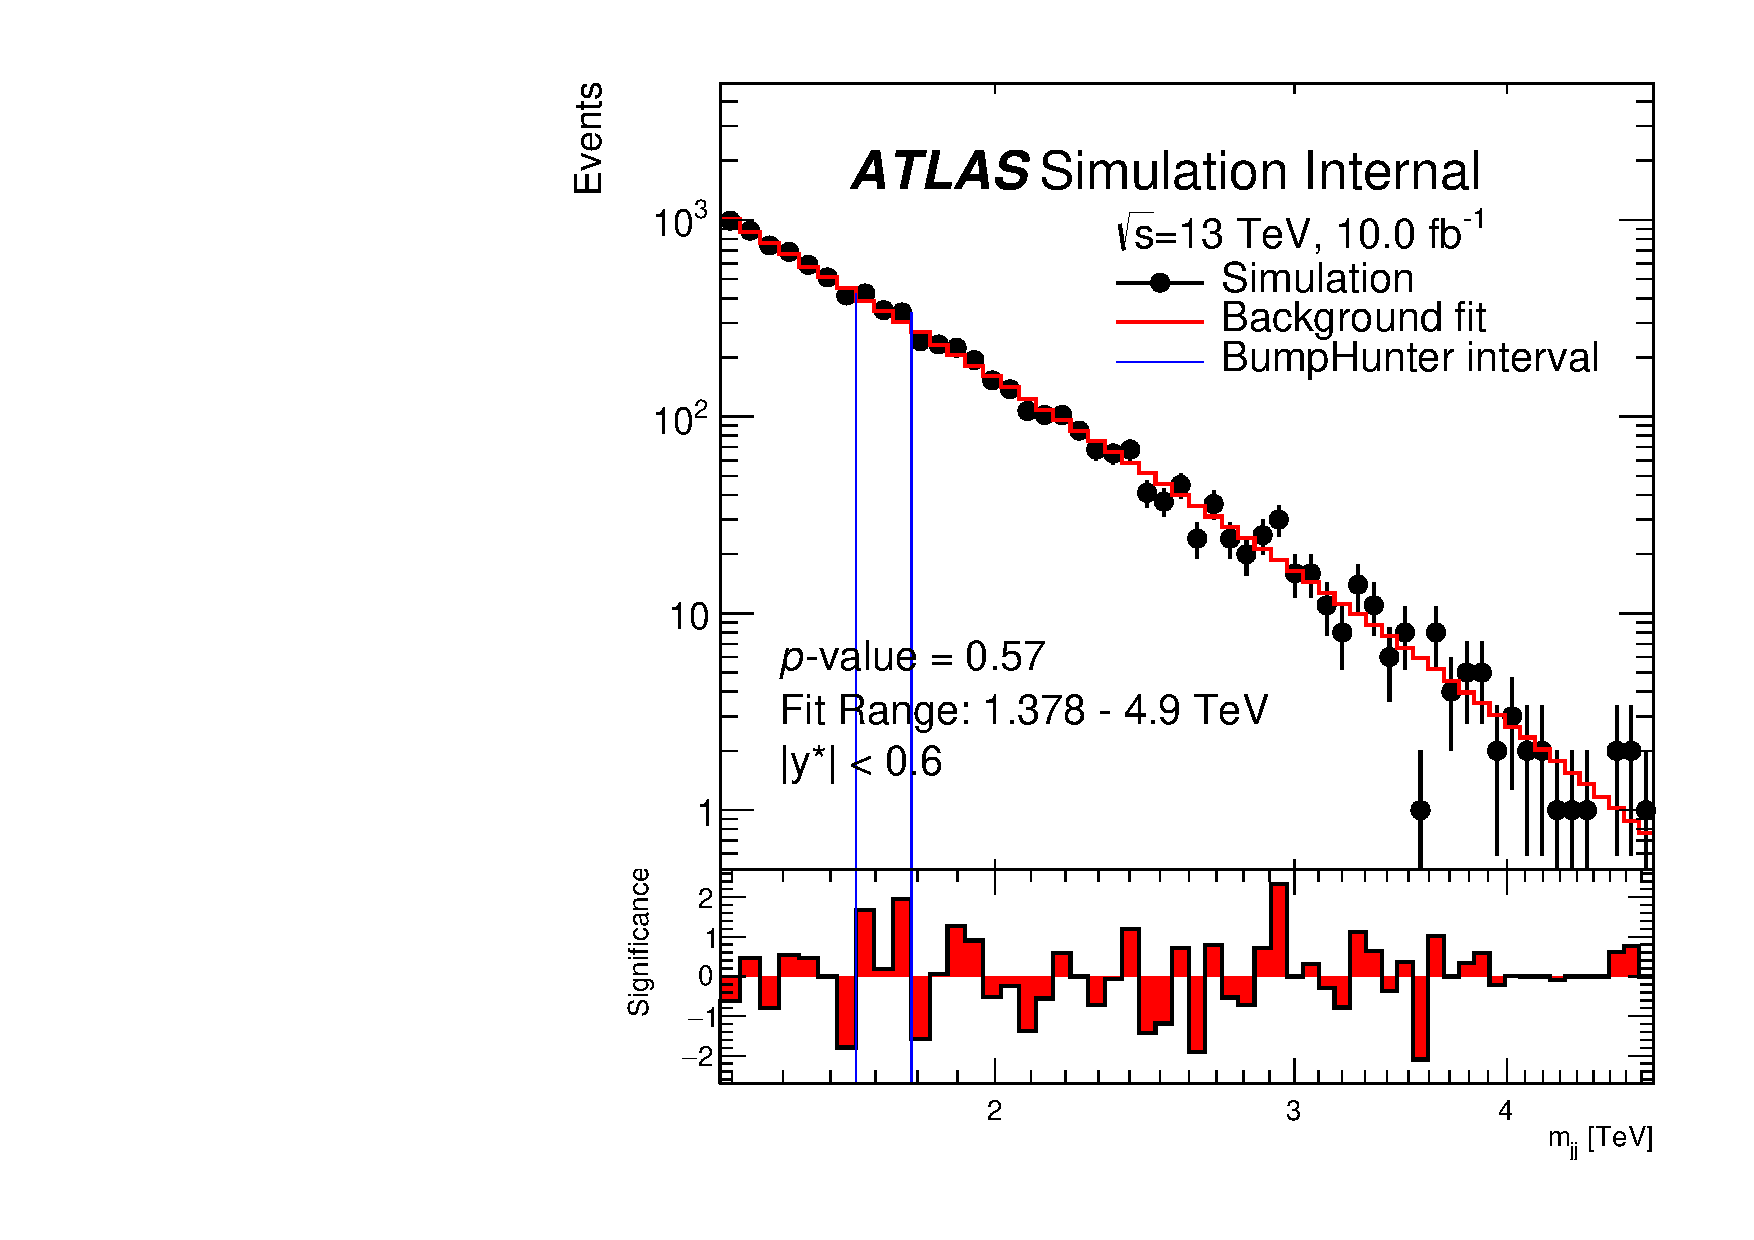
\includegraphics[width=0.47\linewidth, angle=0]{figs/Dibjet/ICHEP/SpuriousSignal/mbb_fix_8585_figure1_10fb_v10.pdf}}
    \subcaptionbox{$\geq$1 $b$-tag}{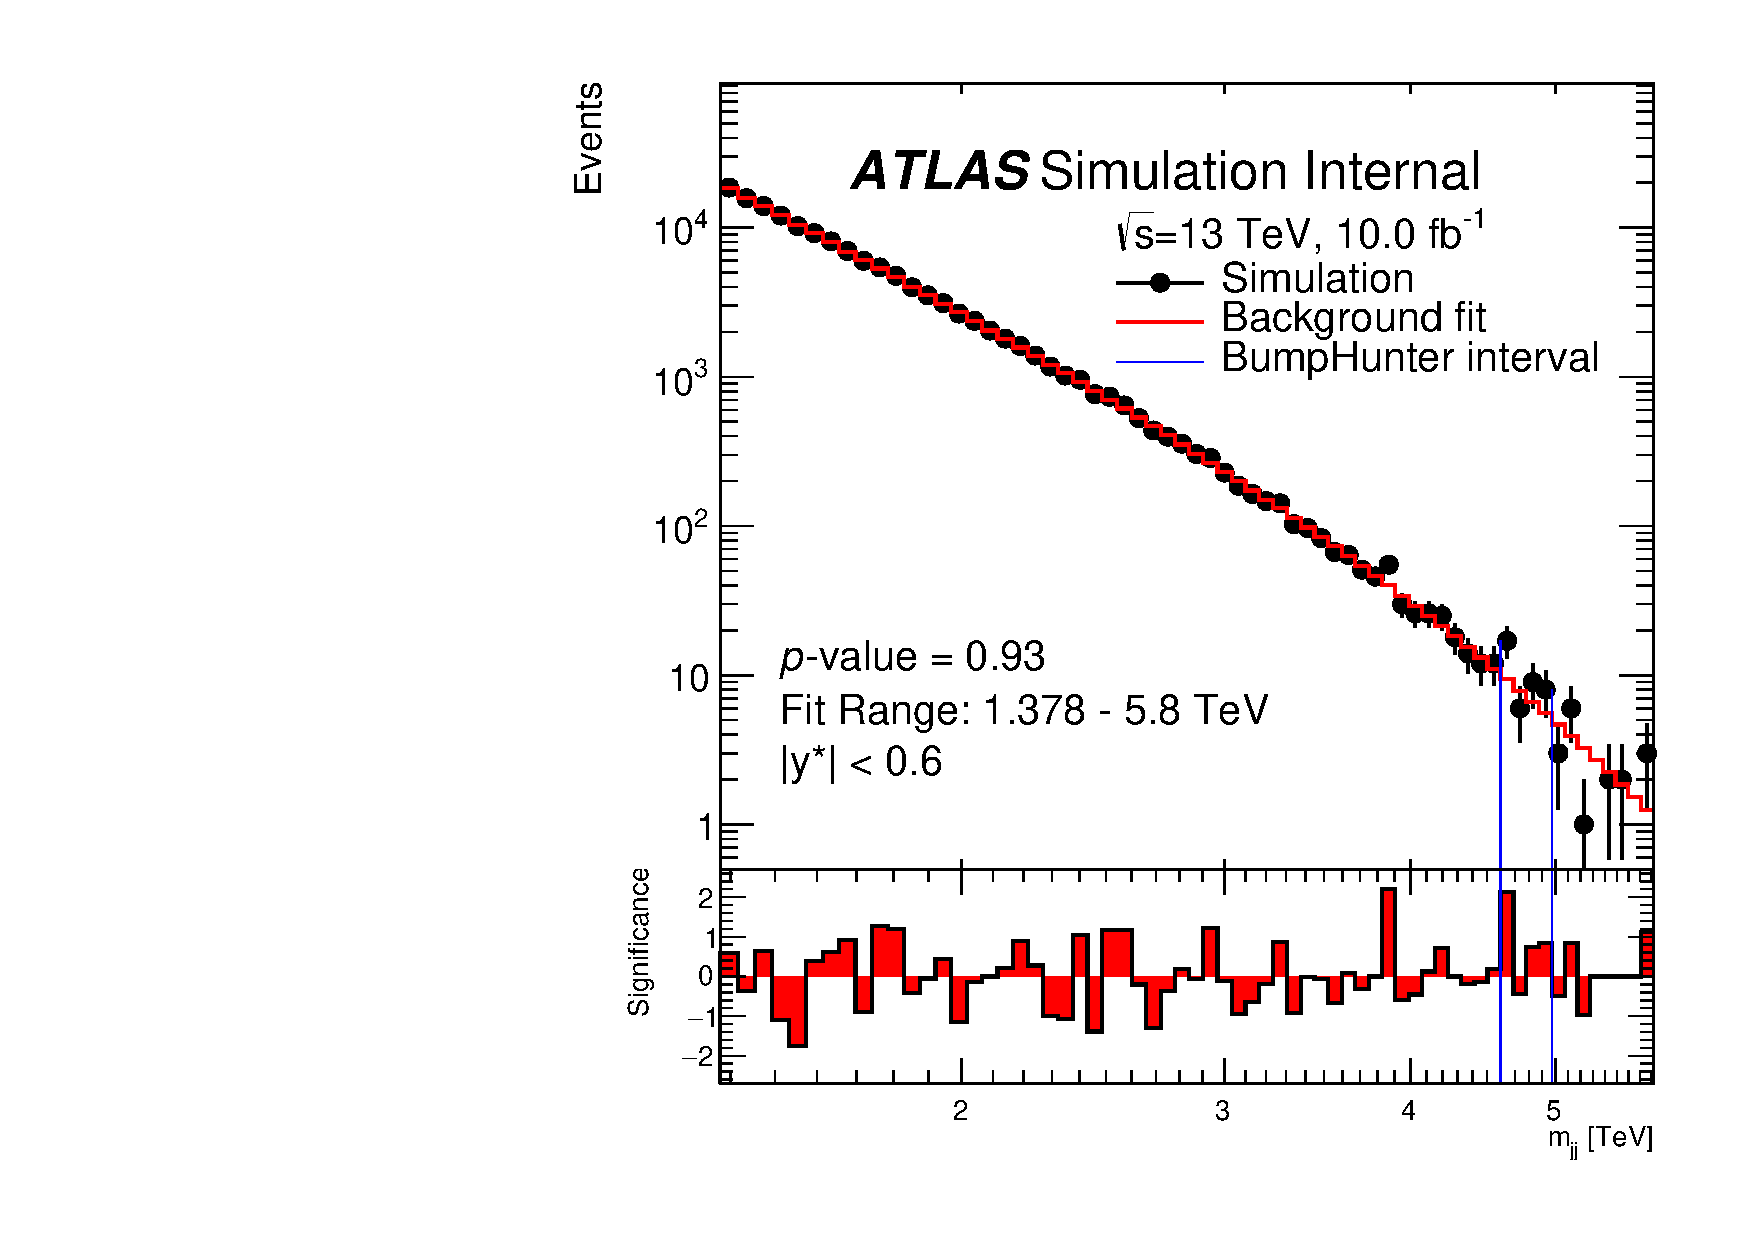
\includegraphics[width=0.47\linewidth, angle=0]{figs/Dibjet/ICHEP/SpuriousSignal/mbj_inc_fix_8585_figure1_10fb_v10.pdf}}
  \end{center}
  \caption{A data-like distribution taken from multi-jet simulation for the (a) 2 $b$-tag and (b) $\geq$1 $b$-tag,
    category, fitted to using the 3 parameter fit function.
    The BumpHunter algorithm is run to identify the most discrepant excess, as indicated by the blue lines.
    Pseudo-experiments are used to assign the excess a $p$-value, which is shown on the plot.
    The \textit{Summer16+15} dataset event selection has been applied.}
  \label{fig:DataLikeSearchPhase}
\end{figure}

\begin{figure}[!ht]
  \begin{center}
    \captionsetup[subfigure]{aboveskip=0pt,justification=centering}
    \subcaptionbox{BumpHunter}{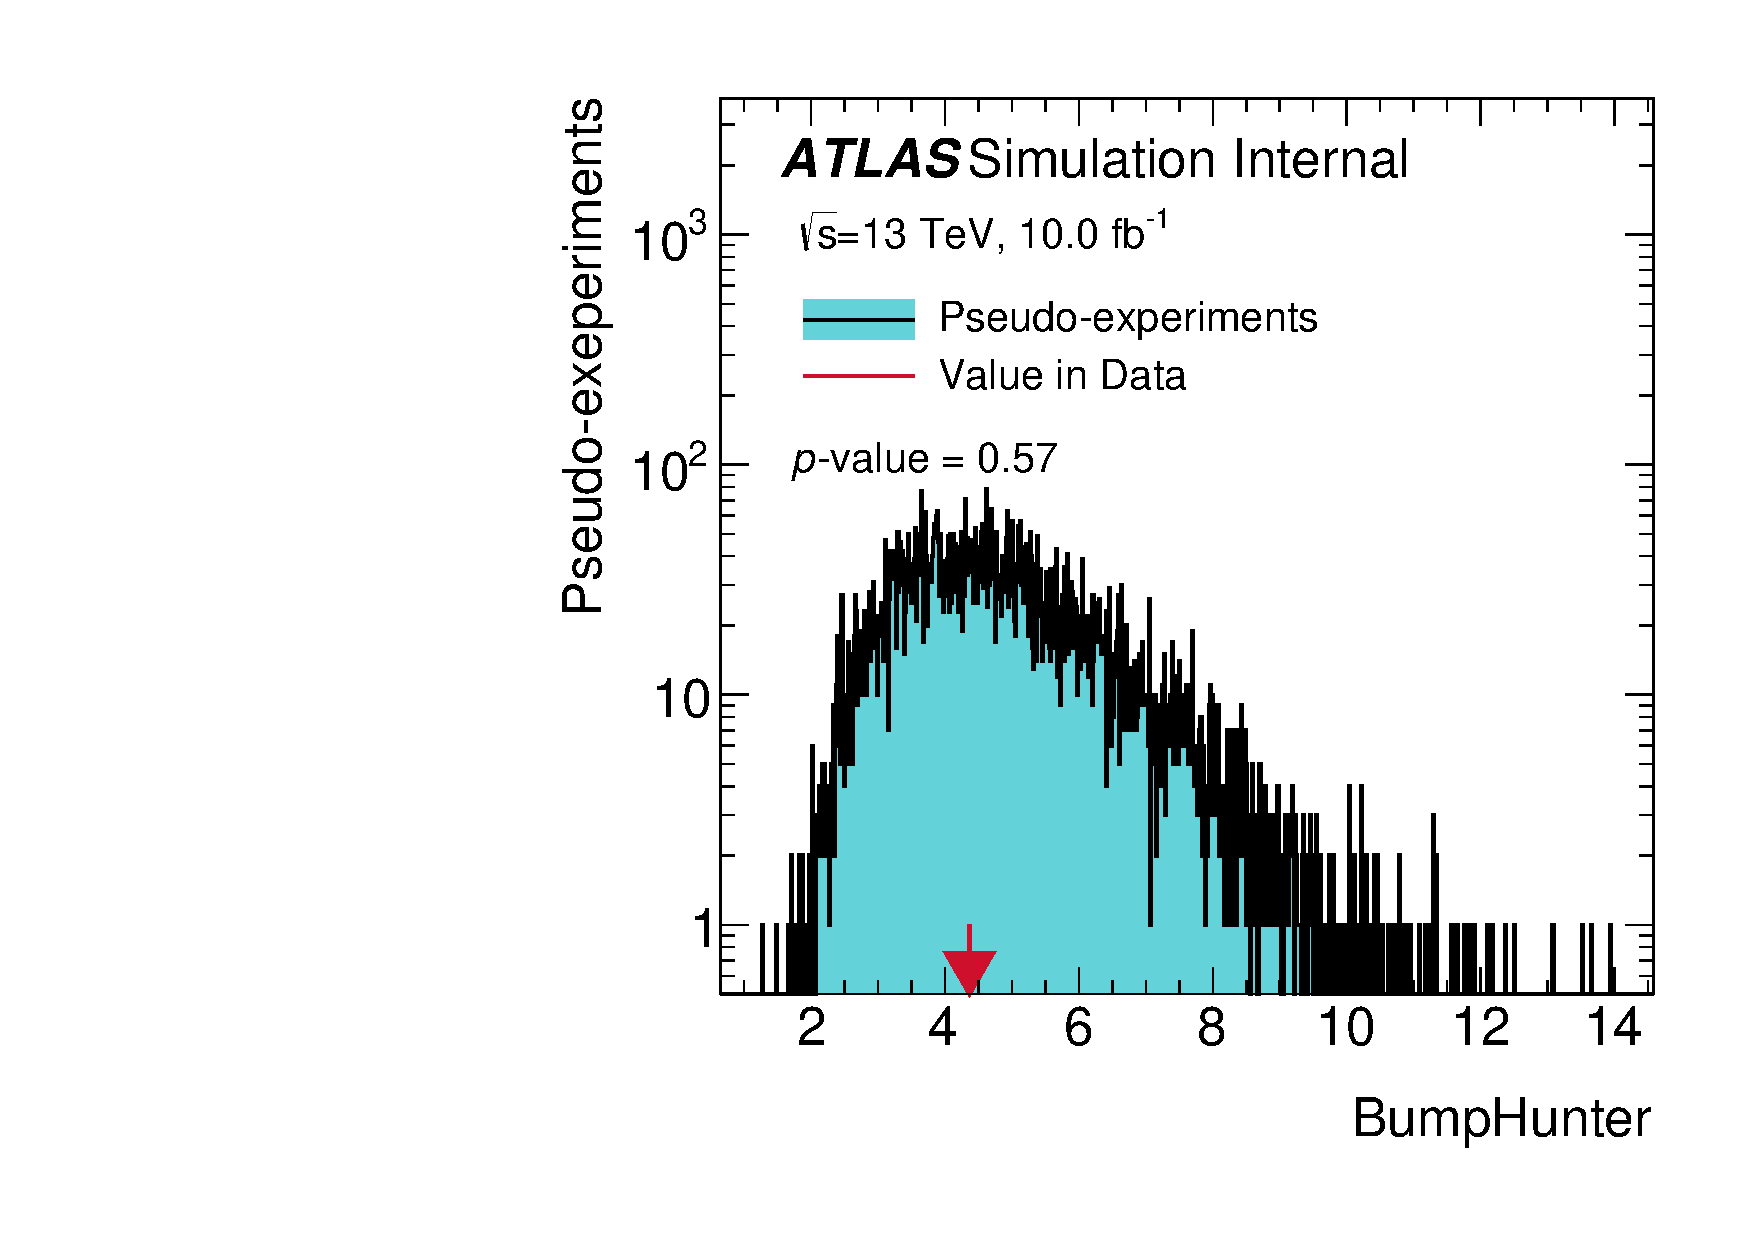
\includegraphics[width=0.47\linewidth, angle=0]{figs/Dibjet/ICHEP/SpuriousSignal/mbb_fix_8585_bumpHunterStatPlot_10fb_v10.pdf}\label{fig:DataLikeBumpHunterStatPlot_bb}}
    \subcaptionbox{BumpHunter}{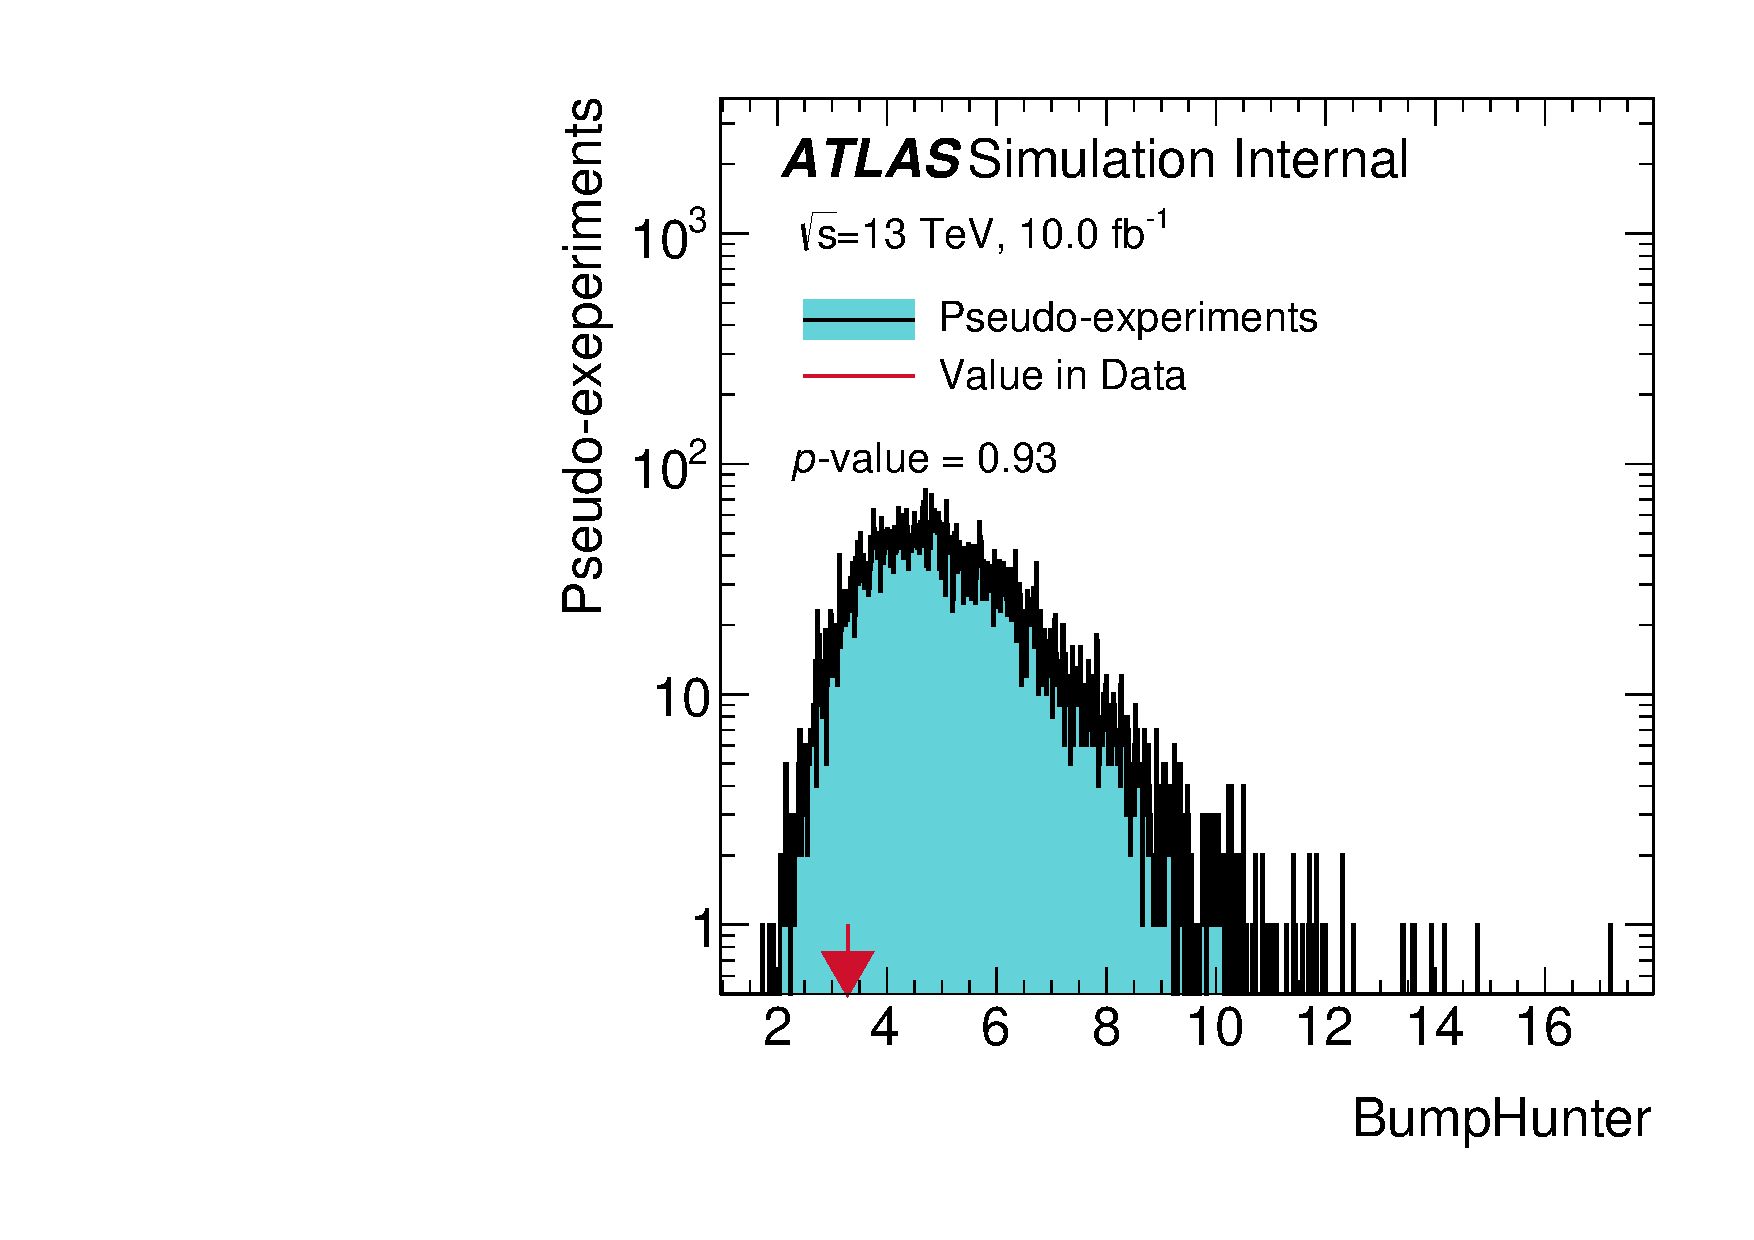
\includegraphics[width=0.47\linewidth, angle=0]{figs/Dibjet/ICHEP/SpuriousSignal/mbj_inc_fix_8585_bumpHunterStatPlot_10fb_v10.pdf}\label{fig:DataLikeBumpHunterStatPlot_bj}}
  \end{center}
  \caption{The distribution of the BumpHunter test statistic for 10,000 pseudo experiments compared
    to the value observed in a data-like distribution from the (a) 2 $b$-tag category and (b) $\geq$1 $b$-tag category.
    The fraction of pseudo-experiments with a BumpHunter test statistic greater than the value in data is the estimation of the respective $p$-value.}
  \label{fig:DataLikeStatPlots_bh}
\end{figure}


%\begin{figure}[!ht]
%  \begin{center}
%   \captionsetup[subfigure]{aboveskip=0pt,justification=centering}
%  \subcaptionbox{BumpHunter}{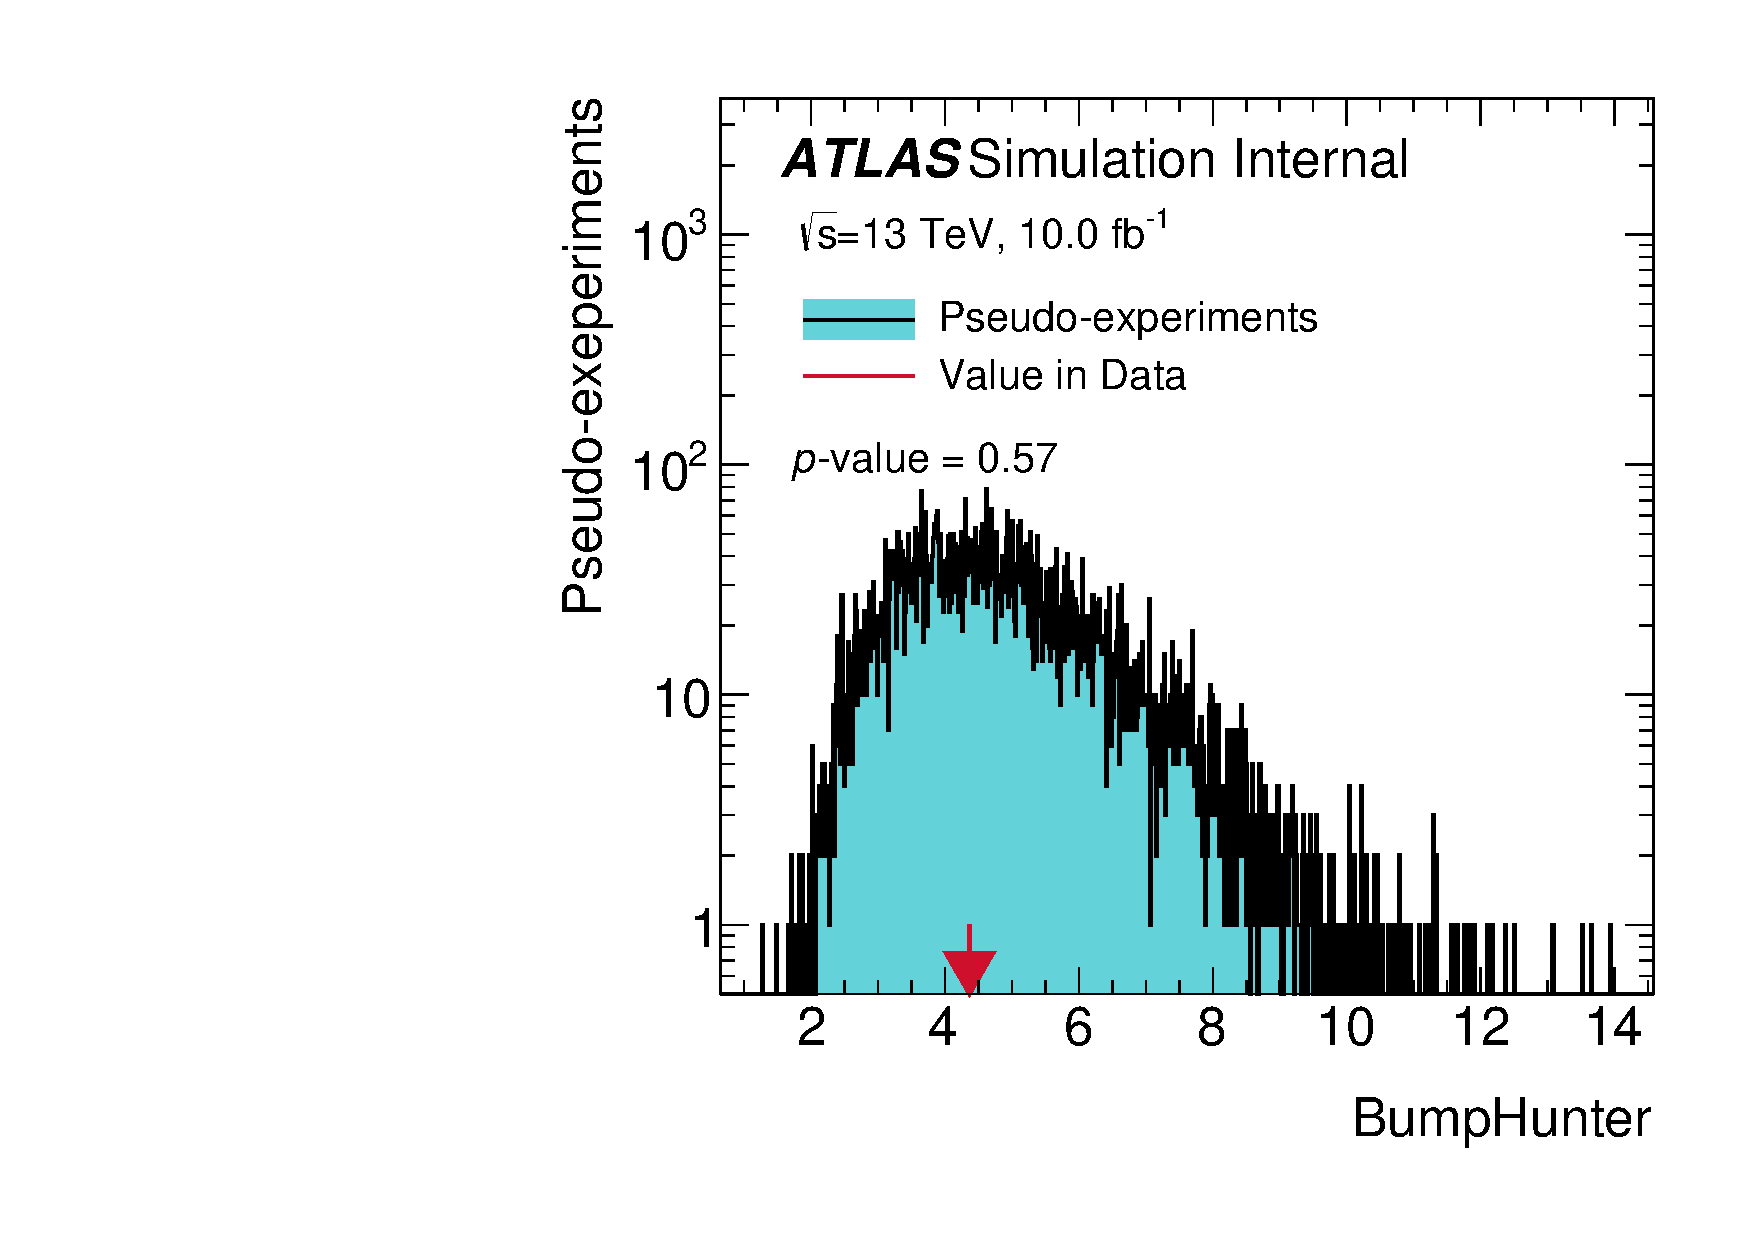
\includegraphics[width=0.47\linewidth, angle=0]{figs/Dibjet/ICHEP/SpuriousSignal/mbb_fix_8585_bumpHunterStatPlot_10fb_v10.pdf}\label{fig:DataLikeBumpHunterStatPlot_bb}}
%  \subcaptionbox{DeficitHunter}{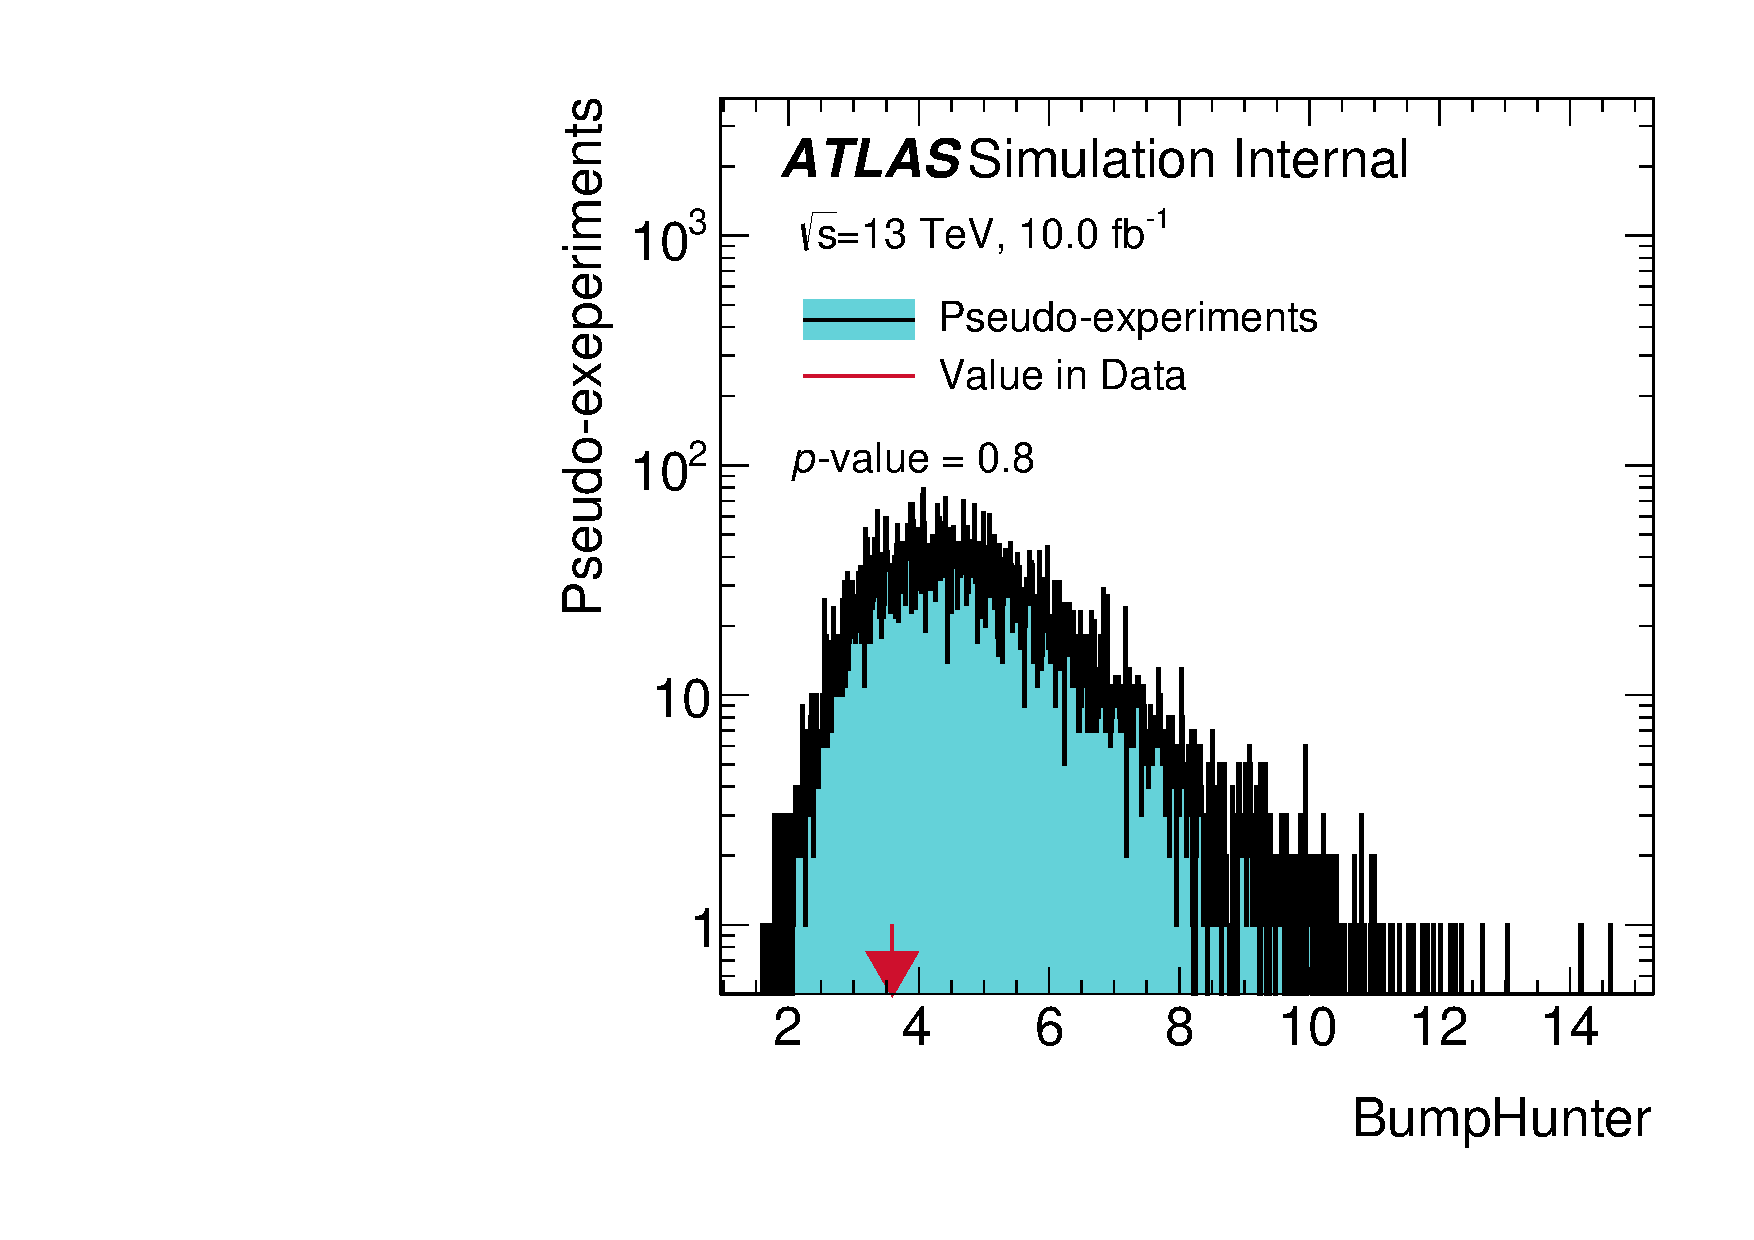
\includegraphics[width=0.47\linewidth, angle=0]{figs/Dibjet/ICHEP/SpuriousSignal/mbb_fix_8585_deficitOnlyHunterStatPlot_10fb_v10.pdf}\label{fig:DataLikeDeficitOnlyHunterStatPlot_bb}}  
%  \subcaptionbox{$\chi^{2}$}{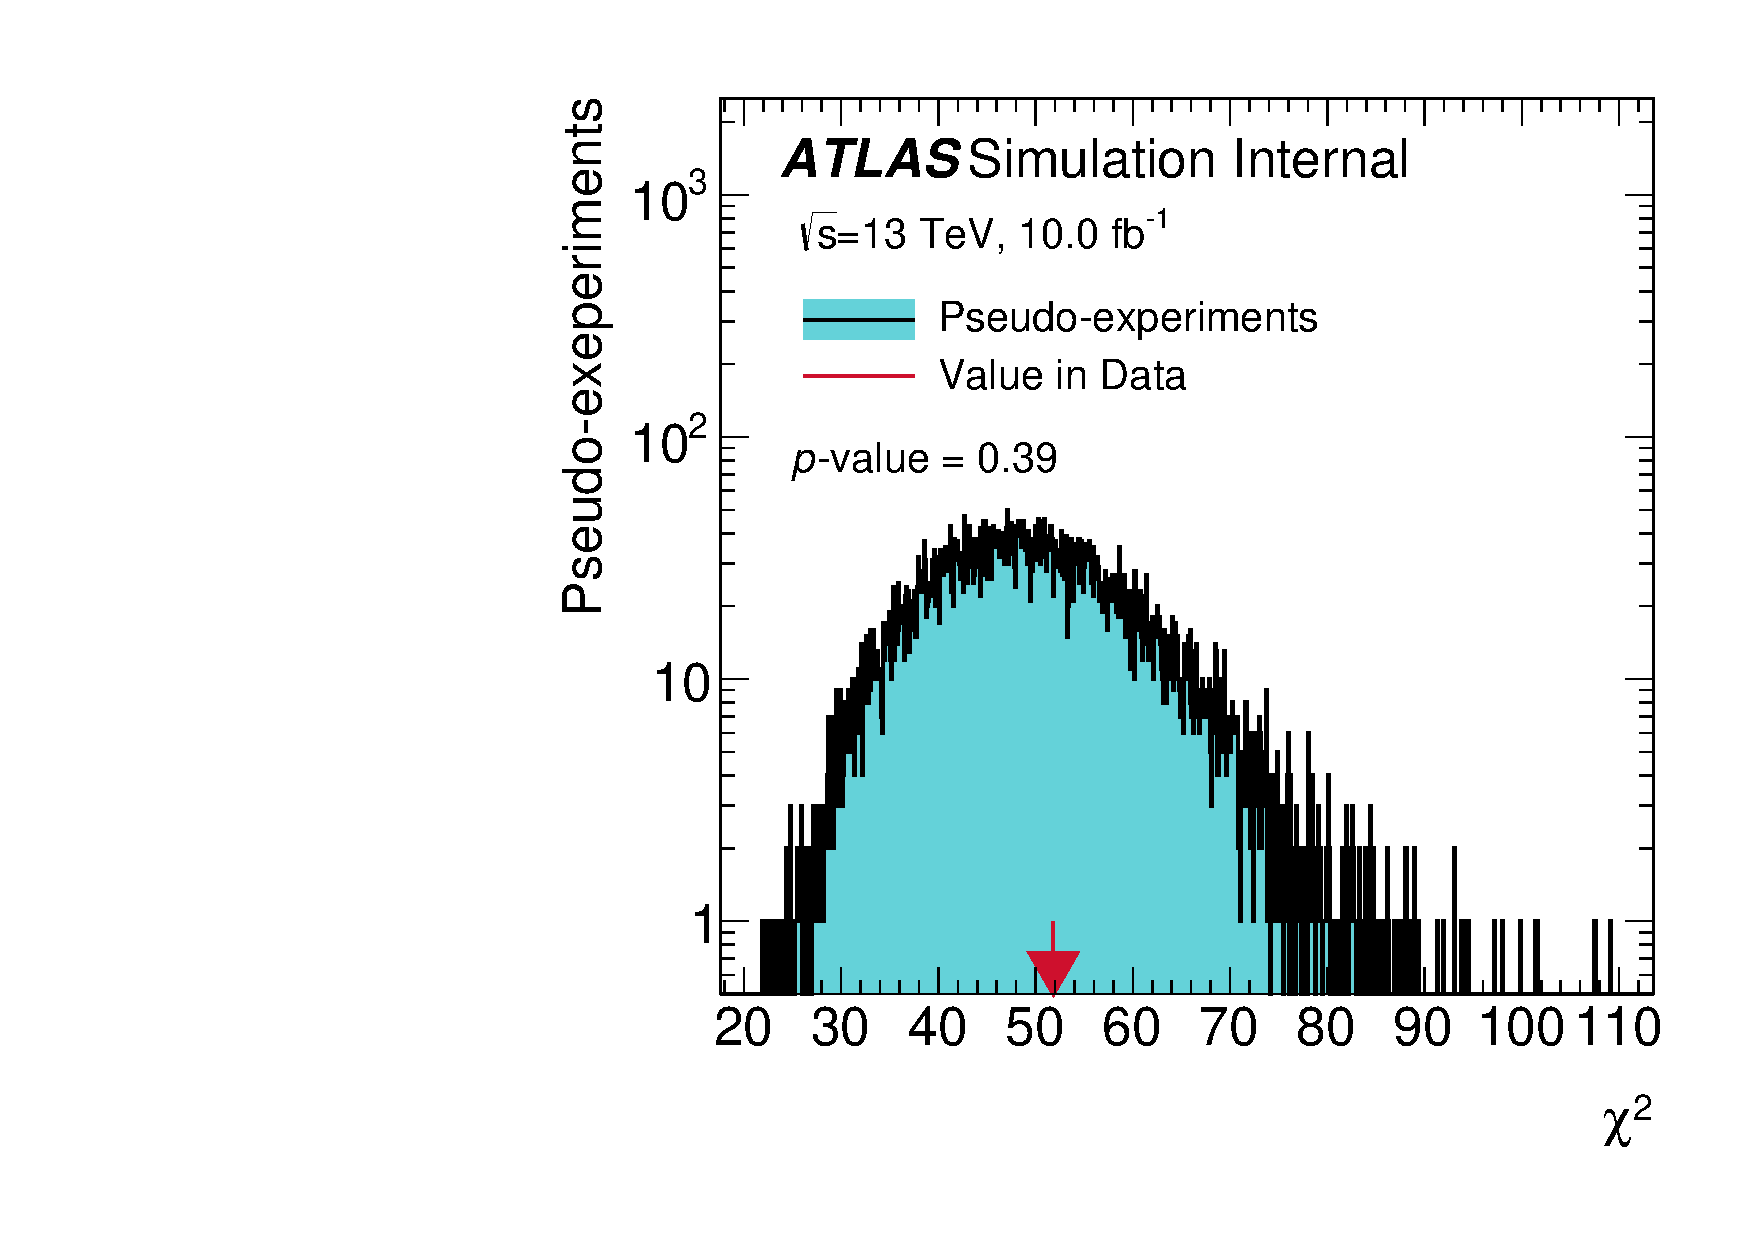
\includegraphics[width=0.47\linewidth, angle=0]{figs/Dibjet/ICHEP/SpuriousSignal/mbb_fix_8585_chi2StatPlot_10fb_v10.pdf}\label{fig:DataLikeChi2StatPlot_bb}}  
%  \end{center}
%  \caption{The distribution of the (a) BumpHunter test statistic, (b) DeficitHunter test statistic and (c) $\chi^{2}$ test statistic for 10,000 pseudo experiments
%    compared to the value found in a data-like distribution for the 2 $b$-tag category. 
%    The fraction of pseudo-experiments with a BumpHunter, DeficitHunter or $\chi^{2}$ test statistic greater than the value in data is the estimation of the respective $p$-value.}
%  \label{fig:DataLikeStatPlots_bb}
%  \begin{center}
%   \captionsetup[subfigure]{aboveskip=0pt,justification=centering}
%  \subcaptionbox{BumpHunter}{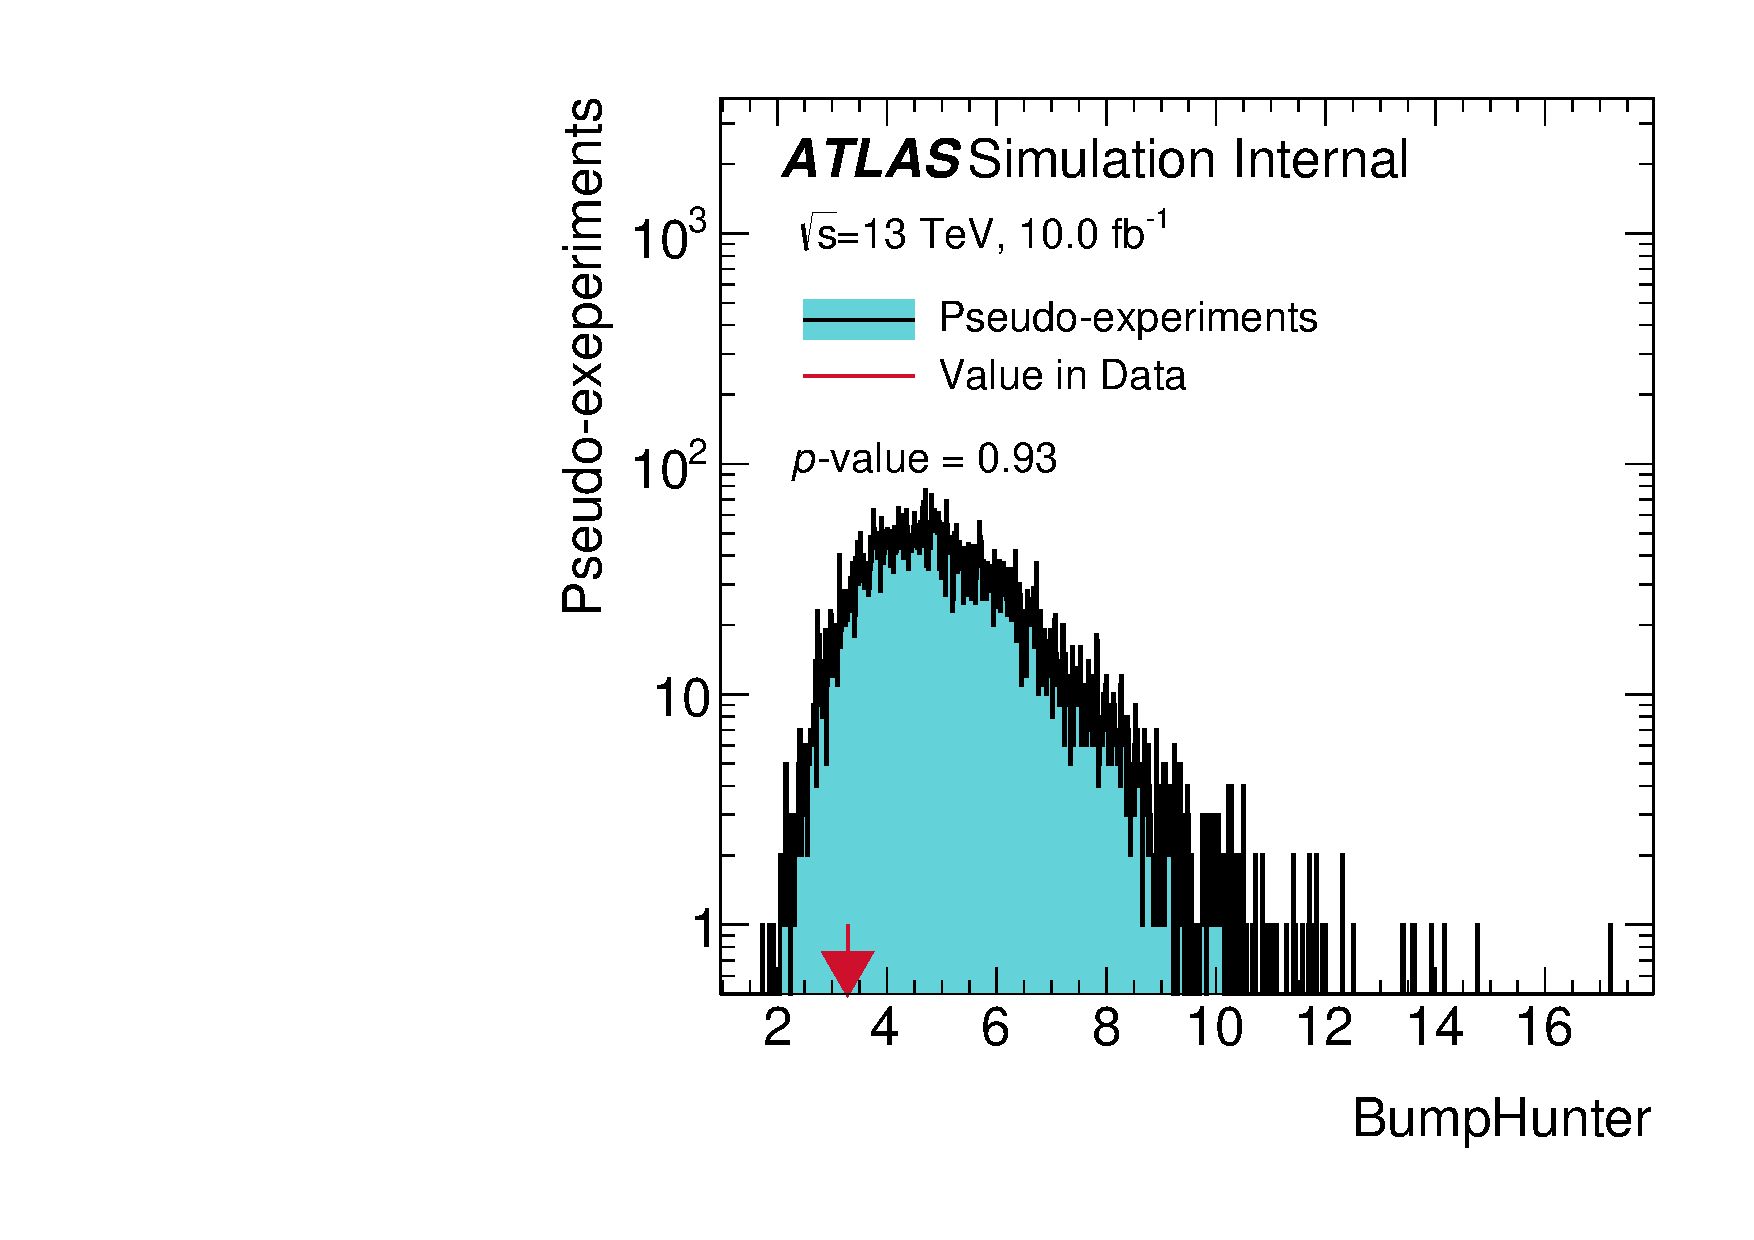
\includegraphics[width=0.47\linewidth, angle=0]{figs/Dibjet/ICHEP/SpuriousSignal/mbj_inc_fix_8585_bumpHunterStatPlot_10fb_v10.pdf}\label{fig:DataLikeBumpHunterStatPlot_bj}}
%  \subcaptionbox{DeficitHunter}{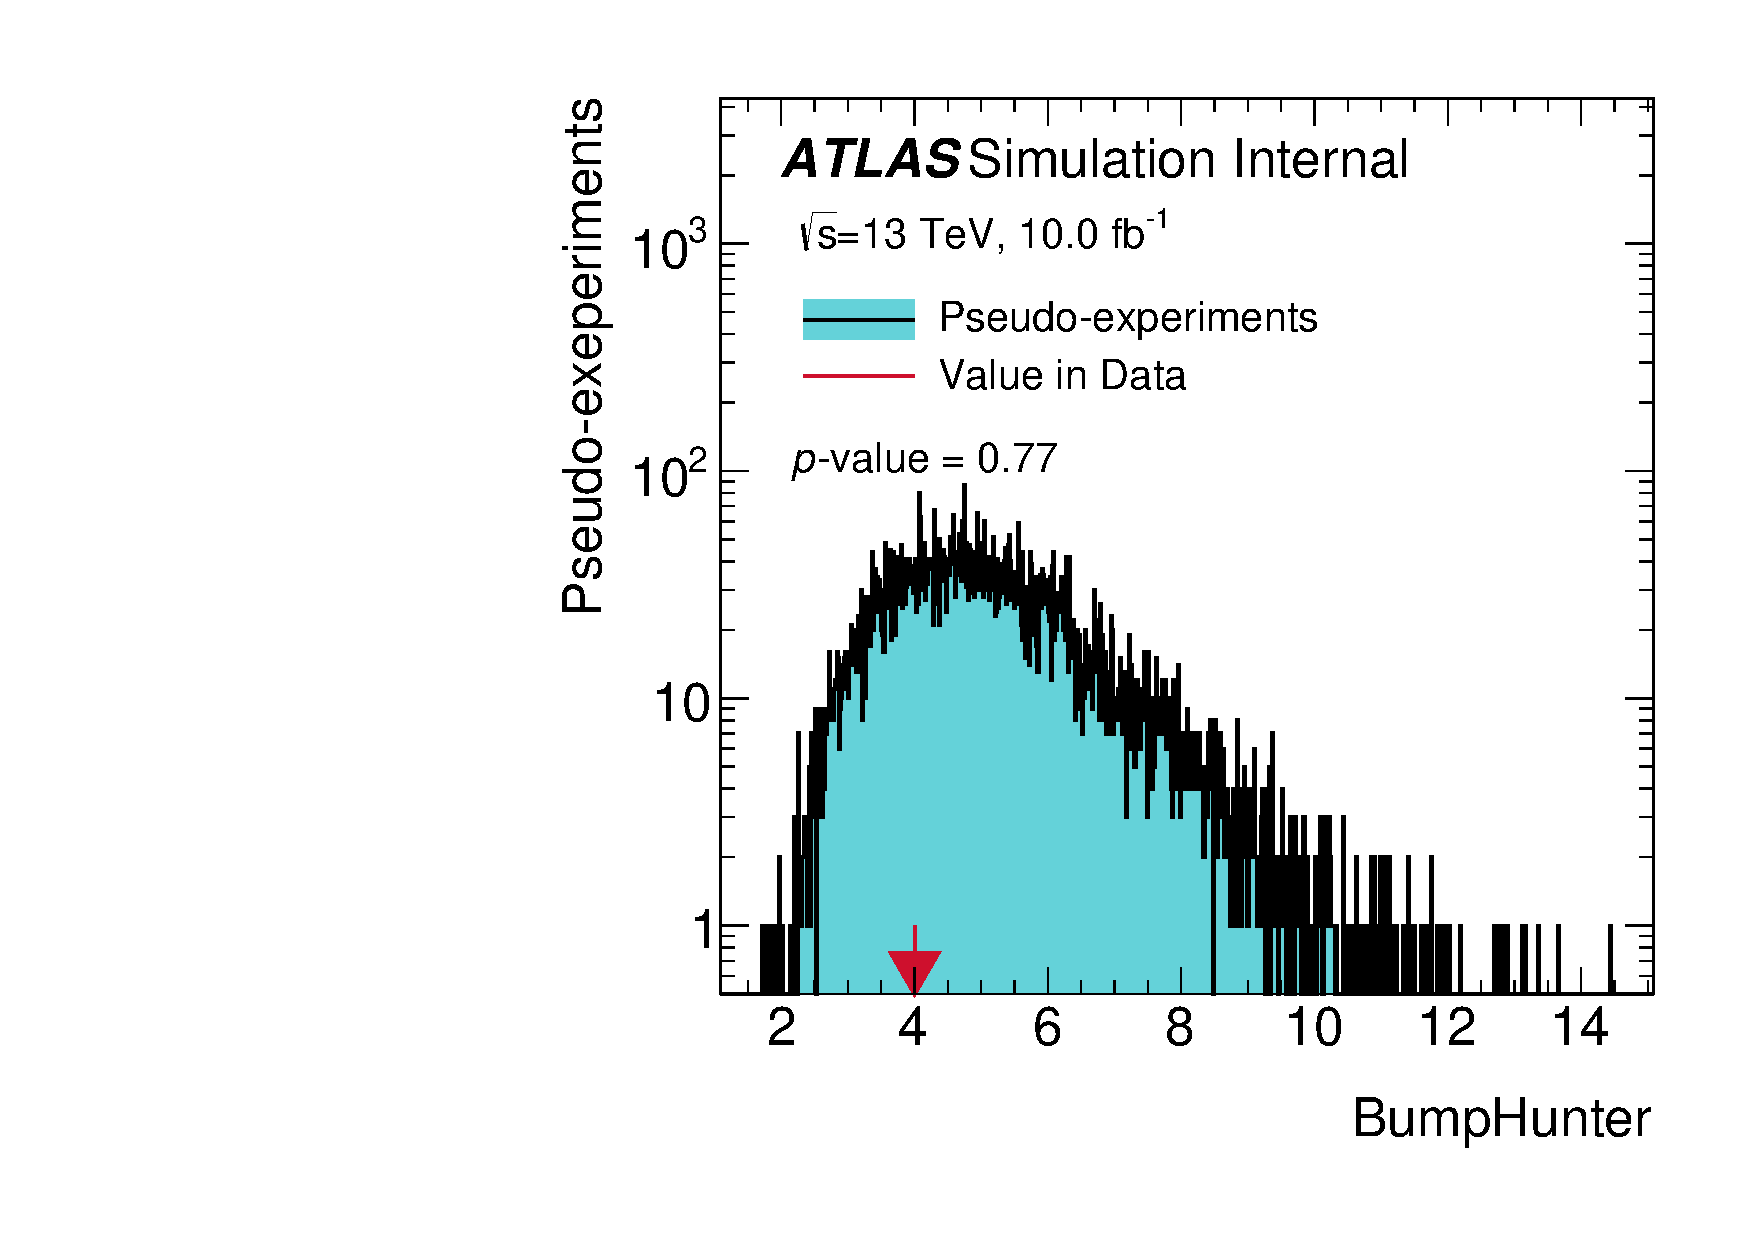
\includegraphics[width=0.47\linewidth, angle=0]{figs/Dibjet/ICHEP/SpuriousSignal/mbj_inc_fix_8585_deficitOnlyHunterStatPlot_10fb_v10.pdf}\label{fig:DataLikeDeficitOnlyHunterStatPlot_bj}}  
%  \subcaptionbox{$\chi^{2}$}{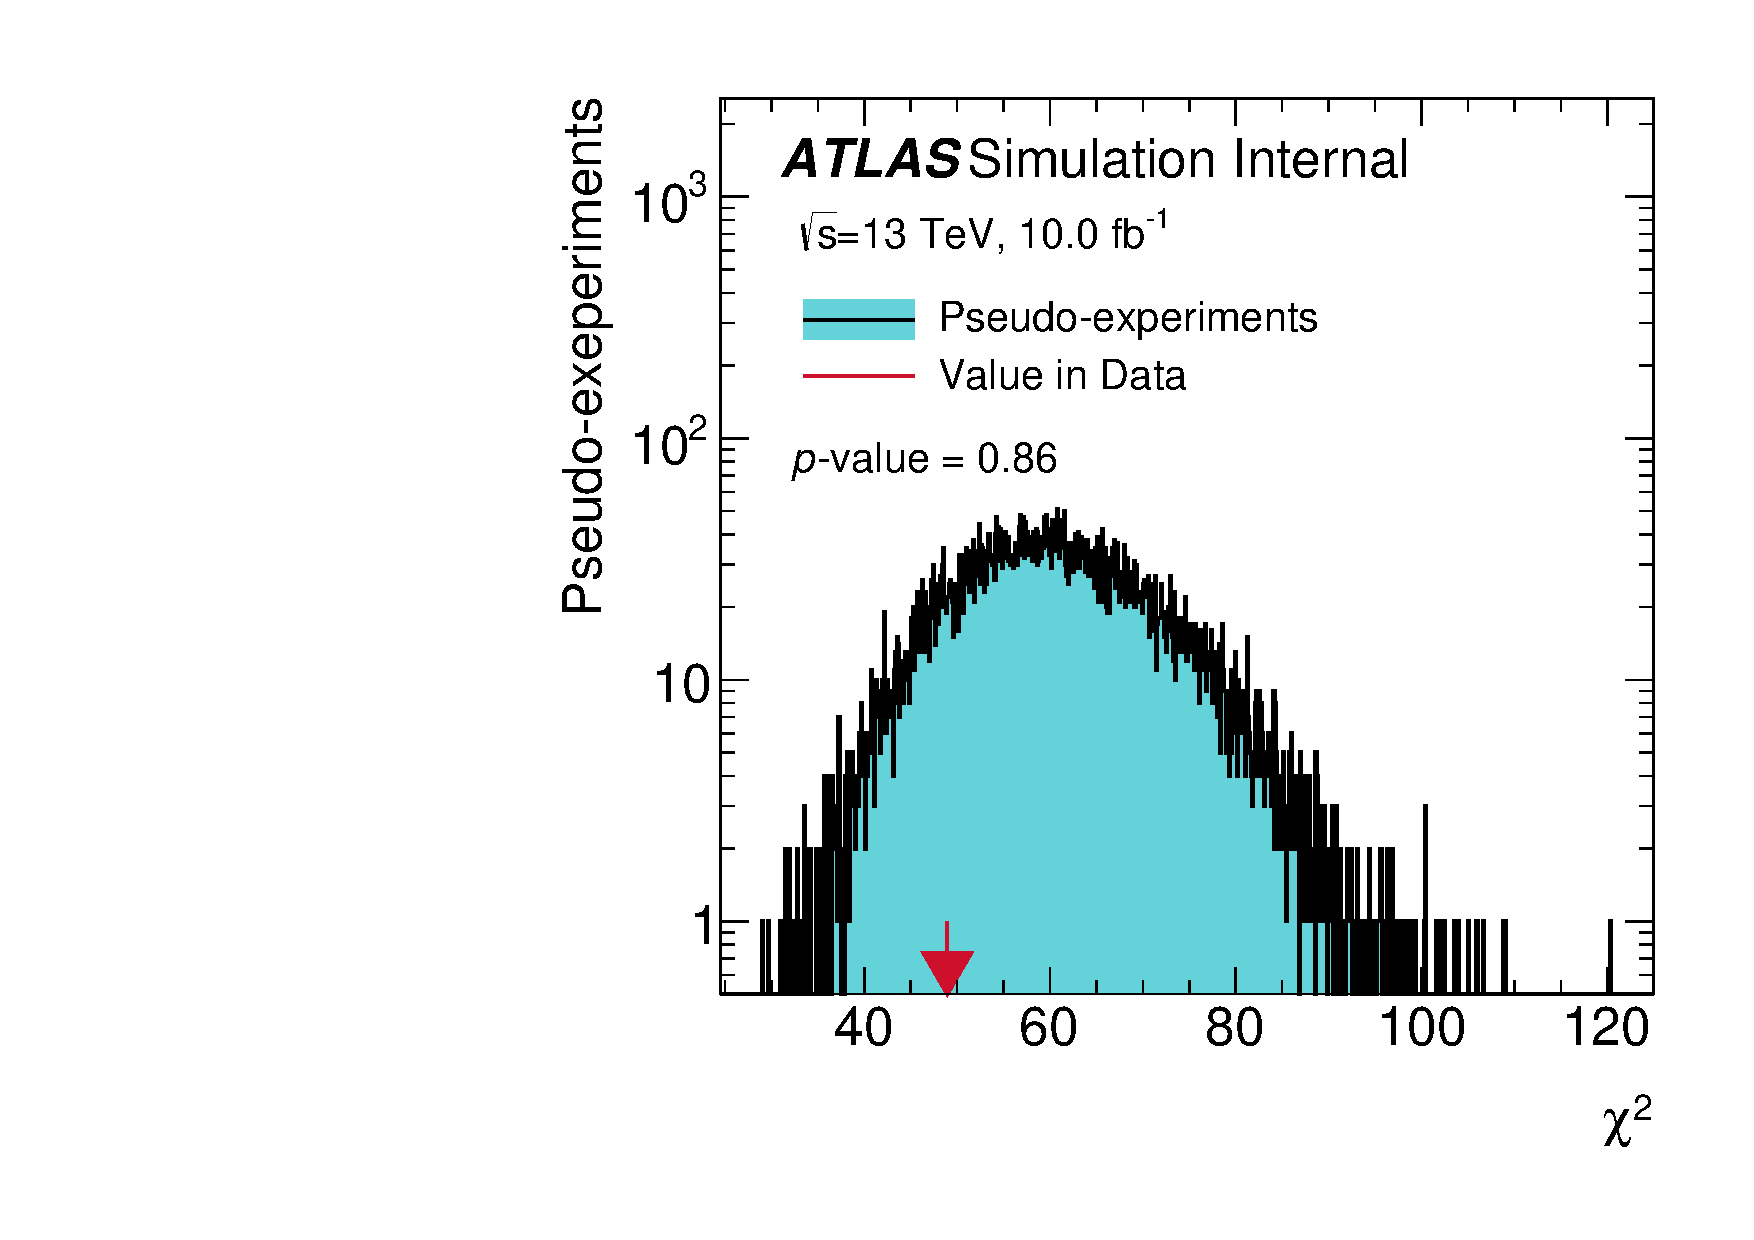
\includegraphics[width=0.47\linewidth, angle=0]{figs/Dibjet/ICHEP/SpuriousSignal/mbj_inc_fix_8585_chi2StatPlot_10fb_v10.pdf}\label{fig:DataLikeChi2StatPlot_bj}}  
%  \end{center}
%  \caption{The distribution of the (a) BumpHunter test statistic, (b) DeficitHunter test statistic and (c) $\chi^{2}$ test statistic for 10,000 pseudo experiments
%    compared to the value found in a data-like distribution for the $\geq$1 $b$-tag category.
%  The fraction of pseudo-experiments with a BumpHunter, DeficitHunter or $\chi^{2}$ test statistic greater than the value in data is the estimation of the respective $p$-value. }
%  \label{fig:DataLikeStatPlots_bj}
%\end{figure}


Many different Poisson fluctuations can be applied to the scaled distribution to give many different data-like distributions that can be fitted,
and each fit will give a different BumpHunter and $\chi^{2}$ $p$-value.
Figure~\ref{fig:pValueHists_bb} and Figure~\ref{fig:pValueHists_bj} shows the distribution of BumpHunter, DeficitHunter and $\chi^{2}$ $p$-values for 200 different data-like distributions,
for the 2 $b$-tag and $\geq$1 $b$-tag category.
There is no evidence of a fit-bias causing spurious signal in either category,
which could be seen by a bias towards low BumpHunter $p$-values causing fake signals
or a bias toward low DeficitHunter $p$-values causing fake deficits.
The distribution of the $\chi^{2}$ $p$-values also indicates that there is good fit quality in both tagging categories.

Hence, it can be concluded that the 3 parameter fit function is a good description of the simulated QCD background
and that there is no evidence that spurious signal can occur.
Similar tests were performed for the 4 parameter fit function but are not presented here because,
as shown in Section~\ref{sec:bkg-summer_global},
the 3 parameter function is chosen in both categories for this data-set.

\begin{figure}[!htb]
  \begin{center}
   \captionsetup[subfigure]{aboveskip=0pt,justification=centering}
  \subcaptionbox{BumpHunter}{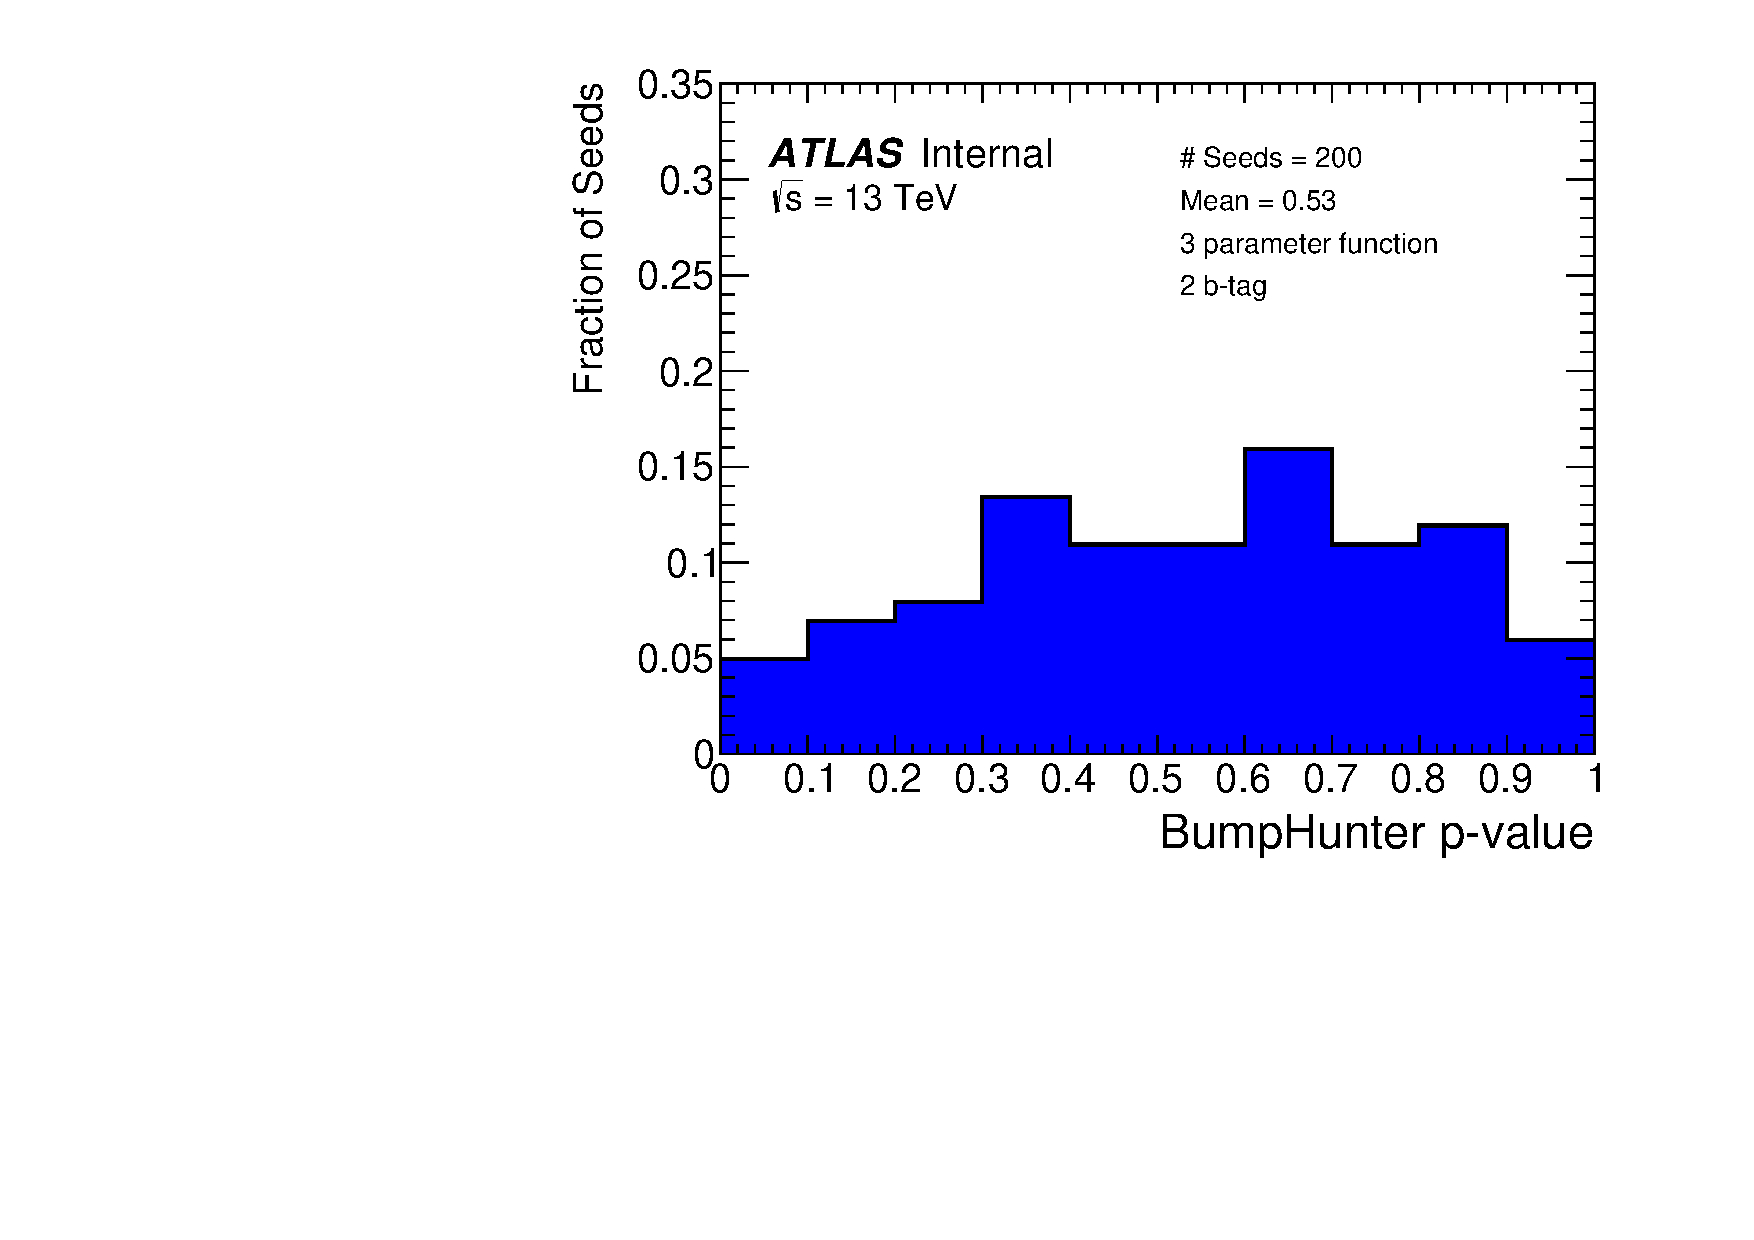
\includegraphics[width=0.32\linewidth, angle=0]{figs/Dibjet/ICHEP/SpuriousSignal/mbb_fix_8585_pValHist_bumpHunter.pdf}}
  \subcaptionbox{DeficitHunter}{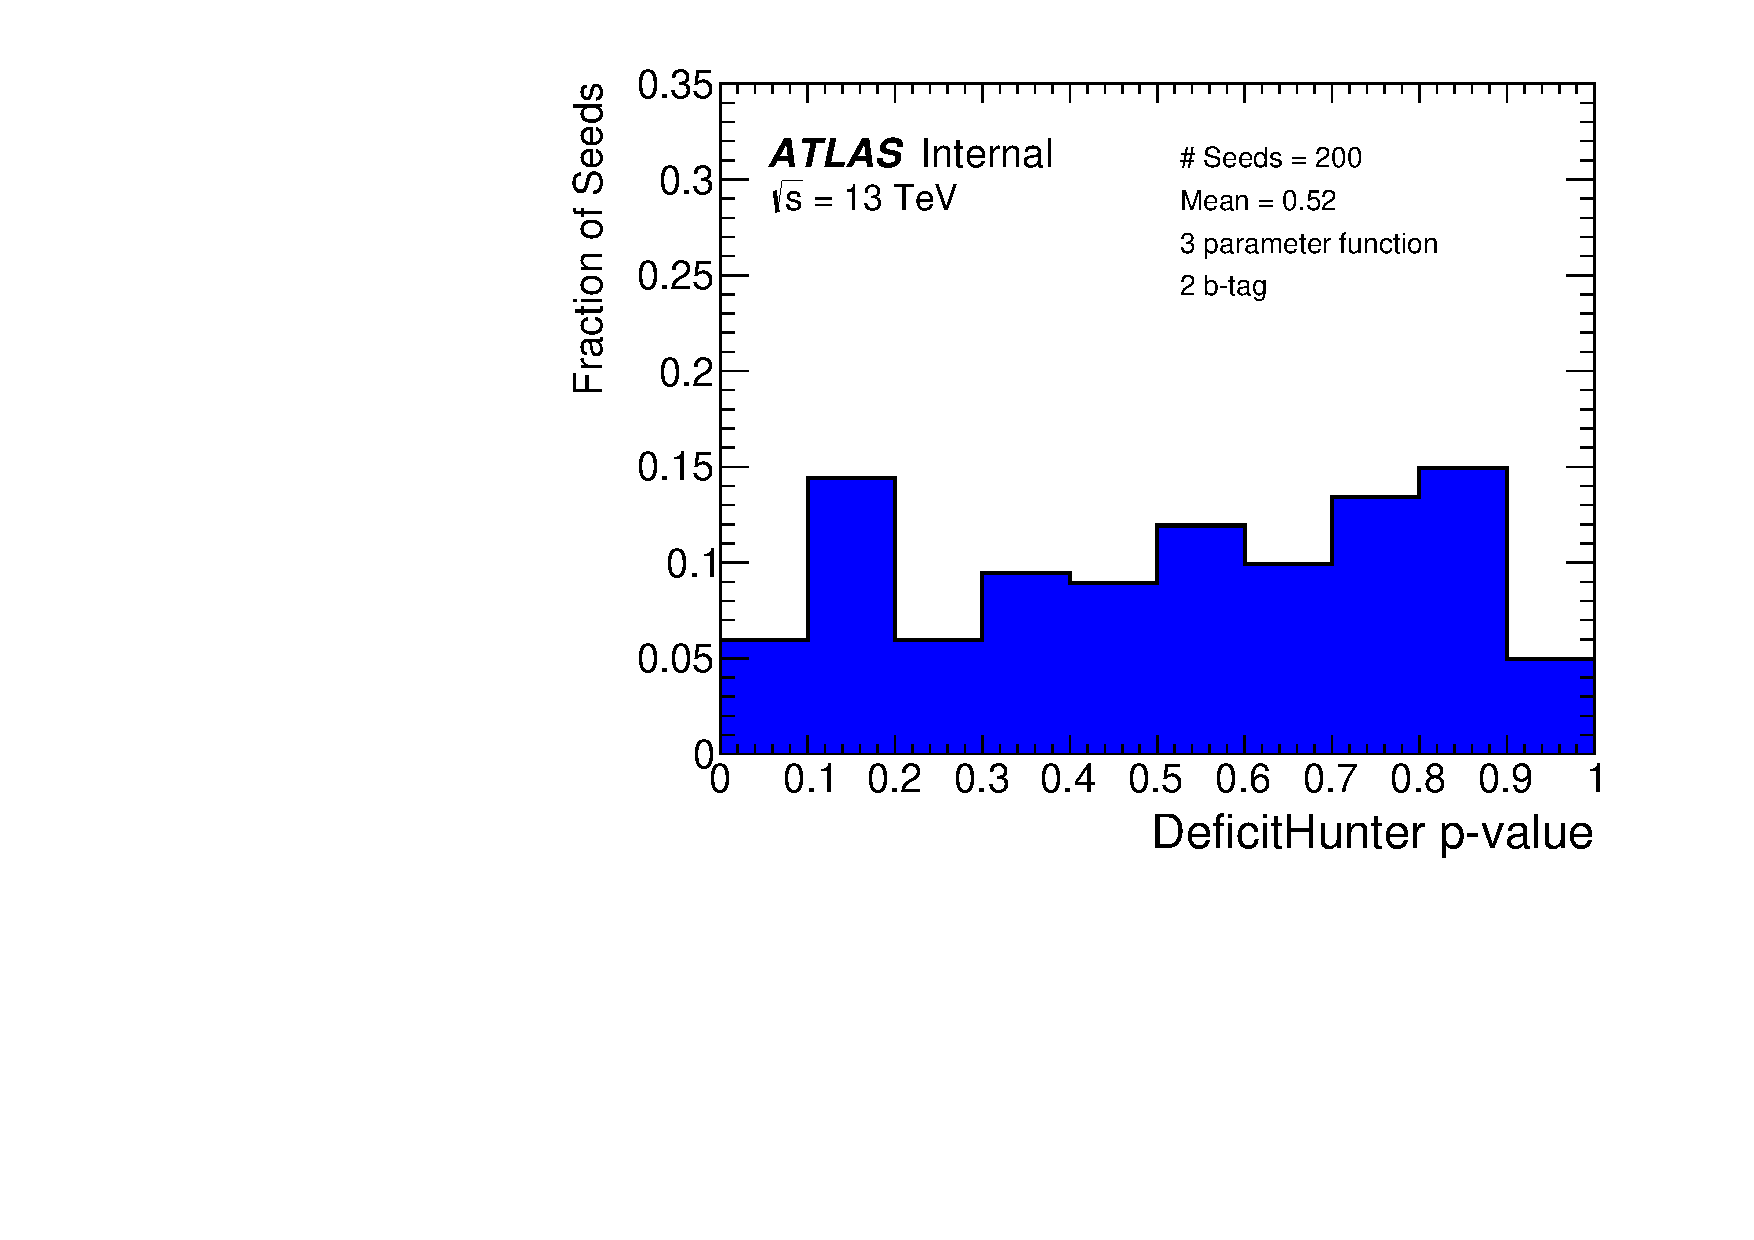
\includegraphics[width=0.32\linewidth, angle=0]{figs/Dibjet/ICHEP/SpuriousSignal/mbb_fix_8585_pValHist_deficitHunter.pdf}}
  \subcaptionbox{$\chi^{2}$}{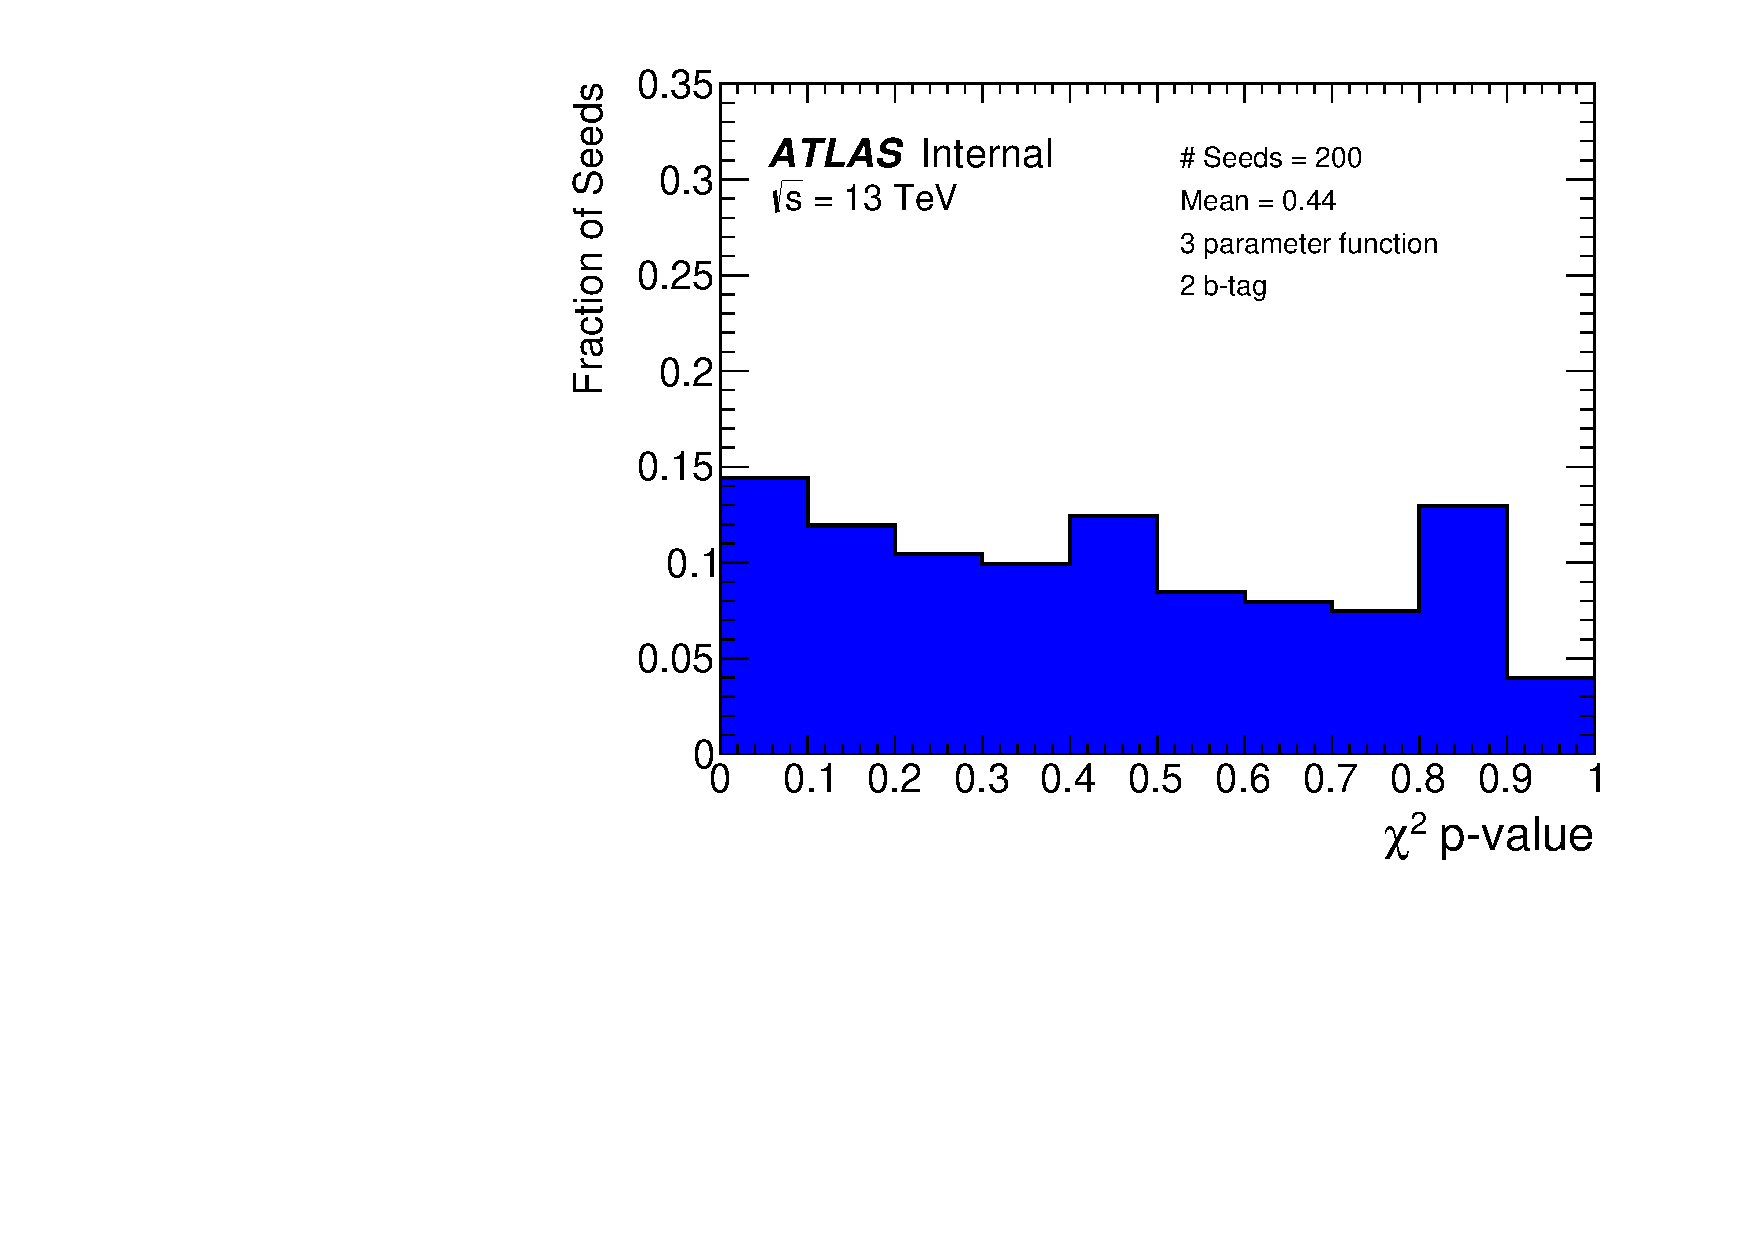
\includegraphics[width=0.32\linewidth, angle=0]{figs/Dibjet/ICHEP/SpuriousSignal/mbb_fix_8585_pValHist_chi2.pdf}}
  \end{center}
  \caption{The distribution of (a) BumpHunter, (b) DeficitHunter and (c) $\chi^{2}$ $p$-values for fits to
    200 data-like invariant mass spectra in the 2 $b$-tag category.
    The \textit{Summer16+15} dataset event selection has been applied.}
  \label{fig:pValueHists_bb}
\end{figure}   
\begin{figure}[!htb]
  \begin{center}
   \captionsetup[subfigure]{aboveskip=0pt,justification=centering}
  \subcaptionbox{BumpHunter}{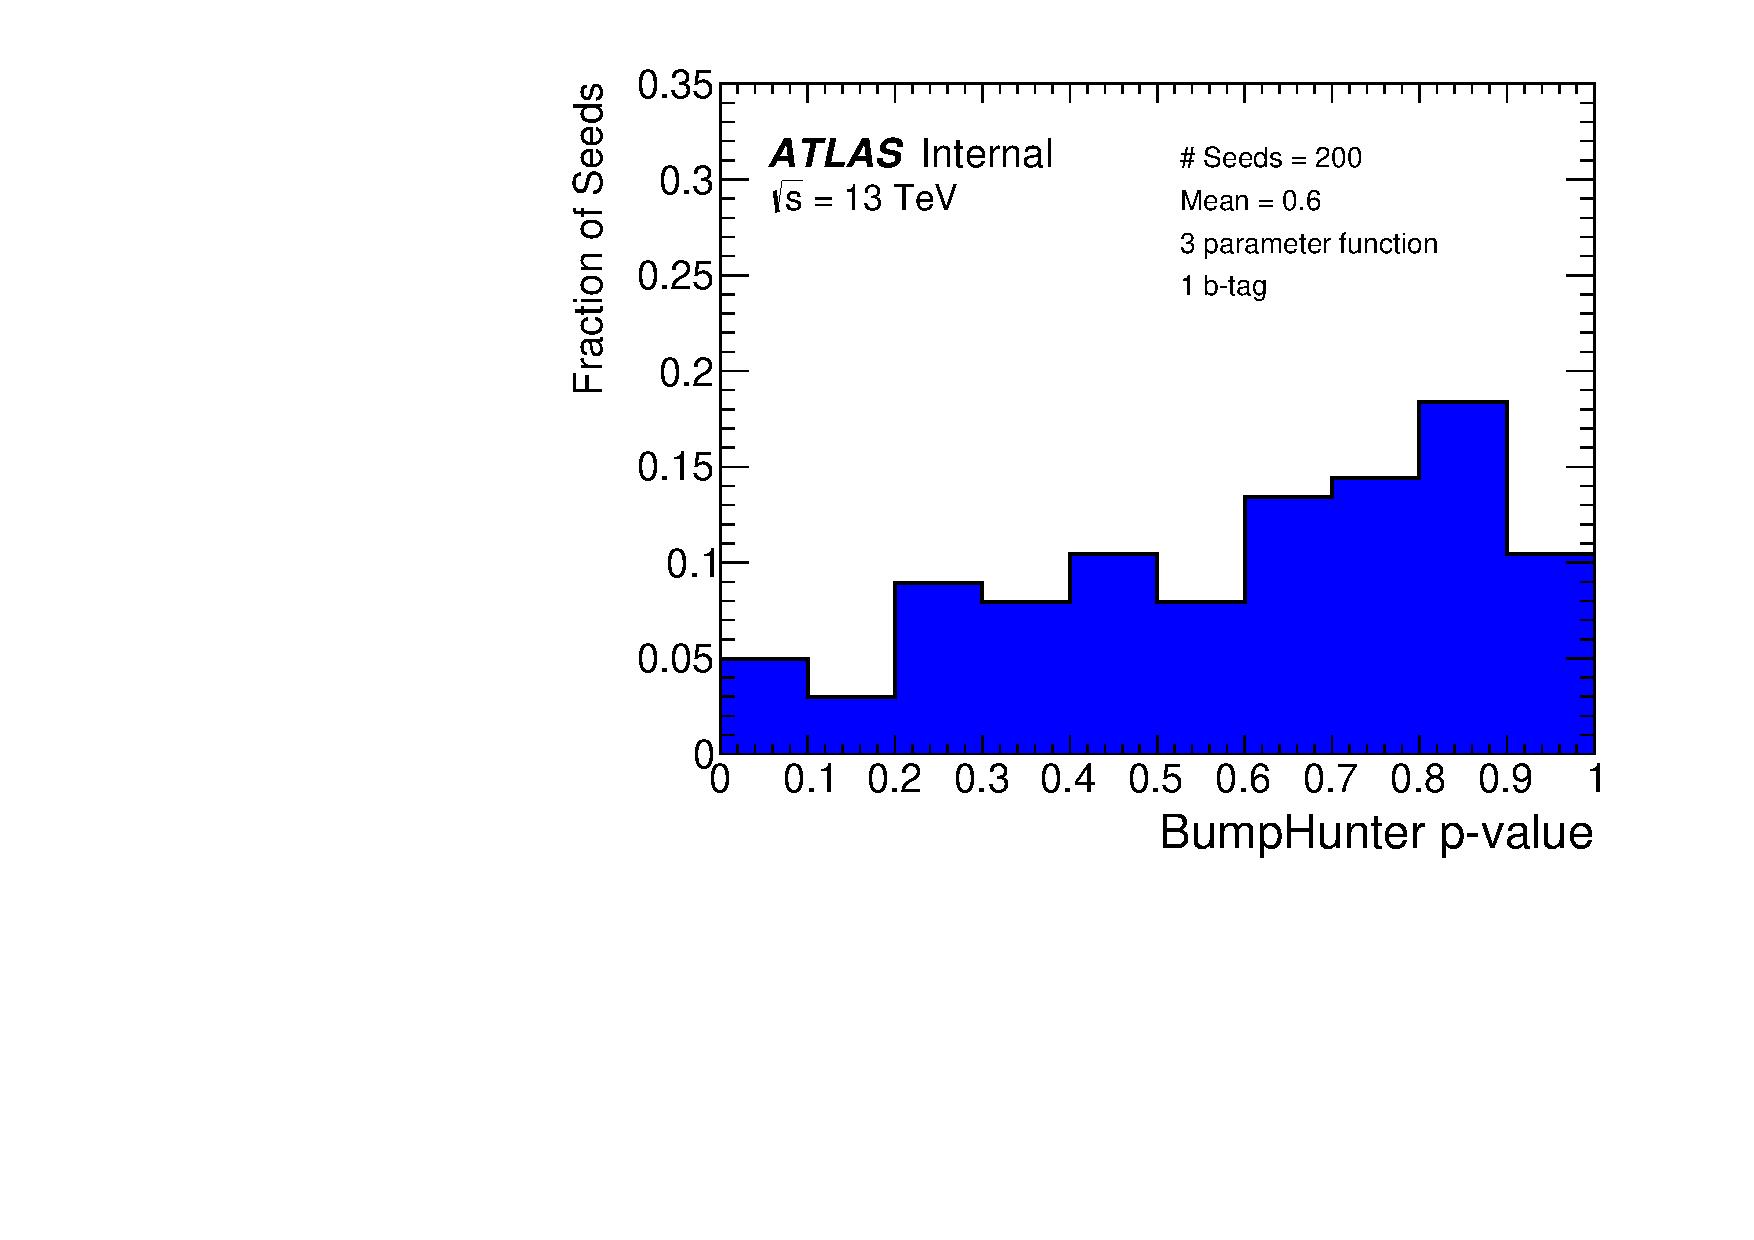
\includegraphics[width=0.32\linewidth, angle=0]{figs/Dibjet/ICHEP/SpuriousSignal/mbj_inc_fix_8585_pValHist_bumpHunter.pdf}}
  \subcaptionbox{DeficitHunter}{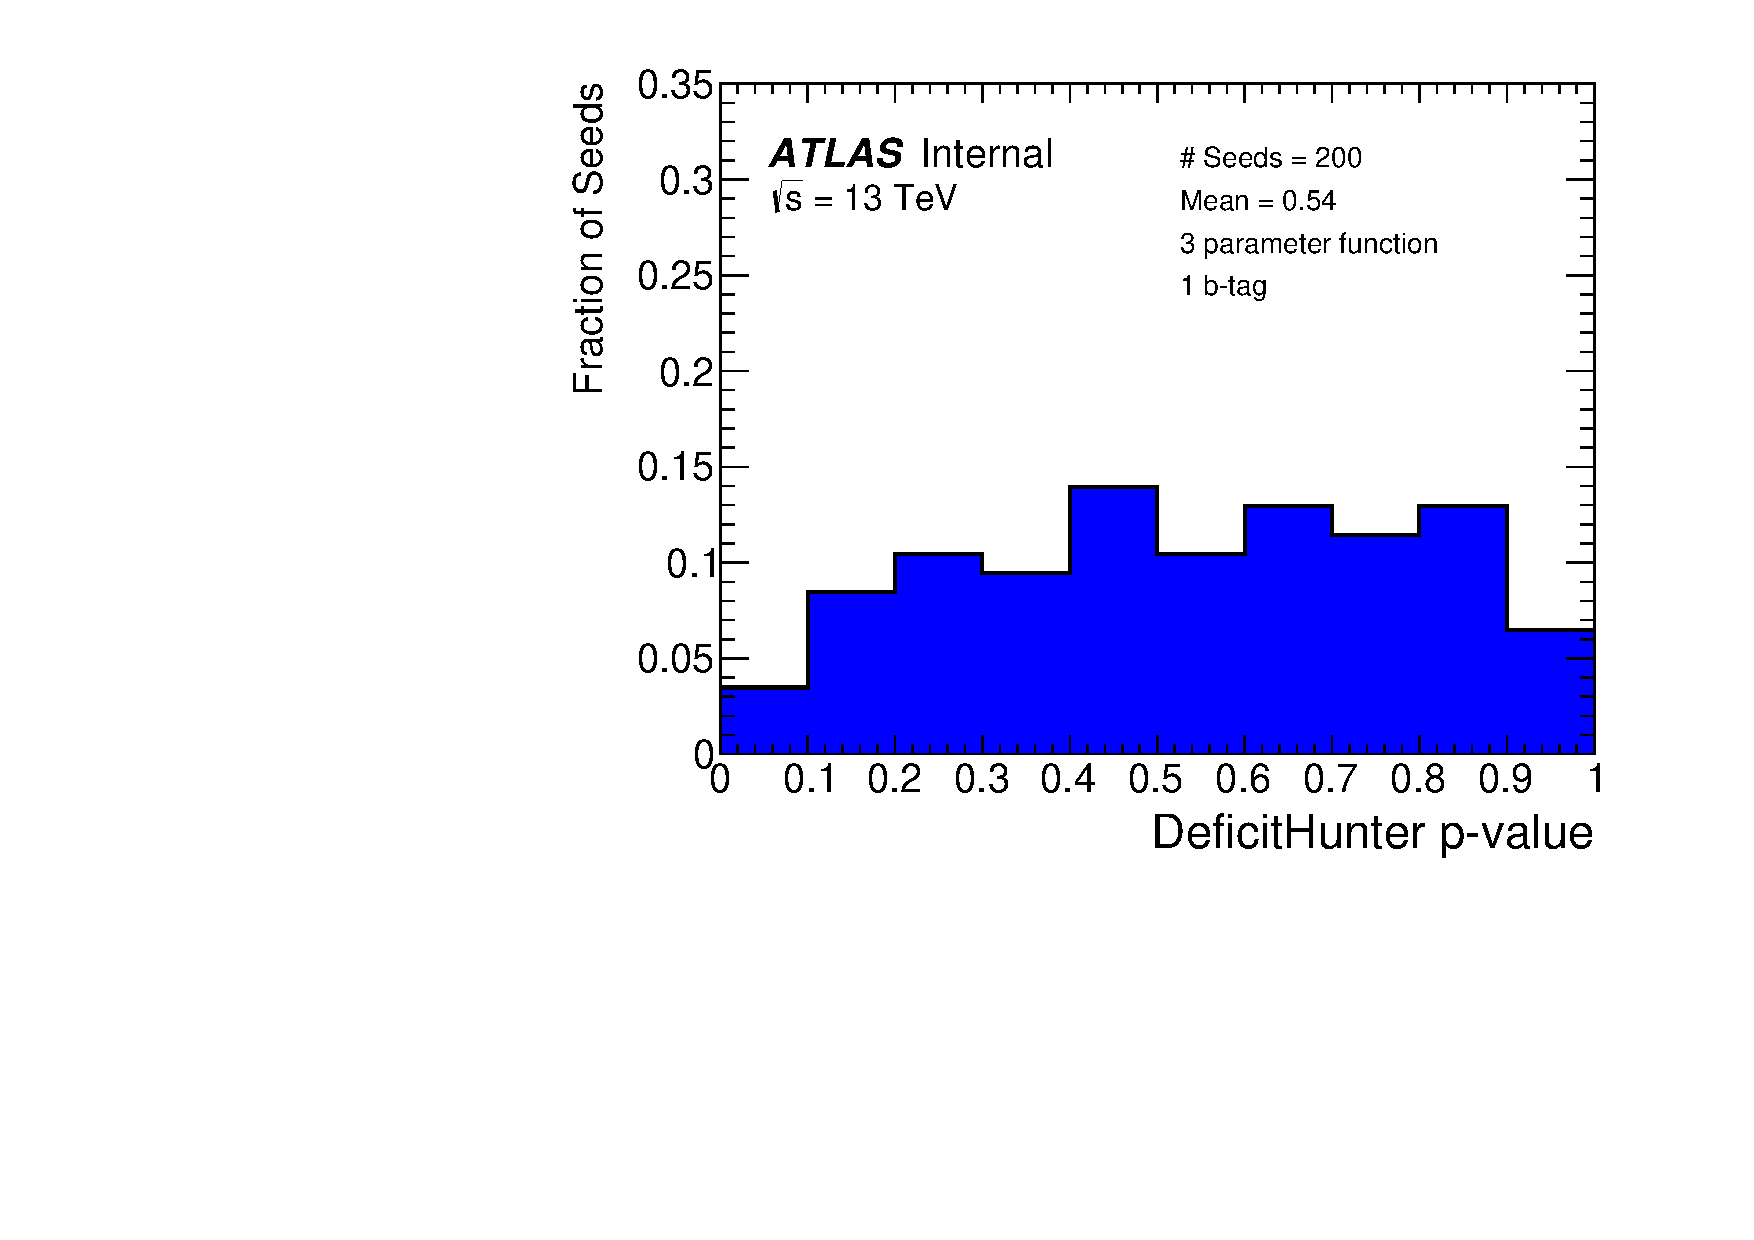
\includegraphics[width=0.32\linewidth, angle=0]{figs/Dibjet/ICHEP/SpuriousSignal/mbj_inc_fix_8585_pValHist_deficitHunter.pdf}}
  \subcaptionbox{$\chi^{2}$}{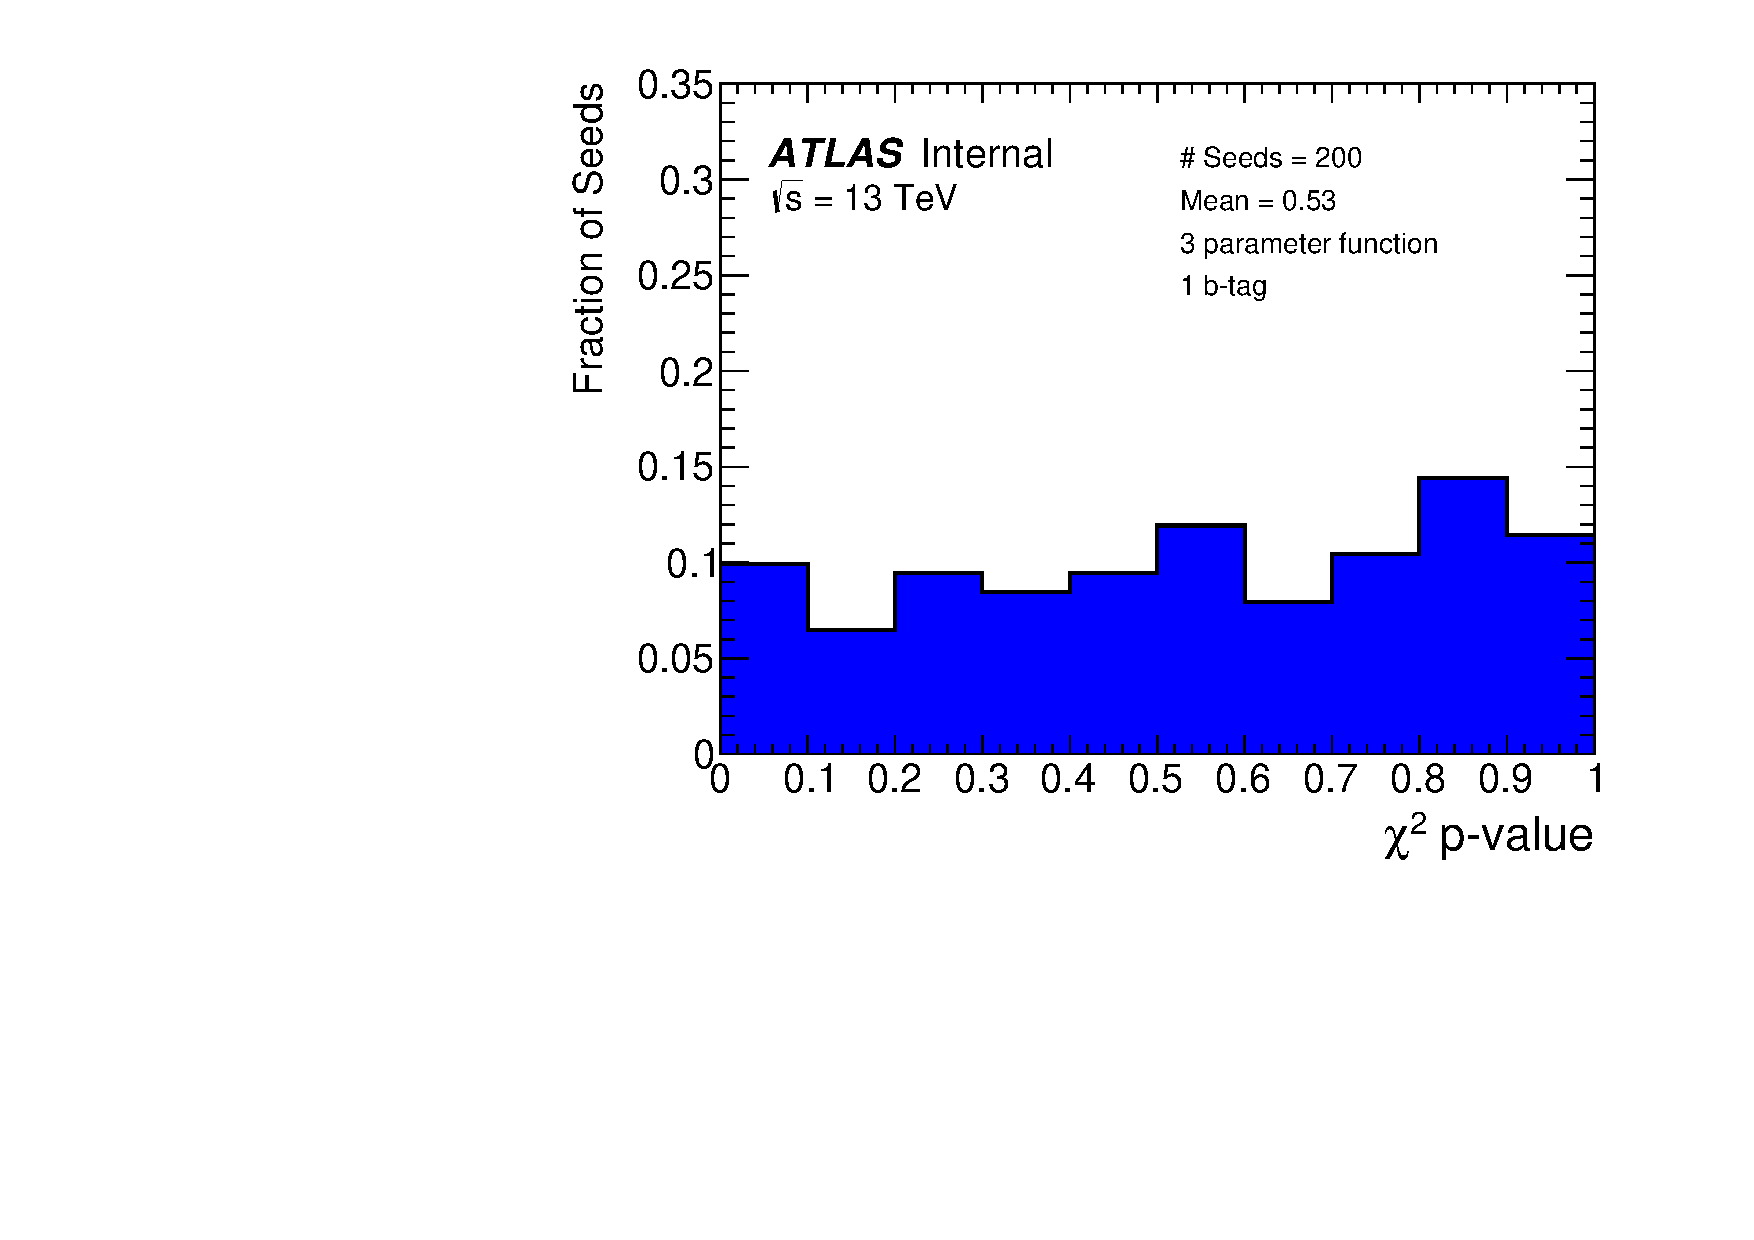
\includegraphics[width=0.32\linewidth, angle=0]{figs/Dibjet/ICHEP/SpuriousSignal/mbj_inc_fix_8585_pValHist_chi2.pdf}}
  \end{center}
  \caption{The distribution of (a) BumpHunter, (b) DeficitHunter and (c) $\chi^{2}$ $p$-values for fits to
    200 data-like invariant mass spectra in the $\geq1$ $b$-tag category.
    The \textit{Summer16+15} dataset event selection has been applied.}
  \label{fig:pValueHists_bj}
\end{figure}

\FloatBarrier

%\section{Flavour Fraction}
%\label{sec:FlavourFraction}
%
%\begin{figure}[!htb]
%  \begin{center}
%    \includegraphics[scale=0.8, angle=0]{figs/flavourFraction/backgroundFlavourComposition.pdf}
%  \end{center}
%  \caption{The dijet flavour composition of the simulated dijet background as a function of dijet mass, shown for the inclusive, ≥ 1 $b$-tag and 2 $b$-tag categories.}
%  \label{fig:flavourComposition}
%\end{figure}
  
\subsection{Search Phase}
\label{sec:bkg-summer_results}

It has been shown that the 3 parameter dijet fit function has a
sufficient number of parameters to provide an adequete background
description in both $b$-tagging categories in the fit region that has been chosen
and that there is no evidence that spurious signal can occur.
Hence, for the \verb|Summer16+15| data-set the 3 parameter fit function
provides a valid background estimation in both categories.

Figure~\ref{fig:bkg-summer_searchPhase} shows the final
\verb|Summer16+15| data-set fitted to with the 3 parameter fit function
in the 2 and $\geq1$ $b$-tag categories.
The upper panel shows the data compared to the background fit,
in addition the benchmark signal models with enhanced cross sections have been overlaid for each category.
The lower panel shows the significance of the difference between the data and background estimate.


\begin{figure}[!tb]
  \begin{center}
    \captionsetup[subfigure]{aboveskip=0pt,justification=centering}
   \subcaptionbox{2 $b$-tag}{\includegraphics[width=0.47\linewidth, angle=0]{figs/Dibjet/ICHEP/bkg-SearchPhase_bb.pdf}}
   \subcaptionbox{$\geq$1 $b$-tag}{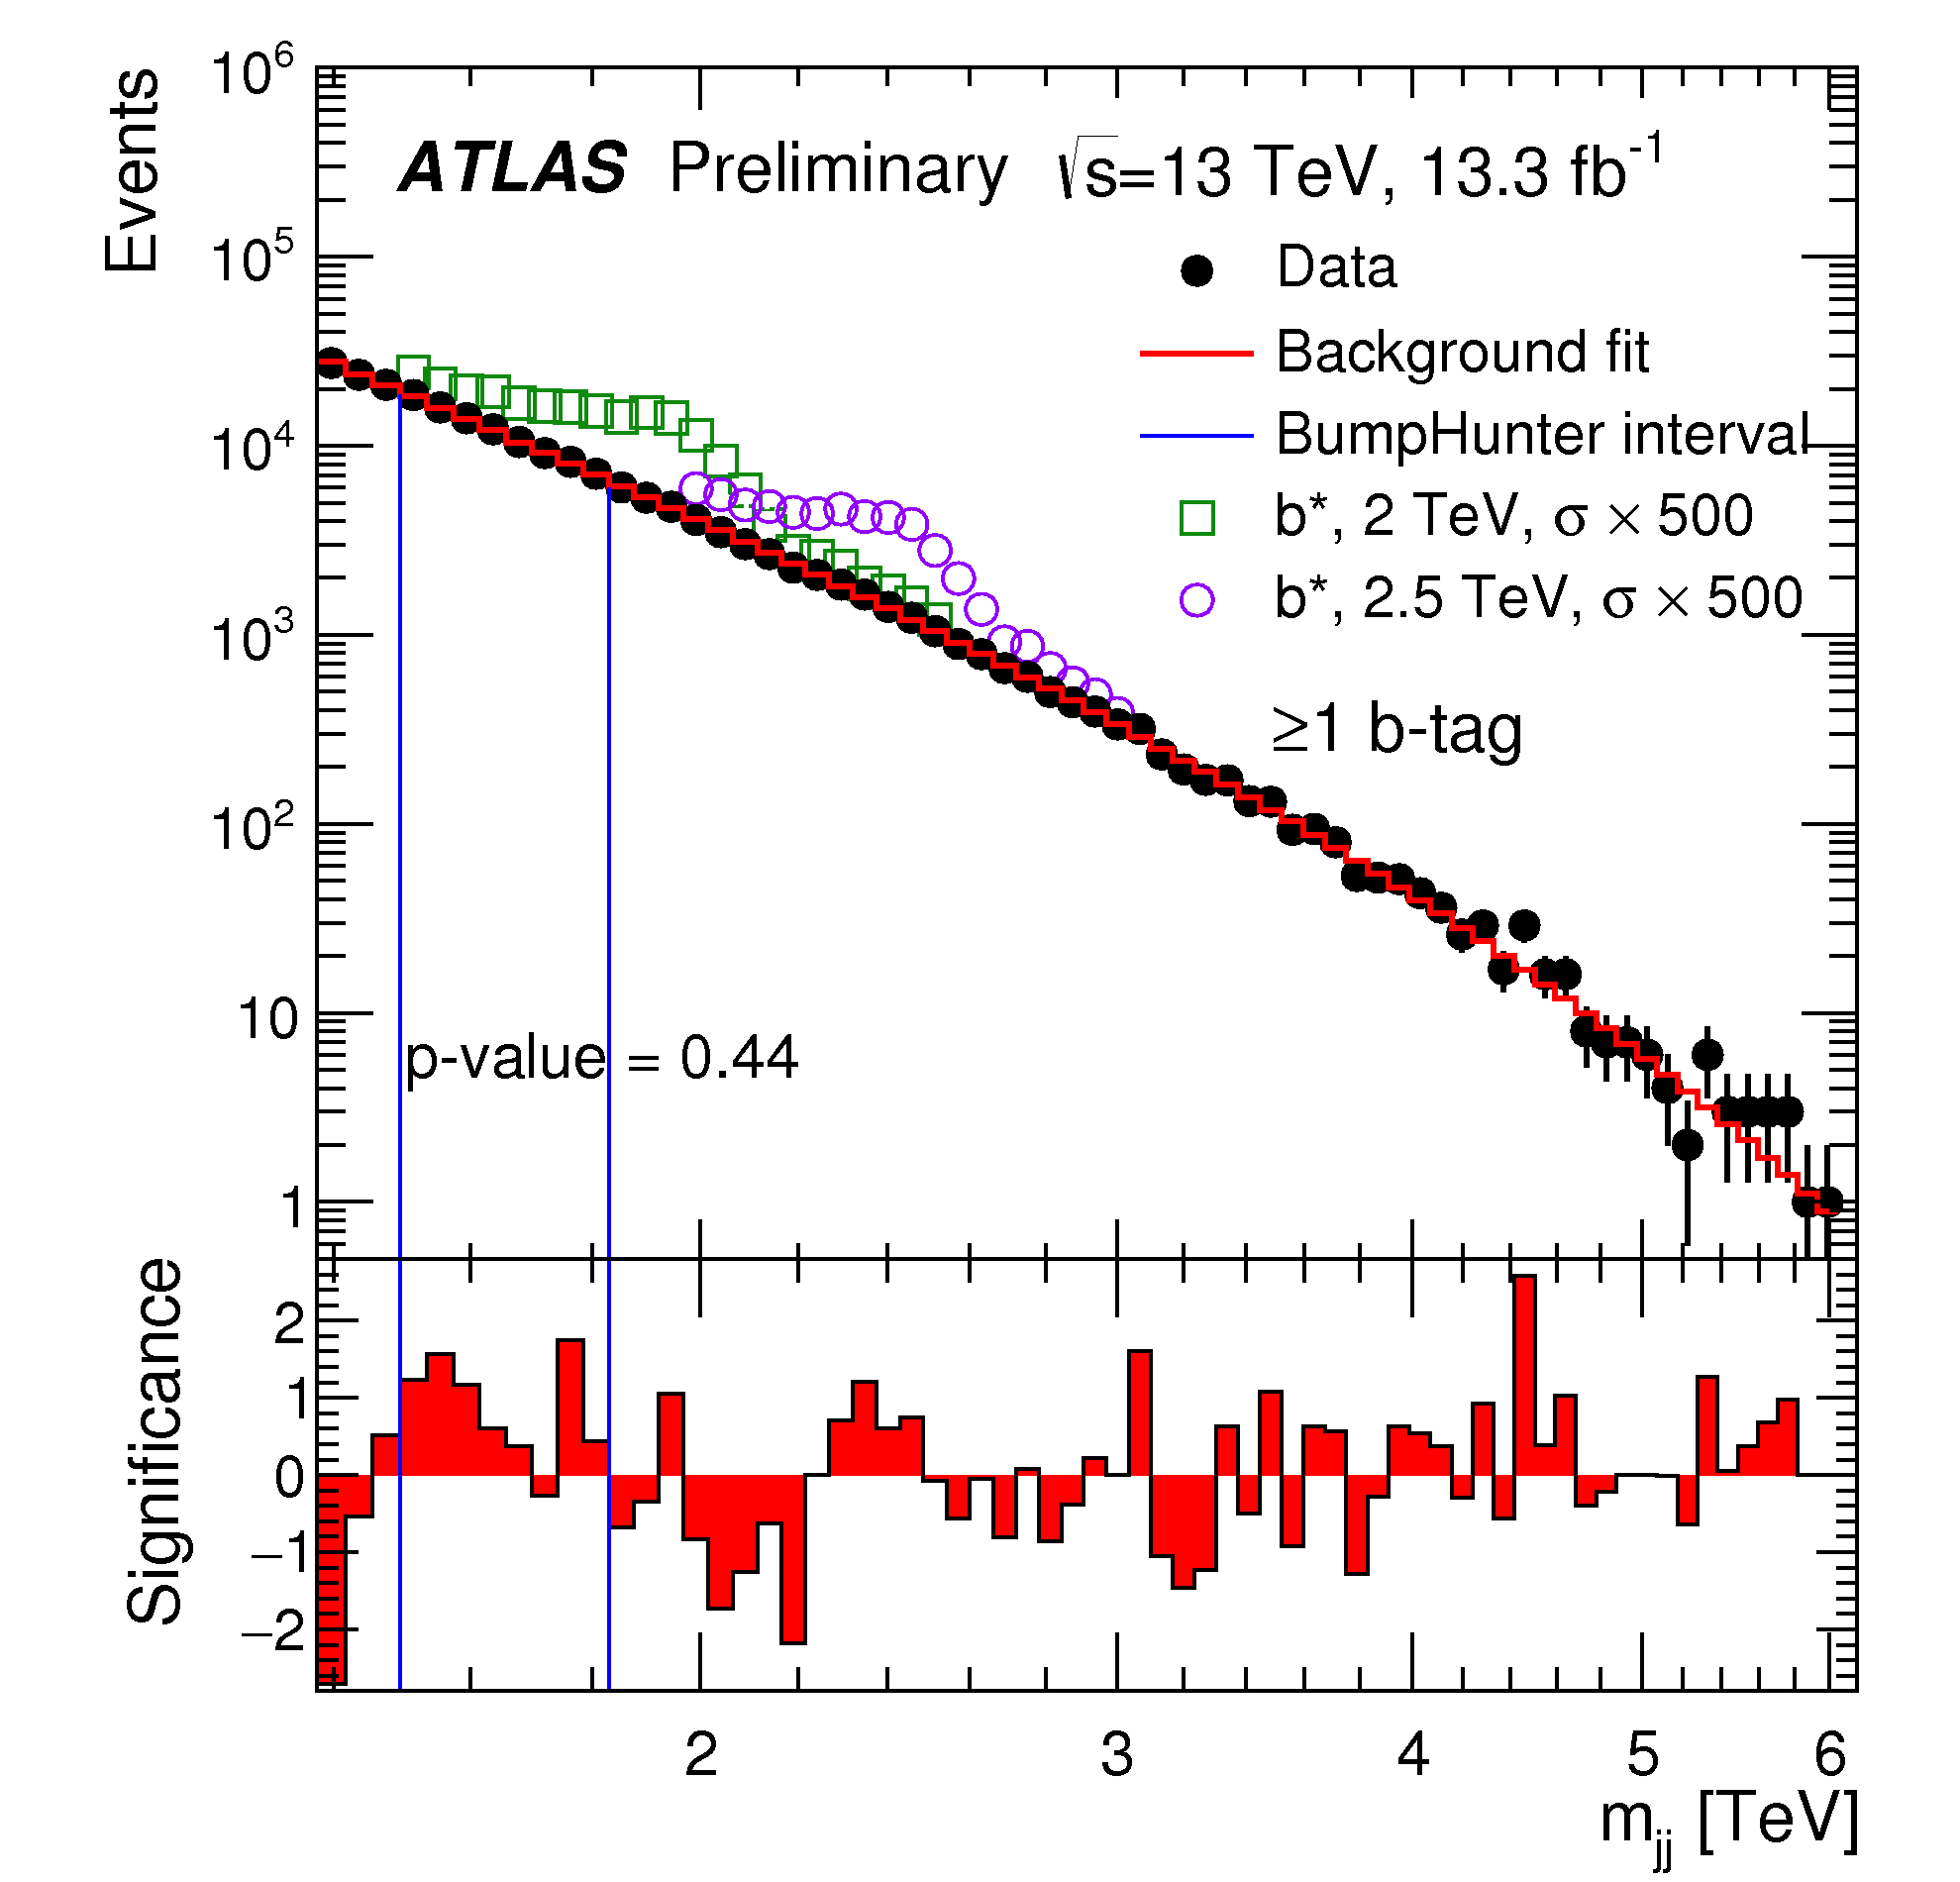
\includegraphics[width=0.47\linewidth, angle=0]{figs/Dibjet/ICHEP/bkg-SearchPhase_b.pdf}}
  \end{center}
  \caption[The final \textit{Summer16+15} data-set in the (a) 2 $b$-tag and the (b) $\geq$1 $b$-tag category,
            where the background has been modelled using the 3 parameter dijet fit function.
            The upper panel shows the data compared to the background estimate,
            benchmark signal models with enhanced cross sections are overlaid.
            The lower panel shows the significance of the difference between the data and the background estimate.
            The most discrepant excess as found by the BumpHunter algorithm is indicated by the vertical blue lines and the $p$-value of this excess is printed on the plot.]
          {The final \textit{Summer16+15} data-set in the (a) 2 $b$-tag and the (b) $\geq$1 $b$-tag category,
            where the background has been modelled using the 3 parameter dijet fit function.
            The upper panel shows the data compared to the background estimate,
            benchmark signal models with enhanced cross sections are overlaid.
            The lower panel shows the significance of the difference between the data and the background estimate.
            The most discrepant excess as found by the BumpHunter algorithm is indicated by the vertical blue lines and the $p$-value of this excess is printed on the plot
            ~\cite{dibjet-ichep_conf}.
          }
  \label{fig:bkg-summer_searchPhase}
\end{figure}

In both cases the BumpHunter algorithm has identified the most discrepant excess indicated
in the figure using vertical blue lines.
The BumpHunter $p$-value has been calculated using 10,000 pseudo-experiments.
The BumpHunter $p$-value is 0.60 in the 2 $b$-tag category
and 0.44 in the $\geq1$ $b$-tag category.
Hence, the conclusion of the search phase in the \verb|Summer16+15| data-set analysis
is that there is no signifcant excess found in either $b$-tag category.


\section{Full\_2016 Search Phase}
\label{sec:bkg-full}

SWiFt and ect...
